%*****************************************
\chapter{Theoretical Background}\label{ch:theoretical_background}
%*****************************************

Conceived in general terms, a filter is a device for removing unwanted components of a mixture. In accordance with this definition, in the technical sphere, a \emph{filter} refers to a system designed to extract information about a quantity of interest, using noisy observations of a process. That is, a filter delivers an estimate of the variables of principal interest, which is why it is also called an \emph{estimator}.

In the next section, we will present the filtering problem in a formal manner, followed by a comprehensive introduction of a generic framework to cope with it, the Bayesian filter. The Kalman filter presented in Section \ref{sec:Kalman} is suitable for linear models and additive white Gaussian noise. We deliberately chose to start from this special-case scenario, generalising step by step, as the Kalman filter is an easy to comprehend, straight forward solution to the filtering problem and its mechanism and underlying terminology is essential for the remainder of this thesis. In Section \ref{sec:extended_kalman}, we will introduce the extended Kalman filter, which uses linearisation around the latest state estimate in order to cope with non-linear models. A higher-order approximation of non-linear models is obtained by the unscented Kalman filter described in Section \ref{sec:unscented_kalman}. After elaborating on sequential Monte Carlo simulation, including sequential importance sampling in Section \ref{sec:importance_sampling} and resampling in Section \ref{sec:importance_resampling}, we focus on the importance of the proposal distribution in Section \ref{sec:importance_proposal}. In order to drop the Gaussian assumption and allow for arbitrary, multi-modal distributions, we introduce the generic particle filter in Section \ref{sec:particle}, followed by two concrete implementations, namely the bootstrap filter in Section \ref{sec:bootstrap_filter} and the unscented particle filter in Section \ref{sec:unscented_particle}. Finally, we will close this chapter with basic concepts of interval analysis in Section \ref{sec: interval_basic_concepts} including the notion of constraint satisfaction problems and set inversion problems in Sections \ref{sec:csp} and \ref{sec:sip}, respectively. Both types of problems will be encountered in the following Chapter \ref{ch:implementation} and will be tackled with either the \texttt{HC4} contractor described in Section \ref{sec:contractors} or the Set Inverter via Interval Analysis presented in Section \ref{sec:sivia}.



\section{The Filtering Problem}

Consider, as an example involving filter theory, the discrete-time dynamical system depicted in Figure \ref{fig:state_estimation}. The desired state vector of the system, $\bm{x}_k$, at the discrete time step $k$, is usually hidden and can only be observed by indirect measurements $\bm{z}_k$ that are a function of $\bm{x}_k$ and subject to noise. Equally, the equation describing the evolution of the state $\bm{x}_k$ is usually subject to errors, caused by effects not accounted for in the model. The dynamical system may be an underwater robot, in which case the elements of the state vector are constituted by its position and velocity, while the measuring system may be an inertial measurement unit producing the observation vector $\bm{z}_k$. The requirement of the filter is to deliver a reliable estimate $\hat{\bm{x}}_k$ of the actual state, by taking the measurement as well as prior information into account.

\tikzstyle{block} = [draw, rectangle, minimum height=3em, minimum width=6em]
\tikzstyle{output} = [coordinate]
\tikzstyle{pinstyle} = [pin edge={to-, thick, black}, align=center]

\begin{figure}[]
\centering
\resizebox{\textwidth}{!}{
\begin{tikzpicture}[auto, thick, rounded corners=1pt, node distance=3cm,>=latex']
    \node [block, align=center, 
    	pin={[pinstyle]below:System \\ errors}]
    	(dynamical) {Dynamical \\ system};
    \node [block, align=center, right of=dynamical, pin={[pinstyle]below:Measurement \\ errors}, node distance=4.5cm] (measuring) {Measuring \\ system};
    \node [block, align=center, right of=measuring, pin={[pinstyle]below:Prior \\ information}, node distance=4.5cm] (estimator) {Estimator};
    \node [output, right of=estimator] (output) {};
    
    \draw [->, align=center] (dynamical) -- node[name=x] {State \\ $\bm{x}_k$} (measuring);
    \draw [->, align=center] (measuring) -- node[name=y] {Observation \\ $\bm{z}_k$} (estimator);
    \draw [->, align=center] (estimator) -- node[name=y] {State \\ estimate \\ $\hat{\bm{x}}_k$} (output);
\end{tikzpicture}
}
\caption[Block diagram depicting the components involved in state estimation of a discrete-time dynamical system.]{Block diagram depicting the components involved in state estimation of a discrete-time dynamical system \cite{haykin2013adaptive}.} \label{fig:state_estimation}
\end{figure}

Assuming a stationary stochastic process with known statistical parameters as the mean and correlation function of the useful signal and the unwanted additive noise, the solution to the filtering problem is commonly known as the \emph{Wiener filter}. Yet, since the Wiener filter requires a priori information about the statistics of the data to be processed, it may not be optimal for non-stationary processes. For such an environment, in which the statistics are time-varying, it needs a filter that constantly adapts its parameters to optimise its output. A so-called \emph{adaptive filter} is a self-designing system that relies, in contrast to the non-recursive Wiener filter, on a recursive algorithm, allowing the filter to perform satisfactorily, even if there is no complete knowledge of the relevant signal characteristics. Provided the variations in the  statistics of the input data are sufficiently slow, the algorithm can track time variations and is thus suitable for non-stationary environments. In a stationary environment it converges to the optimum Wiener solution in some statistical sense after successive iterations.


\subsubsection{Generic State-space Model}

Now, let us consider the generic stochastic filtering problem in a dynamic state-space form:

\begin{equation}\label{eq:generic-state_dynamics}
  \bm{x}_k = \bm{\phi}_{k-1}(\bm{x}_{k-1}, \bm{u}_{k-1}, \bm{w}_{k-1}), \quad k > 0\,.
\end{equation}

\noindent
Here, $\bm{x}_k \in \mathbb{R}^{n_{\bm{x}}}$ is the state vector to be estimated, $k$ denotes the time step, and $\bm{\phi}_{k-1}: \mathbb{R}^{n_{\bm{x}}} \times \mathbb{R}^{n_{\bm{u}}} \times \mathbb{R}^{n_{\bm{w}}} \rightarrow \mathbb{R}^{n_{\bm{x}}}$ is the known, possibly non-linear state transition function at time $k-1$. The control vector $\bm{u}_{k-1} \in \mathbb{R}^{n_{\bm{u}}}$ represents an exogenous input to the system and $\bm{w}_{k-1} \in \mathbb{R}^{n_{\bm{w}}}$ represents a white noise sequence, usually referred to as the process noise. The state vector is related to the observation or measurement of the process, $\bm{z}_k \in \mathbb{R}^{n_{\bm{z}}}$, by

\begin{equation}\label{eq:generic-measurement}
  \bm{z}_k = \bm{h}_{k}(\bm{x}_{k}, \bm{v}_{k}), \quad k > 0\,,
\end{equation}

\noindent
where $\bm{h}_k: \mathbb{R}^{n_{\bm{x}}} \times \mathbb{R}^{n_{\bm{v}}} \rightarrow \mathbb{R}^{n_{\bm{z}}}$ is a known, possibly non-linear transformation from state variables to measurement variables and $\bm{v}_{k} \in \mathbb{R}^{n_{\bm{v}}}$ represents a white noise sequence, usually referred to as the measurement noise. Note that here we do not assume additivity of the noise sources. A block diagram of the non-linear discrete-time dynamic system and its observation is depicted in Figure \ref{fig:non-linear-dynamic-system}, where $z^{-1}$ denotes the unit-delay and $\bm{I}_{n_{\bm{x}}}$ the $n_{\bm{x}}\times n_{\bm{x}}$ identity matrix.
%In the following section we will present a framework that utilises the measurements as well as available prior information to tackle the filtering problem.

\tikzstyle{block} = [draw, rectangle, minimum height=0.8cm, minimum width=0.8cm]
\tikzstyle{sum} = [draw, circle]
\tikzstyle{output} = [coordinate]
\tikzstyle{input} = [coordinate]

\begin{figure}[t]
\centering
\begin{tikzpicture}[auto, thick, node distance=1.5cm,>=latex']
	
	\node [block] (phi) {$\bm{\phi}_{k-1}$};
	\node [input, above of=phi] (w) {};
    \node [block, align=center, 
    	right of=phi, node distance=3cm] (H) {$\bm{h}_k$};
    \node [input, left of=phi, node distance=2cm] (u) {};
    \node [input, above of=H] (v) {};
    \node [output, right of=H, node distance=1.5cm] (out) {};
    
    \draw [->] (phi) -- node[] {$\bm{x}_k$} node[name=x_k, pos=0.5] {} (H);
    \node [block, below of=phi, node distance=1.8cm] (delay) {$z^{-1_{ }}\bm{I}_{n_{\bm{z}}}$};
    \draw [->] (delay) -- node [] {$\bm{x}_{k-1}$} (phi);
    \draw [->] (w) -- node [label={left:$\bm{w}_{k-1}$}, pos=0.29]{} (phi);
    \draw [->] (u) -- node[] {$\bm{u}_{k-1}$} (phi);
    \draw [->] (v) -- node [label={left:$\bm{v}_{k}$}, pos=0.29]{}  (H);
    \draw [->] (x_k) |- (delay);
    \draw [->] (H) -- node[pos=0.77, name=xk_hat] {$\bm{z}_k$} (out);
         
\end{tikzpicture}


\caption[Block diagram depicting a non-linear discrete-time dynamical system, its internal state, and its observation.]{Block diagram depicting a non-linear discrete-time dynamical system, its internal state $\bm{x}_{k}$, and its observation $\bm{z}_{k}$.} \label{fig:non-linear-dynamic-system}
\end{figure}

\section{Recursive Bayesian Estimation}\label{sec:bayesian_estimation}

Provided the system dynamics model and the measurement model can be expressed in a probabilistic form, a Bayesian approach to solving the filtering problem may be adopted. The formal \emph{Bayesian filter} constitutes a general unifying framework for sequential state estimation, at least in a conceptual sense \cite{haykin2009neural}. We will only go into detail as far as necessary for the treatment of the subject matter of this thesis. A complete mathematical derivation of the Bayesian filter can be found in \cite{thrun2005probabilistic}.


The system model given by Equation \ref{eq:generic-state_dynamics} implicitly assumes that the state $\bm{x}_k$ depends only on the immediate past state $\bm{x}_{k-1}$ and the control input $\bm{u}_{k-1}$. Thus, it defines a first-order discrete Markov process and has an equivalent probabilistic description given by the conditional probability distribution $p(\bm{x}_k\,|\,\bm{x}_{k-1}, \bm{u}_{k-1})$, with the initial state distributed according to 

\begin{equation}\label{eq:initial_markov}
  p(\bm{x}_0\,|\,\bm{z}_0) = p(\bm{x}_0)\,,
\end{equation}

\noindent
where $\bm{z}_0$ denotes the empty measurement.

Likewise, the measurement model given by Equation \ref{eq:generic-measurement} has an equivalent probabilistic description given by the conditional probability density $p(\bm{z}_k\,|\,\bm{x}_{k})$. Here, we implicitly assume that if we knew the state $\bm{x}_{k}$ and were to predict the measurement $\bm{y}_{k}$, no past measurement or control input would provide us additional information. This conditional independence given the state, the Markov property, and the fact that we cannot observe the state directly let us describe our system using the hidden Markov model depicted in Figure \ref{fig:generic-ss-model}. In the remainder of this chapter, we will use the notation below:

% depicted in Table \ref{tab:notation_bayes}.

\begin{table*}[h]
\begin{tabularx}{\textwidth}{lX}
$\bm{X}_k$          		 & \emph{sequence of states}, denoting $\{\bm{x}_i\}^k_{i = 0}$. \\
$\bm{U}_k$          		 & \emph{sequence of control inputs}, denoting $\{\bm{u}_i\}^k_{i = 0}$. \\
$\bm{Z}_k$          		 & \emph{sequence of observations}, denoting $\{\bm{z}_i\}^k_{i = 1}$. \\
$p(\bm{x}_k\,|\,\bm{Z}_{k-1}, \bm{U}_{k-1})$ & \emph{predictive distribution} of the state $\bm{x}_k$ at the current time $k$, given the entire sequence of observations and the entire sequence of control inputs up to and including time $k-1$. \\
$p(\bm{x}_k\,|\,\bm{Z}_{k}, \bm{U}_{k-1})$ & \emph{posterior distribution} of the current state $\bm{x}_k$, given the entire sequence of observations up to and including the current time $k$ and the entire sequence of control inputs up to and including time $k-1$; this distribution is commonly referred to as simply the posterior. \\
$p(\bm{x}_k\,|\,\bm{x}_{k-1}, \bm{u}_{k-1})$ & \emph{state-transition distribution} of the current state $\bm{x}_k$, given the immediate past state $\bm{x}_{k-1}$ and control input $\bm{u}_{k-1}$; this distribution is defined in terms of the system model and is commonly referred to as the transition prior or simply the prior. \\
$p(\bm{z}_k\,|\,\bm{x}_{k})$ & \emph{likelihood function} of the current observation $\bm{z}_k$, given the current state $\bm{x}_{k}$. This function is defined in terms of the observation model.
\end{tabularx}
%\caption{Conditional probability distributions used in recursive Bayesian state estimation.}
%\label{tab:notation_bayes}
\end{table*}

\tikzstyle{state}=[shape=circle,draw=black!100,fill=black!10, minimum width=1.2cm]
\tikzstyle{input}=[shape=circle,draw=black!100,fill=white!100,  minimum width=1.2cm]
\tikzstyle{observation}=[shape=rectangle,draw=black!100,fill=white!100, minimum width=1.2cm]
\tikzstyle{lightedge}=[<-,dotted]
\tikzstyle{mainstate}=[state,thick]
\tikzstyle{mainedge}=[<-,thick]


\begin{figure}[t]
\begin{center}
\begin{tikzpicture}[]
% 1st column
\node[left] at (-1.2,5) {Input};
\node[left] at (-1.2,3) {State};
\node[left] at (-1.2,1) {Observation};
% 2st column
\node[input] (u_k-1) at (0,5) {$\bm{u}_{k-1}$};
\node[state] (x_k-1) at (0,3) {$\bm{x}_{k-1}$};
\node[observation] (y_k-1) at (0,1) {$\bm{z}_{k-1}$}
	edge[mainedge] node[auto,swap] {$\bm{h}_{k-1}$} (x_k-1);
\node at (1,3.6) {$\bm{\phi}_{k-1}$};
% 3rd column
\node[input] (u_k) at (2,5) {$\bm{u}_{k}$}
    edge[lightedge] (u_k-1);
\node[state] (x_k) at (2,3) {$\bm{x}_{k}$}
    edge[mainedge] (x_k-1)
    edge [<-,bend right=35, thick] (u_k-1);
\node[observation] (y_k) at (2,1) {$\bm{z}_{k}$}
	edge[mainedge] node[auto,swap] {$\bm{h}_{k}$} (x_k);
\node at (3,3.6) {$\bm{\phi}_{k}$};
% 4th column
\node[input] (u_k+1) at (4,5) {$\bm{u}_{k+1}$}
    edge[lightedge] (u_k);
\node[state] (x_k+1) at (4,3) {$\bm{x}_{k+1}$}
    edge[mainedge] (x_k)
    edge [<-,bend right=35, thick] (u_k);
\node[observation] (y_k+1) at (4,1) {$\bm{z}_{k+1}$}
	edge[mainedge] node[auto,swap] {$\bm{h}_{k+1}$} (x_k+1);
\end{tikzpicture}
\end{center}
\caption[Hidden Markov model of a non-linear discrete-time dynamical system.]{Hidden Markov model of a non-linear discrete-time dynamical system, characterising the evolution of the control inputs, states, and observations.}
\label{fig:generic-ss-model}
\end{figure}


Now, the aim of the Bayesian filter is to determine the posterior distribution $p(\bm{x}_k\,|\,\bm{Z}_{k}, \bm{U}_{k-1})$, which embodies the entire knowledge that we have about the state $\bm{x}_k$ at time $k$, after being given all the control inputs $\bm{U}_{k-1}$ and having received the entire observation sequence $\bm{Z}_k$. Given this probability distribution, we can determine an optimal estimator under a specified performance criterion, as for instance the minimum mean-squared error estimator. Then, the optimal state estimate $\hat{\bm{x}}_k$ is determined by the mean of the posterior probability distribution, 

\begin{equation}
  \hat{\bm{x}}_k = \mathbb{E}\big[\bm{x}_k\,|\,\bm{Z}_{k}, \bm{U}_{k-1}\big] = \int \bm{x}_k p(\bm{x}_k\,|\,\bm{Z}_{k}, \bm{U}_{k-1}) d\bm{x}_k\,.
\end{equation}

\noindent
In order to assess the confidence in the estimated state, we compute the covariance matrix as

\begin{equation}
\begin{split}
  \bm{P}_k &= \mathbb{E}\Big[(\bm{x}_k - \hat{\bm{x}}_{k})(\bm{x}_k - \hat{\bm{x}}_{k})^T\Big] \\
  &= \int (\bm{x}_k - \hat{\bm{x}}_{k})(\bm{x}_k - \hat{\bm{x}}_{k})^T p(\bm{x}_k\,|\,\bm{Z}_{k}, \bm{U}_{k-1}) d\bm{x}_k\,.
\end{split}
\end{equation}


 The posterior distribution can be constructed recursively in two steps, namely by a prediction and an update operation:

\begin{enumerate}
\item \emph{Time update}: given the observation sequence $\bm{Z}_{k-1}$ and the control sequence $\bm{U}_{k-2}$, the predictive distribution is computed according to the Chapman-Kolmogorov identity:

\begin{equation}\label{eq:chapman_kolmogorov}
\begin{split}
  \underbrace{p(\bm{x}_k\,|\,\bm{Z}_{k-1}, \bm{U}_{k-1})}_{\substack{\text{Predictive} \\ \text{distribution}}}
  &= \int p(\bm{x}_k\,|\,\bm{x}_{k-1}, \bm{Z}_{k-1}, \bm{U}_{k-1}) \\
  &\mathrel{\phantom{iiiiiiii}} \cdot\:p(\bm{x}_{k-1}\,|\,\bm{Z}_{k-1}, \bm{U}_{k-1}) d\bm{x}_{k-1} \\
  &= \int \underbrace{p(\bm{x}_k\,|\,\bm{x}_{k-1}, \bm{u}_{k-1})}_\text{Prior} \\
  &\mathrel{\phantom{iiiiiiii}} \cdot \underbrace{p(\bm{x}_{k-1}\,|\,\bm{Z}_{k-1}, \bm{U}_{k-2})}_\text{Old posterior} d\bm{x}_{k-1}\,.
  \end{split}
\end{equation}

\noindent
Here, we used the Markov property:

\begin{equation}\label{eq:markov_property}
  p(\bm{x}_k\,|\,\bm{x}_{k-1}, \bm{Z}_{k-1}, \bm{U}_{k-1}) = p(\bm{x}_k\,|\,\bm{x}_{k-1}, \bm{u}_{k-1})\,,
\end{equation}

\noindent
and the fact that the old posterior is conditionally independent of future control inputs, so that the following holds:

\begin{equation}
  p(\bm{x}_{k-1}\,|\,\bm{Z}_{k-1}, \bm{U}_{k-1}) = p(\bm{x}_{k-1}\,|\,\bm{Z}_{k-1}, \bm{U}_{k-2})\,.
\end{equation}


\item \emph{Measurement update}: exploiting the current observation $\bm{z}_{k}$ and applying Bayes' theorem, we can compute the updated posterior as follows: 

\begin{equation}\label{eq:updated_posterior}
\begin{split}
  \underbrace{p(\bm{x}_k\,|\,\bm{Z}_{k}, \bm{U}_{k-1})}_{\substack{\text{Updated} \\ \text{posterior}}} &= p(\bm{x}_k\,|\,\bm{z}_{k}, \bm{Z}_{k-1}, \bm{U}_{k-1}) \\
  &= \frac{p(\bm{z}_k\,|\,\bm{x}_{k}, \bm{Z}_{k-1}, \bm{U}_{k-1}) p(\bm{x}_k\,|\,\bm{Z}_{k-1}, \bm{U}_{k-1})}{p(\bm{z}_{k}\,|\,\bm{Z}_{k-1}, \bm{U}_{k-1})} \\
  &= \underbrace{p(\bm{z}_k\,|\,\bm{x}_{k})}_{\substack{\text{Likelihood} \\ \text{function}}} \underbrace{p(\bm{x}_k\,|\,\bm{Z}_{k-1}, \bm{U}_{k-1})}_{\substack{\text{Predictive} \\ \text{distribution}}} \eta^{-1} \,,
\end{split}
\end{equation}

\noindent
where the normalising constant $\eta$ is given by

\begin{equation}\label{eq:partition_function}
\begin{split}
\eta &= p(\bm{z}_k\,|\,\bm{Z}_{k-1}, \bm{U}_{k-1}) \\ 
  &= \int p(\bm{z}_k\,|\,\bm{x}_{k}) p(\bm{x}_{k}\,|\,\bm{Z}_{k-1}, \bm{U}_{k-1}) d\bm{x}_{k}\,.
\end{split}
\end{equation}

\noindent
Note how in the last transformation step of Equation \ref{eq:updated_posterior} we used conditional independence given the state, that is
 
 \begin{equation}\label{eq:markov_property_observation}
  p(\bm{z}_k\,|\,\bm{x}_{k}, \bm{Z}_{k-1}, \bm{U}_{k-1}) = p(\bm{z}_k\,|\,\bm{x}_{k})\,.
\end{equation}
 
\end{enumerate}


The Bayesian filter is the optimal conceptual solution to the recursive estimation problem. However, due to the multi-dimensional integration, a closed-form algorithm can only be obtained in a few special cases. If the probability distributions $p(\bm{x}_0)$, $p(\bm{x}_k\,|\,\bm{x}_{k-1}, \bm{u}_{k-1})$, and $p(\bm{z}_k\,|\,\bm{x}_{k})$ are Gaussian and the dynamic system is described by a linear model, the posterior distribution remains Gaussian and the Equations \ref{eq:chapman_kolmogorov} and \ref{eq:updated_posterior} reduce to the celebrated Kalman filter, which is described in the following section. Figure \ref{fig:filter_overview} compares different Bayesian filters that are discussed in further detail below.



\begin{figure}[t]
\begin{center}
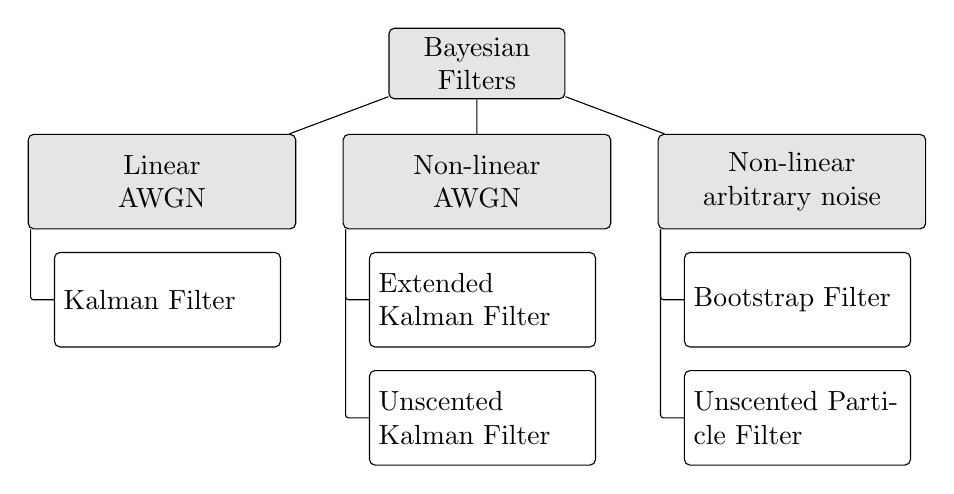
\begin{tikzpicture}[
	level 1/.style = {sibling distance=40mm, minimum height=1.2cm},
	  edge from parent/.style={-,draw},
	  >=latex,
  basic/.style   = {draw, text width=2cm, rounded corners=2pt, rectangle, thin, node distance=1.5cm},
  root/.style    = {basic, align=center, fill=black!10, text width=2cm},
  level 2/.style = {basic, align=center, fill=black!10, text width=9em},
  level 3/.style = {basic, align=left, text width=7.5em, minimum height=1.2cm}]
	
	% root of the the initial tree, level 1
	\node[root] {Bayesian Filters}
	% The first level, as children of the initial tree
	  child {node[level 2] (c1) {Linear \\ AWGN}}
	  child {node[level 2] (c2) {Non-linear \\ AWGN}}
	  child {node[level 2] (c3) {Non-linear \\ arbitrary noise}};
	
	% The second level, relatively positioned nodes
	\begin{scope}[every node/.style={level 3}]
	\node [below of = c1, xshift=2pt] (c11) {Kalman Filter};
	
	\node [below of = c2, xshift=2pt] (c21) {Extended \\ Kalman Filter};
	\node [below of = c21] (c22) {Unscented \\ Kalman Filter};
	
	\node [below of = c3, xshift=2pt] (c31) {Bootstrap Filter};
	\node [below of = c31] (c32) {Unscented Particle Filter};
	\end{scope}
	
	% lines from each level 1 node to every one of its "children"
	\foreach \value in {1}
	  \draw[-, rounded corners=1pt] (c1.200) |- (c1\value.west);
	
	\foreach \value in {1,...,2}
	  \draw[-, rounded corners=1pt] (c2.200) |- (c2\value.west);
	
	\foreach \value in {1,...,2}
	  \draw[-, rounded corners=1pt] (c3.200) |- (c3\value.west);
\end{tikzpicture}
\end{center}
\caption[Comparison of different Bayesian filters used in self-localisation of mobile robots.]{Comparison of different Bayesian filters used in self-localisation of mobile robots. AWGN denotes additive white Gaussian noise.}
\label{fig:filter_overview}
\end{figure}


\section{Kalman Filters}

The \emph{Kalman filter} provides an efficient means to analytically compute the evolving sequence of posterior distributions of a linear dynamic system that is perturbed by additive white Gaussian noise \cite{maybeck2002stochastic}. Named after Rudolf E. Kalman, who 1960 published his famous paper describing a recursive solution to the discrete-data linear filtering problem \cite{kalman_1960}, the Kalman filter has been the subject of extensive research, which is due, to a large extent, to the advances in digital computing \cite{welch2014}. The Kalman filter and its many variations find applications in radar tracking, navigation, and orientation estimation, among others. \citeauthor{zarchan2009fundamentals} stated in \cite{zarchan2009fundamentals}: ``With the possible exception of the fast Fourier transform, Kalman filtering is probably the most important algorithmic technique ever devised.'' We will now proceed to formally introduce the Kalman filter, followed by two of its variations for non-linear models in the subsequent sections.

\subsection{The Kalman Filter}\label{sec:Kalman}

Let $\bm{x}_k \in \mathbb{R}^{n_{\bm{x}}}$ be the state vector of a discrete-time controlled process, governed by the \emph{linear} stochastic difference equation 

\begin{equation}\label{eq:time_dynamical_system_plant}
  \bm{x}_k = \bm{\Phi}_{k-1}\bm{x}_{k-1}+\bm{B}_{k-1}\bm{u}_{k-1}+\bm{w}_{k-1}\,,
\end{equation}

\noindent
where the index $k$ again denotes discrete time. The $n_{\bm{x}} \times n_{\bm{x}}$ state transition matrix $\bm{\Phi}_{k-1}$ relates the state at the previous time step $k-1$ to the state at the current step $k$ and the $n_{\bm{x}} \times n_{\bm{u}}$ matrix $\bm{B}_{k-1}$ relates the known, optional control input $\bm{u}_{k-1} \in \mathbb{R}^{n_{\bm{u}}}$ to the state $\bm{x}_k$. Let $\bm{z}_k \in \mathbb{R}^{n_{\bm{z}}}$ denote the measurement vector of this process, which is related to the state by the linear measurement model

\begin{equation}\label{eq:time_dynamical_system_measurement}
  \bm{z}_k = \bm{H}_{k}\bm{x}_{k}+\bm{v}_{k}\,,
\end{equation}

\noindent
 where the $n_{\bm{z}} \times n_{\bm{x}}$ measurement matrix $\bm{H}_{k}$ relates the state $\bm{x}_k$ to the measurement $\bm{z}_k$. The $n_{\bm{x}}\times1$ vector $\bm{w}_k$ and the $n_{\bm{z}}\times1$ vector $\bm{v}_k$ in Equation \ref{eq:time_dynamical_system_plant} and \ref{eq:time_dynamical_system_measurement} represent the additive process and measurement noise, respectively, modelled as zero-mean, Gaussian white noise,

\begin{equation}\label{eq:process_noise}
  \bm{w}_{k} \sim \mathcal{N}(0,\bm{Q}_k)\,,
\end{equation}

\begin{equation}\label{eq:measurement_noise}
  \bm{v}_{k} \sim \mathcal{N}(0,\bm{R}_k)\,,
\end{equation}
 
\noindent
with the \emph{process noise covariance matrix} $\bm{Q}_k$ and the \emph{measurement noise covariance matrix} $\bm{R}_k$.

\tikzstyle{block} = [draw, rectangle, minimum height=0.8cm, minimum width=0.8cm]
\tikzstyle{sum} = [draw, circle]
\tikzstyle{output} = [coordinate]
\tikzstyle{input} = [coordinate]

\begin{figure}
\centering
\resizebox{\textwidth}{!}{
\begin{tikzpicture}[auto, thick, node distance=1.5cm,>=latex']
	
	\node [sum] (sum1) {$\sum$};
	\node [block, align=center, left of=sum1, node distance=1.5cm] (b) {$\bm{B}_{k-1}$};
	\node [input, above of=sum1] (w) {};
    \node [block, align=center, 
    	right of=sum1, node distance=3cm] (H) {$\bm{H}_k$};
    \node [block, align=center, below of=sum1, node distance=1.8cm] (phi) {$\bm{\Phi}_{k-1}$};
    \node [input, above of=b] (u) {};
    \node [sum, right of=H, node distance=1.5cm] (sum2) {$\sum$};
    \node [sum, below of=sum2, node distance=1.8cm] (sum3) {$\sum$};
    \node [input, above of=sum2] (v) {};
    \node [block, align=center, 
    	right of=sum3, node distance=1.5cm] (K) {$\bm{K}_k$};
    \node [block, align=center, below of=K, node distance=1.8cm] (H1) {$\bm{H}_k$};
    \node [block, align=center, right of=H1, node distance=2.5cm] (phi1) {$\bm{\Phi}_{k-1}$};
    \node [block, align=center, right of=phi1, node distance=2.2cm] (delay1) {$z^{-1_{ }}\bm{I}_{n_{\bm{z}}}$};
    \node [sum, right of=K, node distance=1.5cm] (sum4) {$\sum$};
    \node [output, right of=sum4, node distance=4.0cm] (out) {};
    
    
    \draw [->] (b) -- node[label={below:$+$}, pos=0.77] {} (sum1);
    \draw [->] (sum1) -- node[] {$\bm{x}_k$} node[name=x_k, pos=0.8] {} (H);
    \node [block, below of=x_k, node distance=1.93cm] (delay) {$z^{-1_{ }}\bm{I}_{n_{\bm{z}}}$};
    \draw [->, align=center] (delay) -- node [label={below:$\bm{x}_{k-1}$}, pos=0.4] {} (phi);
    \draw [->] (phi) -- node[pos=0.87] {$+$} (sum1);
    \draw [->] (H) -- node[label={below:$+$}, pos=0.77] {} (sum2);
    \draw [->] (sum2) -- node[] {$\bm{z}_k$} node[label={left:$+$}, pos=0.79] {} (sum3);
    \draw [->] (sum3) -- (K);
    \draw [->] (w) -- node [label={left:$\bm{w}_{k-1}$}, pos=0.29]{} node[label={left:$+$}, pos=0.88] {} (sum1);
    \draw [->] (u) -- node[label={left:$\bm{u}_{k-1}$}, pos=0.29] {} (b);
    \draw [->] (v) -- node [label={left:$\bm{v}_{k}$}, pos=0.29]{} node[label={left:$+$}, pos=0.88] {} (sum2);
    \draw [->] (x_k) -- (delay);
    \draw [->] (H1) -| node[pos=0.89] {$-$} (sum3);
    \draw [->] (K) -- node[label={below:$+$}, pos=0.77] {} (sum4);
    \draw [->] (phi1) -- node[pos=0.27, name=h-phi] {} node[] {$\hat{\bm{x}}_{k|k-1}$} (H1);
    \draw [->] (delay1) -- node[label={below:$\hat{\bm{x}}_{k-1}$}, pos=0.4]  {} (phi1);
     \draw [->] (h-phi) -- node[pos=0.90] {$+$} (sum4);
     \draw [->] (sum4) -- node[pos=0.77, name=xk_hat] {$\hat{\bm{x}}_k$} (out);
     \draw [->] (xk_hat) -- (delay1);
     
     \draw[dashed, thin, rounded corners=2pt]     ($(sum3.north west)+(-0.5,0.9)$) rectangle ($(delay1.south east)+(0.5,-0.6)$);
     \node [] (text) at (8.3, -0.2) {Kalman filter};
\end{tikzpicture}
}

\caption[Block diagram depicting the relation between a linear discrete-time dynamical system, its observation, and the Kalman filter.]{Block diagram depicting the relation between a linear, discrete-time dynamical system, its observation $\bm{z}_k$, and the Kalman filter.} \label{fig:kalman_filter_model}
\end{figure}

We define the vector $\hat{\bm{x}}_{k|k-1} \in \mathbb{R}^{n_{\bm{x}}}$ as the \emph{a priori} state estimate, representing knowledge of the process prior to step $k$, given by

\begin{equation}\label{eq:apriori_estimate}
  \hat{\bm{x}}_{k|k-1} = \bm{\Phi}_{k-1}\hat{\bm{x}}_{k-1}+\bm{B}_{k-1}\bm{u}_{k-1}\,,
\end{equation}

\noindent
and $\hat{\bm{x}}_k \in \mathbb{R}^{n_{\bm{x}}}$ as the \emph{a posteriori} state estimate at step $k$, after having received the measurement $\bm{z}_k$, given by

\begin{equation}\label{eq:aposteriori_estimate}
  \hat{\bm{x}}_k = \hat{\bm{x}}_{k|k-1} + \bm{K}_{k} \big(\bm{z}_k-\bm{H}_{k}\hat{\bm{x}}_{k|k-1} \big)\,.
\end{equation}

\noindent
The term $[\bm{z}_k-\bm{H}_{k}\hat{\bm{x}}_{k|k-1}]$ is called the measurement \emph{innovation} or \emph{residual}. It reflects the discordance between the predicted measurement $\bm{H}_{k}\hat{\bm{x}}_{k|k-1}$ and the actual measurement $\bm{z}_k$. The ${n_{\bm{x}}} \times {n_{\bm{z}}}$ matrix $\bm{K}_{k}$ is termed the \emph{Kalman gain} and is given by

\begin{equation}\label{eq:Kalman_gain}
  \bm{K}_{k} = \bm{P}_{k|k-1} \bm{H}^T_k \big(\bm{H}_k \bm{P}_{k|k-1} \bm{H}^T_k + \bm{R}_k \big)^{-1}\,,
\end{equation}

\noindent
with the \emph{a priori error covariance matrix}

\begin{equation}\label{eq:apriori_error_cov}
  \bm{P}_{k|k-1} = \bm{\Phi}_{k-1} \bm{P}_{k-1} \bm{\Phi}^T_{k-1} + \bm{Q}_{k-1}
\end{equation}

\noindent
and the \emph{a posteriori error covariance matrix}

\begin{equation}\label{eq:aposteriori_error_cov}
  \bm{P}_{k} = \big(\bm{I}_n - \bm{K}_{k}\bm{H}_{k}\big)\bm{P}_{k|k-1}\,.
\end{equation}

\noindent
Note that the Gaussian posterior distribution is fully determined by its mean $\hat{\bm{x}}_k$ and covariance $\bm{P}_{k}$. 

Figure \ref{fig:kalman_filter_model} illustrates the relation of the Kalman filter to the linear discrete-time dynamical system, where $z^{-1}$ denotes the unit-delay and $\bm{I}_{n_{\bm{x}}}$ the $n_{\bm{x}}\times n_{\bm{x}}$ identity matrix. In accordance with the formal Bayesian filter, the Kalman filter equations can be divided into two groups: \emph{time update} Equations \ref{eq:apriori_estimate}, \ref{eq:apriori_error_cov} and \emph{measurement update} Equations \ref{eq:aposteriori_estimate} , \ref{eq:Kalman_gain}, and \ref{eq:aposteriori_error_cov}, as shown in Figure \ref{fig:kalman_filter_cycle}, which depicts the `predict and correct' behaviour of the filter algorithm. After an initialisation step, the time update and measurement update steps are carried out recursively at every time step.

The Kalman filter represents an optimal solution to the recursive Bayesian state estimation problem but assumes a linear model and Gaussian noise. Since for many practical problems these assumptions do not hold, a variety of state estimators have been proposed to approximate solutions to the non-linear, possibly non-Gaussian state estimation problem, which has shown to be difficult to solve analytically. An important representative of this class of filters is the extended Kalman filter.


\tikzstyle{block} = [draw, rectangle, thick, 
    minimum height=1.5cm, minimum width=8cm]
\tikzstyle{output} = [coordinate]

\begin{figure}
\centering
\begin{tikzpicture}[auto, rounded corners=1pt, node distance=4cm,>=latex']
    
\node [block, align=center] (init) {\emph{Initialisation} \\[3mm] $\hat{\bm{x}}_{0} = \mathbb{E}[\bm{x}_{0}], \bm{P}_{0} = \mathbb{E}\big[(\bm{x}_{0} - \hat{\bm{x}}_{0}) (\bm{x}_{0} - \hat{\bm{x}}_{0})^T\big]$};
\node [block, align=center, below of=init, node distance=3.2cm] (predict) {\emph{Time update} \\[3mm]
	Compute a priori state estimate: \\ $\hat{\bm{x}}_{k|k-1} = \bm{\Phi}_{k-1}\hat{\bm{x}}_{k-1}+\bm{B}_{k-1}\bm{u}_{k-1}$ \\[2mm]
	Compute a priori error covariance: \\ $\bm{P}_{k|k-1} = \bm{\Phi}_{k-1} \bm{P}_{k-1} \bm{\Phi}^T_{k-1} + \bm{Q}_{k-1}$};
\node [block, align=center, below of=predict, node distance=4.5cm] (update) {\emph{Measurement update} \\[3mm]
	Compute Kalman gain: \\ $\bm{K}_{k} = \bm{P}_{k|k-1} \bm{H}^T_k\big(\bm{H}_k \bm{P}_{k|k-1} \bm{H}^T_k + \bm{R}_k\big)^{-1}$ \\[2mm]
	Compute a posteriori state estimate: \\ $\hat{\bm{x}}_k = \hat{\bm{x}}_{k|k-1} + \bm{K}_{k}\big(\bm{z}_k-\bm{H}_{k}\hat{\bm{x}}_{k|k-1}\big)$ \\[2mm]
	Update error covariance: \\ $\bm{P}_{k} = \big(\bm{I}_n - \bm{K}_{k}\bm{H}_{k}\big)\bm{P}_{k|k-1}$};
\node [output, below of=update, node distance=3.2cm, name=output] {Output};
\node [output, below of=update, node distance=2.7cm, name=help1] {};
\node [output, right of=help1, node distance=4.6cm, name=help2] {};
\node [output, below of=init, node distance=1.16cm, name=help4] {};
\node [output, right of=help4, node distance=4.6cm, name=help3] {};

\draw [draw,-stealth, thick, align=left] (init) -- (predict);
\draw [draw,-stealth, thick, align=left] (predict) -- (update);
\draw [draw,-stealth, thick, align=left] (update) -- node [label={left:Output}]{} (output);
\draw [draw,-stealth, thick] (help1) -- (help2) -- (help3) -- (help4);
\end{tikzpicture}
\caption[Operation cycle of the Kalman filter.]{Operation cycle of the Kalman filter, illustrating its `predict and correct' behaviour.} \label{fig:kalman_filter_cycle}
\end{figure}


\subsection{The Extended Kalman Filter}\label{sec:extended_kalman}

The Kalman filter may be modified so as to make it applicable to the state estimation of systems with \emph{non-linear} state dynamics, that is systems that can be described by a model of the following form:

\begin{equation}\label{eq:time_dynamical_system_plant_extended}
  \bm{x}_k = \bm{\phi}_{k-1}(\bm{x}_{k-1}, \bm{u}_{k-1})+\bm{w}_{k-1}, \quad \bm{w}_{k} \sim \mathcal{N}(0,\bm{Q}_k)\,.
\end{equation}

\noindent
The state transition function $\bm{\phi}_{k-1}: \mathbb{R}^{n_{\bm{x}}} \times \mathbb{R}^{n_{\bm{u}}} \rightarrow \mathbb{R}^{n_{\bm{x}}}$ relates the state at the previous time step $k-1$ to the current time step $k$, taking into account the exogenous control input $\bm{u}_{k-1}$. The possibly \emph{non-linear} transformation from state variables to measurement variables, $\bm{h}_k: \mathbb{R}^{n_{\bm{x}}} \rightarrow \mathbb{R}^{n_{\bm{z}}}$, is given by

\begin{equation}\label{eq:time_dynamical_system_measurement_extended}
  \bm{z}_k = \bm{h}_{k}(\bm{x}_{k})+\bm{v}_{k}, \quad \bm{v}_{k} \sim \mathcal{N}(0,\bm{R}_k)\,.
\end{equation}

\noindent
Note that, as opposed to the generic state-space model given by Equation \ref{eq:generic-state_dynamics} and \ref{eq:generic-measurement}, again we assume additive zero-mean white Gaussian noise in both Equations \ref{eq:time_dynamical_system_plant_extended} and \ref{eq:time_dynamical_system_measurement_extended}.
 
 \subsubsection{Linearisation}
 
Some non-linear problems can be deemed \emph{quasi-linear}, which means that a variation of the respective non-linear functions $\bm{\phi}_k$ and $\bm{h}_k$ are predominantly linear about a value $\bm{x}_0$. Assuming that $\bm{\phi}_k$ and $\bm{h}_k$ are differentiable at $\bm{x}_0$, they can be approximated as follows:

\begin{equation}\label{eq:linear_phi}
  \bm{\phi}_{k}(\bm{x}_0 + d \bm{x}, \bm{u}) \approx \bm{\phi}_{k}(\bm{x}_0, \bm{u}) + d \bm{x} \left. \frac{\partial \bm{\phi}_{k}(\bm{x}, \bm{u})}{\partial \bm{x}} \right|_{\bm{x} = \bm{x}_0, \bm{u}}\,,
\end{equation}

\begin{equation}\label{eq:linear_h}
  \bm{h}_{k}(\bm{x}_0 + d \bm{x}) \approx \bm{h}_{k}(\bm{x}_0) + d \bm{x} \left. \frac{\partial \bm{h}_{k}(\bm{x})}{\partial \bm{x}} \right|_{\bm{x} = \bm{x}_0}\,.
\end{equation}

\noindent
A first-order Taylor series expansion of the state-space model at each time instant around the most recent state estimate allows us to use the standard Kalman filter equations stated in Section \ref{sec:Kalman}. The resulting filter is referred to as the \emph{extended Kalman filter} (EKF). It linearises the functions $\bm{\phi}_{k-1}$ and $\bm{h}_k$ using their respective Jacobian matrices  

\begin{equation}\label{eq:Phi_first_order}
  \bm{\Phi}^{[1]}_{k-1} =  \left. \frac{\partial \bm{\phi}_{k-1}(\bm{x}, \bm{u})}{\partial \bm{x}} \right|_{\bm{x}=\hat{\bm{x}}_{k-1}, \bm{u} = \bm{u}_{k-1}}
\end{equation}

\noindent
and

\begin{equation}\label{eq:H_first_order}
  \bm{H}^{[1]}_{k} = \left. \frac{\partial \bm{h}_{k}(\bm{x})}{\partial \bm{x}} \right|_{\bm{x}=\hat{\bm{x}}_{k|k-1}} \,,
\end{equation}

\noindent
where the superscript ${[1]}$ denotes the \emph{first-order} approximation. The $ij$-th entry of $\bm{\Phi}^{[1]}_{k-1}$ is equal to the partial derivative of the $i$-th component of $\bm{\phi}_{k-1}(\bm{x})$ with respect to the $j$-th component of $\bm{x}$. The derivatives are evaluated at $\bm{x}=\hat{\bm{x}}_{k-1}$ and $\bm{u} = \bm{u}_{k-1}$. Likewise, the $ij$-th entry of $\bm{H}^{[1]}_{k}$ is equal to the partial derivative of the $i$-th component of $\bm{h}_{k}(\bm{x})$ with respect to the $j$-th component of $\bm{x}$. The derivatives are evaluated at $\bm{x}=\hat{\bm{x}}_{k|k-1}$.


 \subsubsection{Extended Kalman Filter Equations}
 
In structure similar to the Kalman filter Equations \ref{eq:apriori_estimate} and \ref{eq:aposteriori_estimate}, the a priori state estimate is given by

\begin{equation}\label{eq:apriori_estimate_extended}
  \hat{\bm{x}}_{k|k-1} = \bm{\phi}_{k-1}(\bm{x}_{k-1}, \bm{u}_{k-1})
\end{equation}

\noindent
and the a posteriori estimate, conditioned on the current measurement, is given by

\begin{equation}\label{eq:aposteriori_estimate_extended}
  \hat{\bm{x}}_k = \hat{\bm{x}}_{k|k-1} + \bm{K}_{k}\big(\bm{z}_k-\bm{h}_k(\hat{\bm{x}}_{k|k-1})\big)\,.
\end{equation}

\noindent
The corresponding a priori error covariance matrix $\bm{P}_{k|k-1}$, the Kalman gain $\bm{K}_{k}$, and the a posteriori covariance matrix $\bm{P}_{k}$ are computed as follows:

\begin{equation}\label{eq:apriori_error_cov_extended}
  \bm{P}_{k|k-1} = \bm{\Phi}^{[1]}_{k-1} \bm{P}_{k-1} \bm{\Phi}^{[1]T}_{k-1} + \bm{Q}_{k-1}\,,
\end{equation}

\begin{equation}\label{eq:Kalman_gain_extended}
  \bm{K}_{k} = \bm{P}_{k|k-1} \bm{H}^{[1]T}_k \big(\bm{H}^{[1]}_k \bm{P}_{k|k-1} \bm{H}^{[1]T}_k + \bm{R}_k \big)^{-1}\,,
\end{equation}

\begin{equation}\label{eq:aposteriori_error_cov_extended}
  \bm{P}_{k} = \big(\bm{I}_n - \bm{K}_{k}\bm{H}^{[1]}_{k}\big)\bm{P}_{k|k-1}\,.
\end{equation}

\tikzstyle{block} = [draw, rectangle, minimum height=0.8cm, minimum width=0.8cm]
\tikzstyle{sum} = [draw, circle]
\tikzstyle{output} = [coordinate]
\tikzstyle{input} = [coordinate]

\begin{figure}
\centering
\resizebox{\textwidth}{!}{
\begin{tikzpicture}[auto, thick, node distance=1.5cm,>=latex']
	
	\node [block] (phi) {$\bm{\phi}_{k-1}$};
	\node [sum, right of=phi, node distance=1.8cm] (sum1) {$\sum$};
	\node [input, above of=sum1] (w) {};
    \node [block, align=center, 
    	right of=sum1, node distance=2cm] (H) {$\bm{h}_k$};
    \node [input, above of=phi] (u) {};
    \node [input, above of=H] (v) {};
    
    \node [sum, below of=H, node distance=1.8cm] (sum3) {$\sum$};
    \node [block, align=center, 
    	right of=sum3, node distance=1.5cm] (K) {$\bm{K}_k$};
    \node [block, align=center, below of=K, node distance=1.8cm] (H1) {$\bm{h}_k$};
    \node [block, align=center, right of=H1, node distance=2.5cm] (phi1) {$\bm{\phi}_{k-1}$};
    \node [block, align=center, right of=phi1, node distance=2.2cm] (delay1) {$z^{-1_{ }}\bm{I}_{n_{\bm{z}}}$};
    \node [sum, right of=K, node distance=1.5cm] (sum4) {$\sum$};
    \node [output, right of=sum4, node distance=4.0cm] (out) {};
    
    \draw [->] (sum1) -- node[] {$\bm{x}_k$} node[name=x_k, pos=0.3] {} (H);
    \node [block, below of=phi, node distance=1.8cm] (delay) {$z^{-1_{ }}\bm{I}_{n_{\bm{z}}}$};
    \draw [->] (delay) -- node [] {$\bm{x}_{k-1}$} (phi);
    \draw [->] (w) -- node [label={left:$\bm{w}_{k-1}$}, pos=0.29]{} (sum1);
    \draw [->] (u) -- node [label={left:$\bm{u}_{k-1}$}, pos=0.29]{} (phi);
    \draw [->] (v) -- node [label={left:$\bm{v}_{k}$}, pos=0.29]{}  (H);
    \draw [->] (x_k) |- (delay);
    
    \draw [->] (phi) -- node[label={below:$+$}, pos=0.77] {} (sum1);
    
    \draw [->] (H) -- node[] {$\bm{z}_k$} node[label={left:$+$}, pos=0.79] {} (sum3);
    \draw [->] (sum3) -- (K);
    \draw [->] (H1) -| node[pos=0.89] {$-$} (sum3);
    \draw [->] (K) -- node[label={below:$+$}, pos=0.77] {} (sum4);
    \draw [->] (phi1) -- node[pos=0.27, name=h-phi] {} node[] {$\hat{\bm{x}}_{k|k-1}$} (H1);
    \draw [->] (delay1) -- node[label={below:$\hat{\bm{x}}_{k-1}$}, pos=0.4]  {} (phi1);
     \draw [->] (h-phi) -- node[pos=0.90] {$+$} (sum4);
     \draw [->] (sum4) -- node[pos=0.77, name=xk_hat] {$\hat{\bm{x}}_k$} (out);
     \draw [->] (xk_hat) -- (delay1);
     
     \draw[dashed, thin, rounded corners=2pt]     ($(sum3.north west)+(-0.5,0.9)$) rectangle ($(delay1.south east)+(0.5,-0.6)$);
     \node [] (text) at (7.3, -0.2) {Extended Kalman filter};
\end{tikzpicture}
}

\caption[Block diagram depicting the relation between a non-linear discrete-time dynamical system, its observation, and the extended Kalman filter.]{Block diagram depicting the relation between a non-linear discrete-time dynamical system, its observation $\bm{z}_k$, and the extended Kalman filter.} \label{fig:extended_kalman_filter_model}
\end{figure}

Figure \ref{fig:extended_kalman_filter_model} illustrates the relation of the extended Kalman filter to the non-linear discrete-time dynamical system, where $z^{-1}$ denotes the unit-delay and $\bm{I}_{n_{\bm{x}}}$ the $n_{\bm{x}}\times n_{\bm{x}}$ identity matrix. Figure \ref{fig:extended_kalman_filter_cycle} illustrates the `predict and correct' behaviour of the extended Kalman filter algorithm. After an initialisation step, the \emph{time update} and \emph{measurement update} steps are carried out recursively at every time step. In order to linearise the state-space model at each time instant around the most recent state estimate, additionally, the Jacobian matrices have to be computed, which can prove to be computationally demanding for high dimensional systems.


\tikzstyle{block} = [draw, rectangle, thick, 
    minimum height=1.5cm, minimum width=8cm]
\tikzstyle{output} = [coordinate]

\begin{figure}[t]
\centering
\begin{tikzpicture}[auto, rounded corners=1pt, node distance=5cm,>=latex']
    
\node [block, align=center] (init) {\emph{Initialisation} \\[3mm] $\hat{\bm{x}}_{0} = \mathbb{E}[\bm{x}_{0}], \bm{P}_{0} = \mathbb{E}\big[(\bm{x}_{0} - \hat{\bm{x}}_{0}) (\bm{x}_{0} - \hat{\bm{x}}_{0})^T\big]$};
\node [block, align=center, below of=init, node distance=4cm] (predict) {\emph{Time update} \\[3mm] 
	Compute a priori state estimate: \\ $\hat{\bm{x}}_{k|k-1} = \bm{\phi}_{k-1}(\bm{x}_{k-1}, \bm{u}_{k-1})$ \\[2mm]
	Compute Jacobian matrix: \\ $\bm{\Phi}^{[1]}_{k-1} =  \left. \frac{\partial \bm{\phi}_{k-1}(\bm{x}, \bm{u})}{\partial \bm{x}} \right|_{\bm{x}=\hat{\bm{x}}_{k-1}, \bm{u} = \bm{u}_{k-1}}$ \\[2mm]
	Compute a priori error covariance: \\ $\bm{P}_{k|k-1} = \bm{\Phi}^{[1]}_{k-1} \bm{P}_{k-1} \bm{\Phi}^{[1]T}_{k-1} + \bm{Q}_{k-1}$};
\node [block, align=center, below of=predict, node distance=6.2cm] (update) {\emph{Measurement update} \\[3mm]
	Compute Jacobian matrix: \\ $\bm{H}^{[1]}_{k} = \left. \frac{\partial \bm{h}_{k}(\bm{x})}{\partial \bm{x}} \right|_{\bm{x}=\hat{\bm{x}}_{k|k-1}}$ \\[2mm]
	Compute Kalman gain: \\ $\bm{K}_{k} = \bm{P}_{k|k-1} \bm{H}^{[1]T}_k\big(\bm{H}^{[1]}_k \bm{P}_{k|k-1} \bm{H}^{[1]T}_k + \bm{R}_k\big)^{-1}$ \\[2mm]
	Compute a posteriori state estimate: \\ $\hat{\bm{x}}_k = \hat{\bm{x}}_{k|k-1} + \bm{K}_{k}\big(\bm{z}_k-\bm{h}_{k}(\hat{\bm{x}}_{k|k-1})\big)$ \\[2mm]
	Update error covariance: \\ $\bm{P}_{k} = \big(\bm{I}_n - \bm{K}_{k}\bm{H}^{[1]}_{k}\big)\bm{P}_{k|k-1}$};
\node [output, below of=update, node distance=3.8cm, name=output] {Output};
\node [output, below of=update, node distance=3.35cm, name=help1] {};
\node [output, right of=help1, node distance=4.6cm, name=help2] {};
\node [output, below of=init, node distance=1.23cm, name=help4] {};
\node [output, right of=help4, node distance=4.6cm, name=help3] {};

\draw [draw,-stealth, thick, align=left] (init) -- (predict);
\draw [draw,-stealth, thick, align=left] (predict) -- (update);
\draw [draw,-stealth, thick, align=left] (update) -- node [label={left:Output}]{} (output);
\draw [draw,-stealth, thick] (help1) -- (help2) -- (help3) -- (help4);
\end{tikzpicture}
\caption[Operation cycle of the extended Kalman filter.]{Operation cycle of the extended Kalman filter, illustrating its `predict and correct' behaviour.} \label{fig:extended_kalman_filter_cycle}
\end{figure}

Extended Kalman filtering is commonly used and was, in fact, the first successful application of the Kalman filter \cite{grewal2008kalman}. Unlike its linear counterpart, the extended Kalman filter may not necessarily be an optimal estimator. Owing to its local linearisation the EKF may quickly diverge if the model is highly non-linear. This limitation may be overcome using a higher-order approximation, which characterises the unscented Kalman filter described in the following section.


\subsection{The Unscented Kalman Filter}\label{sec:unscented_kalman}

The \emph{unscented Kalman filter} (UKF) is a derivative-free state estimation approach first proposed by \citeauthor{julier1997ukf} in \cite{julier1997ukf} and further developed by \citeauthor{wan2000unscented} in \cite{wan2000unscented}. The Gaussian state distribution is represented using a minimal set of carefully chosen sample points around the mean, called \emph{sigma points}, which capture the true mean and covariance of the process. When propagated through the non-linear system, the sigma points capture the posterior mean and covariance accurate to the second-order Taylor polynomial for any non-linearity \cite{gustafsson2012some}. Whilst providing superior performance, the computational complexity of the UKF is the same order as that of the EKF. In the following section, we will introduce the underlying unscented transformation. A comprehensive description including an extension of the unscented Kalman filter to a broader class of estimation problems can be found in \cite{wan2001unscented}.

\subsubsection{Unscented Transformation}

The \emph{unscented transformation} \cite{Julier96ageneral} and \emph{scaled unscented transformation} \cite{julier2002scaled} was developed by \citeauthor{Julier96ageneral} and is motivated by their following intuition: ``With a fixed number of parameters it should be easier to approximate a Gaussian distribution than it is to approximate an arbitrary nonlinear function.'' Thus, the continuous Gaussian distribution is approximated using a discrete distribution having the same first and second-order moments.

Given an $n$-dimensional Gaussian random variable $\bm{x}$, with mean $\bar{\bm{x}}$ and covariance $\bm{P}_{\bm{x}}$, we represent its distribution using an ensemble $\bm{\mathcal{X}}$ of $2n + 1$ sigma points $\mathcal{X}_i$, with

\begin{alignat}{3}
  \mathcal{X}_0 &= \bar{\bm{x}}\,, \\
  \mathcal{X}_i &= \bar{\bm{x}} + \Big(\sqrt{(n + \lambda) \bm{P}_{\bm{x}}}\Big)_i, &&i \in \{1, \dots, n\}\,, \\
  \mathcal{X}_i &= \bar{\bm{x}} - \Big(\sqrt{(n + \lambda) \bm{P}_{\bm{x}}}\Big)_{i-n}, \quad &&i \in \{n+1, \dots, 2n\} \,,
\end{alignat}

\noindent
where $\big(\sqrt{(n + \lambda) \bm{P}_{\bm{x}}}\big)_i$ is the $i$-th column of the matrix square root of $(n + \lambda) \bm{P}_{\bm{x}}$, obtained, for instance, by a Cholesky decomposition. The scaling parameter $\lambda$ is given by

\begin{equation}
  \lambda = \alpha^2 (n + \kappa) - n, \quad \alpha,\kappa \in \mathbb{R}, \quad 0 \leq \alpha \leq 1, \quad \kappa \geq 1\,,
\end{equation}

\noindent 
in which $\alpha$ determines the spread of the sigma points around the mean \cite{julier1995new} and $\kappa \geq 1$ guarantees positive semi-definiteness of the covariance matrix \cite{merwe2000scented}. According to \cite{wan2001unscented}, typical recommendations are $\kappa = 0$ and $10^{-4} \leq \alpha \leq 1$.

\begin{figure}
\centering
\begin{tikzpicture}[scale=1.0, auto, thick, node distance=3cm,>=latex']
    \pgftext{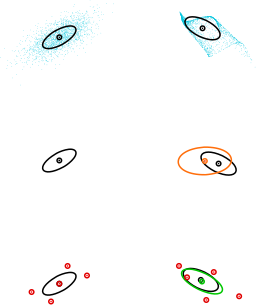
\includegraphics[width=\textwidth]{Figures/unscented_transform}} at (0pt,0pt);
    
    \node [label={right:Monte Carlo Simulation}] (a) at (-6, 7.3) {};
    \node [label={right:Linearisation}] (a) at (-6, 2.5) {};
    \node [label={right:Unscented Transformation}] (a) at (-6, -2.3) {};
    
    \node [] (b) at (-1, 5.2) (1) {};
    \node [] (c) at (2, 5.2) (2) {};
    \draw [->, align=center] (1) -- node[] {$\bm{y}^{(i)} = \bm{g}\big(\bm{x}^{(i)}\big)$} (2);
    
    \node [] (b) at (-1.5, 4.5)  (3) {\small covariance};
    \node [] (b) at (-2.7, 5.4) (4) {};
    \draw [->] (3) -- node[] {} (4);
    
    \node [] (b) at (-2.3, 3.6)  (3) {\small mean};
    \node [] (b) at (-3.2, 5.4) (4) {};
    \draw [->] (3) -- node[] {} (4);
    
    \node [] (b) at (1.9, 4.5)  (3) {\small sample mean};
    \node [] (b) at (3.5, 5.8) (4) {};
    \draw [->] (3) -- node[] {} (4);
    
    \node [] (b) at (3.1, 3.6)  (3) {\small sample covariance};
    \node [] (b) at (3.5, 5.4) (4) {};
    \draw [->] (3) -- node[] {} (4);
    
    \node [] (b) at (-6, 3)  (3) {};
    \node [] (b) at (6, 3) (4) {};
    \draw [dashed] (3) -- node[] {} (4);
    
    %%
    
    \node [] (b) at (-1, -0.5) (1) {};
    \node [] (c) at (2, -0.5) (2) {};
    \draw [->, align=left] (1) -- node[] {$\hat{\bm{y}} = \bm{g}(\bar{\bm{x}})$} (2);
    
    \node [] (b) at (4, 1.8) (3) {$\bm{P}_{\bm{y}} = \bm{G}^{[1]} \bm{P}_{\bm{x}} {\bm{G}^{[1]}}^T$};
    \node [] (b) at (4, 0.3) (4) {};
    \draw [->] (3) -- node[] {} (4);
    
    \node [] (b) at (-6, -1.8) (3) {};
    \node [] (b) at (6, -1.8) (4) {};
    \draw [dashed] (3) -- node[] {} (4);
    
    \node [] (b) at (2, 0.5) (3) {$\hat{\bm{y}}$};
    \node [] (b) at (3.5, -0.4) (4) {};
    \draw [->] (3) -- node[] {} (4);
    
    %%
    
    \node [] (b) at (-4, -4)  (3) {\small sigma points $\mathcal{X}_i$};
    \node [] (b) at (-2.8, -5.2) (4) {};
    \node [] (b) at (-4.5, -6.3) (5) {};
    \draw [->] (3) -- node[] {} (4);
    \draw [->] (3) -- node[] {} (5);
    
    \node [] (b) at (-1, -6) (1) {};
    \node [] (c) at (2, -6) (2) {};
    \draw [->, align=left] (1) -- node[] {$\mathcal{Y}_i = \bm{g}(\mathcal{X}_i)$} (2);
    
    \node [] (b) at (2.0, -3.2) (3) {$\bm{P}_{\bm{y}} \approx \sum^{2n}_{i = 0} W_i^{(c)} \big(\mathcal{Y}_i-\bar{\bm{y}}\big)\big(\mathcal{Y}_i-\bar{\bm{y}}\big)^T$};
    \node [] (b) at (2.7, -5.4) (4) {};
    \draw [->] (3) -- node[] {} (4);
    
    \node [] (b) at (4.3, -4.0) (3) {$\bar{\bm{y}} \approx \sum^{2n}_{i = 0} W_i^{(m)} \mathcal{Y}_i$};
    \node [] (b) at (3.5, -5.9) (4) {};
    \draw [->] (3) -- node[] {} (4);
    
\end{tikzpicture}
\caption[The unscented transformation in comparison with Monte Carlo simulation and linearisation about the mean.]{The unscented transformation in comparison with Monte Carlo sampling and linearisation about the mean \cite{wan2001unscented}. Above, a cloud $\big\{\bm{x}^{(i)}\big\}_{i=1}^N$ of $N = 200$ samples drawn from a two-dimensional Gaussian distribution is propagated individually through a highly non-linear function $\bm{g}$. After the transformation the empirical sample mean and covariance is computed, respectively. In the middle, the mean $\bar{\bm{x}}$ is propagated through $\bm{g}$ to obtain an estimate $\hat{\bm{y}}$ of the true mean $\bar{\bm{y}}$, and the covariance is approximated through a linearisation of $\bm{g}$ about $\bar{\bm{x}}$, using its Jacobian evaluated at $\bar{\bm{x}}$, which is denoted by $\bm{G}^{[1]}$. Below, the set of sigma points $\big\{\mathcal{X}_i\big\}_{i=1}^5$ capturing the true mean and covariance of the distribution of $\bm{x}$ are transformed independently and the mean and covariance is estimated, respectively. As can be seen, the result of the unscented transformation approximates the true mean and covariance better than the linearisation approach.}
	\label{fig:unscented_transform}
\end{figure}

In order to compute an estimate of the mean and covariance of an $m$-dimensional random variable $\bm{y}$, which is related to $\bm{x}$ by a non-linear transformation $\bm{g}: \mathbb{R}^{n} \rightarrow \mathbb{R}^{m}$, so that
 
\begin{equation}
  \bm{y} = \bm{g}(\bm{x})\,,
\end{equation}

\noindent
the sigma points $\mathcal{X}_i \in \bm{\mathcal{X}}$ are independently propagated through $\bm{g}$,

\begin{equation}
  \mathcal{Y}_i = \bm{g}\big(\mathcal{X}_i\big), \quad i \in \{0, \dots, 2n\}\,,
\end{equation}

\noindent
 to obtain a set $\bm{\mathcal{Y}}$ of transformed sigma points $\mathcal{Y}_i$.
 
 The mean $\bar{\bm{y}}$ and the covariance $\bm{P}_{\bm{y}}$ of the random variable $\bm{y}$ are approximated as the weighted sample mean and covariance of the posterior sigma points, respectively,

\begin{equation}
  \bar{\bm{y}} \approx \sum^{2n}_{i = 0} W_i^{(m)} \mathcal{Y}_i\,,
\end{equation}

\begin{equation}
  \bm{P}_{\bm{y}} \approx \sum^{2n}_{i = 0} W_i^{(c)} \big(\mathcal{Y}_i-\bar{\bm{y}}\big)\big(\mathcal{Y}_i-\bar{\bm{y}}\big)^T\,.
\end{equation}

\noindent
The weights for the mean, $W_i^{(m)}$, and for the covariance, $W_i^{(c)}$, are given by

\begin{equation}\label{eq:weights1}
  W^{(m)}_0 = \frac{\lambda}{n + \lambda} \,,
\end{equation}

\begin{equation}\label{eq:weights2}
  W^{(c)}_0 = \frac{\lambda}{n + \lambda} + (1- \alpha^2 + \beta) \,,
\end{equation}

\begin{equation}\label{eq:weights3}
  W_i^{(m)} = W_i^{(c)} = \frac{1}{2(n + \lambda)}, \quad i \in \{1, \dots, 2n\}\,.
\end{equation}

\noindent
The real parameter $\beta$ is used to incorporate information about the probability distribution of $\bm{x}$, where $\beta = 2$ is optimal if the distribution is Gaussian \cite{van2001unscented}.


Figure \ref{fig:unscented_transform} shows the unscented transformation for a two-dimensional random vector in comparison with Monto-Carlo sampling, which will be introduced in detail in Section \ref{sec:monte_carlo}, and the linearisation approach used by the extended Kalman filter. Note that only five sigma points are required to capture the mean and covariance of the distribution of $\bm{x}$. The mean and covariance of the independently transformed sigma points approximate the true mean and covariance up to the second order. \citeauthor{Julier96ageneral} mention the following significant advantages of the unscented transformation compared to the linearisation used in the EKF:

\begin{itemize}
	\item It is not necessary to compute Jacobians.
	\item In the prediction stage only standard linear algebra operations like matrix square roots, outer products, and matrix and vector summations are required.
	\item The number of computations, including an efficient computation of the matrix square root, scale with dimensions at the same rate as linearisation.
	\item Constraints can be seamlessly incorporated by applying them to each of the projected sigma points $\mathcal{Y}_i$.
\end{itemize}



\subsubsection{Unscented Kalman Filter Equations}

Given a discrete-time dynamic process and its ovservation governed by Equation \ref{eq:time_dynamical_system_plant_extended} and \ref{eq:time_dynamical_system_measurement_extended}, respectively, at each time step $k$ we compute the set of $2n_{\bm{x}}+1$ sigma points using the old posterior mean $\hat{\bm{x}}_{k-1}$ and covariance $\bm{P}_{k-1}$,

\begin{alignat}{3}
  \mathcal{X}_{0, k-1} &= \hat{\bm{x}}_{k-1}\,, \\
  \mathcal{X}_{i, k-1} &= \hat{\bm{x}}_{k-1} + \gamma \Big(\sqrt{ \bm{P}_{k-1}}\Big)_i, &&i \in \{1, \dots, n_{\bm{x}}\}\,, \\
  \mathcal{X}_{i, k-1} &= \hat{\bm{x}}_{k-1} - \gamma \Big(\sqrt{\bm{P}_{k-1}}\Big)_{i-n}, \quad &&i \in \{n_{\bm{x}}+1, \dots, 2n_{\bm{x}}\} \,,
\end{alignat}

\noindent
with

\begin{equation}
  \gamma = \sqrt{(n_{\bm{x}} + \lambda)}\,.
\end{equation}

\noindent
For the sake of brevity, in the following, the entire set of sigma points is denoted as

\begin{equation}
\begin{split}
  \bm{\mathcal{X}}_{k-1} &= \big\{\mathcal{X}_{0, k-1}, \mathcal{X}_{1, k-1}, \dots, \mathcal{X}_{2n_{\bm{x}}, k-1}\big\} \\
  &= \big\{\mathcal{X}_{0, k-1}\big\} \cup \big\{\mathcal{X}_{1, k-1}, \dots, \mathcal{X}_{n_{\bm{x}}, k-1}\big\} \\
  &\mathrel{\phantom{= \big\{\mathcal{X}_{0, k-1}\big\}}} \cup \, \big\{\mathcal{X}_{n_{\bm{x}} + 1, k-1}, \dots, \mathcal{X}_{2n_{\bm{x}}, k-1}\big\} \\
  &= \Big\{\hat{\bm{x}}_{k-1}, \quad \hat{\bm{x}}_{k-1} + \gamma \sqrt{\bm{P}_{k-1}}, \quad \hat{\bm{x}}_{k-1} - \gamma \sqrt{\bm{P}_{k-1}}\Big\}\,.
\end{split}
\end{equation}


Now we propagate the sigma points individually, taking into account the control input $\bm{u}_{k-1}$, to obtain the set of transformed sigma points $ \bm{\mathcal{X}}_{k|k-1}$. Again, more succinctly we write

\begin{equation}
  \bm{\mathcal{X}}_{k|k-1} = \bm{\phi}_{k-1}\big(\bm{\mathcal{X}}_{k-1}, \bm{u}_{k-1}\big)\,.
\end{equation}

\noindent
The a priori state estimate is computed as the weighted sample mean

\begin{equation}\label{eq:aprioriunscented}
  \hat{\bm{x}}_{k|k-1} = \sum^{2n}_{i = 0} W_i^{(m)} \mathcal{X}_{i, k|k-1}
\end{equation}

\noindent
and the a priori error covariance matrix as

\begin{equation}
  \bm{P}_{k|k-1} = \sum^{2n}_{i = 0} W_i^{(c)} \big(\mathcal{X}_{i, k|k-1} -\hat{\bm{x}}_{k|k-1}\big)\big(\mathcal{X}_{i, k|k-1}-\hat{\bm{x}}_{k|k-1}\big)^T + \bm{Q}_k\,.
\end{equation}

\noindent
where $\bm{Q}_k$ again denotes the process noise covariance matrix. Transforming the a priori sigma points individually using the measurement function $\bm{h}_{k}$ of Equation \ref{eq:time_dynamical_system_measurement_extended},

\begin{equation}
  \bm{\mathcal{Z}}_{k|k-1} = \bm{h}_{k}(\bm{\mathcal{X}}_{k|k-1})\,,
\end{equation}

\noindent
lets us compute the predicted measurement as the weighted sample mean of the transformed sigma points,

\begin{equation}\label{eq:innovation_covariance}
  \hat{\bm{z}}_{k|k-1} = \sum^{2n}_{i = 0} W_i^{(m)} \mathcal{Z}_{i, k|k-1}, \quad \mathcal{Z}_{i, k|k-1} \in \bm{\mathcal{Z}}_{k|k-1}\,.
\end{equation}


Now, we can compute the innovation covariance matrix

\begin{equation}\label{eq:cross_covariance}
  \bm{P}_{\tilde{\bm{z}}_k \tilde{\bm{z}}_k} = \sum^{2n}_{i = 0} W_i^{(c)} \big(\mathcal{Z}_{i, k|k-1} -\hat{\bm{z}}_{k|k-1}\big)\big(\mathcal{Z}_{i, k|k-1}-\hat{\bm{z}}_{k|k-1}\big)^T + \bm{R}_k
\end{equation}

\noindent
and the cross covariance matrix as

\begin{equation}\label{eq:crosscovunscented}
  \bm{P}_{\tilde{\bm{x}}_k \tilde{\bm{z}}_k} = \sum^{2n}_{i = 0} W_i^{(c)} \big(\mathcal{X}_{i, k|k-1} -\hat{\bm{x}}_{k|k-1}\big)\big(\mathcal{Z}_{i, k|k-1}-\hat{\bm{z}}_{k|k-1}\big)^T\,,
\end{equation}

\noindent
where $\bm{R}_k$ denotes the measurement noise covariance matrix. All weights $W_i$ in Equations \ref{eq:aprioriunscented}\,--\,\ref{eq:crosscovunscented} are computed according to Equations \ref{eq:weights1}\,--\,\ref{eq:weights3}. Given the covariance and cross covariance matrix, we can compute the Kalman gain as
 
\begin{equation}
  \mathcal{K}_k = \bm{P}_{\tilde{\bm{x}}_k \tilde{\bm{z}}_k}\bm{P}^{-1}_{\bm{z}_k\bm{z}_k}\,.
\end{equation}

As with the Kalman filter, the updated state estimate is the predicted state plus the innovation weighted by the Kalman gain,

\begin{equation}
  \hat{\bm{x}}_k = \hat{\bm{x}}_{k|k-1} + \mathcal{K}_k\big(\bm{z}_k - \hat{\bm{z}}_{k|k-1}\big)\,,
\end{equation}

\noindent
and the updated error covariance is the a priori error covariance minus the predicted measurement covariance, weighted by the Kalman gain,

\begin{equation}
  \bm{P}_k = \bm{P}_{k|k-1} - \mathcal{K}_k \bm{P}_{\tilde{\bm{z}}_k \tilde{\bm{z}}_k} \mathcal{K}^T_k\,.
\end{equation}


Figure \ref{fig:unscented_kalman_filter_cycle} shows the entire unscented Kalman filter cycle, illustrating the computation of sigma points and the `predict and correct' behaviour. Note that for now we assume additive zero-mean noise sources. In the next section, we will extend the UKF to arbitrary noise sources with Gaussian distributions.


\tikzstyle{block} = [draw, rectangle, thick, 
    minimum height=1.5cm, minimum width=11.6cm]
\tikzstyle{output} = [coordinate]

\begin{figure}
\centering
\begin{tikzpicture}[auto, rounded corners=1pt, node distance=5cm,>=latex']
    
\node [block, align=center] (init) {\emph{Initialisation} \\[3mm] 
	$\hat{\bm{x}}_{0} = \mathbb{E}[\bm{x}_{0}], \bm{P}_{0} = \mathbb{E}\big[(\bm{x}_{0} - \hat{\bm{x}}_{0}) (\bm{x}_{0} - \hat{\bm{x}}_{0})^T\big]$};
\node [block, align=center, below of=init, node distance=2.6cm] (sigma) {\emph{Calculation of sigma points} \\[3mm] 
	$\bm{\mathcal{X}}_{k-1} = \Big\{\hat{\bm{x}}_{k-1} \quad \hat{\bm{x}}_{k-1} + \gamma \sqrt{\bm{P}_{k-1}} \quad \hat{\bm{x}}_{k-1} - \gamma \sqrt{\bm{P}_{k-1}}\Big\}$};
\node [block, align=center, below of=sigma, node distance=4.9cm] (predict) {\emph{Time update} \\[3mm] 
	Propagate sigma points: \\ 
	$\bm{\mathcal{X}}_{k|k-1} = \bm{\phi}_{k-1}(\bm{\mathcal{X}}_{k-1}, \bm{u}_{k-1})$ \\[2mm]
	Compute a priori state estimate: \\ 
	$\hat{\bm{x}}_{k|k-1} = \sum^{2n}_{i = 0} W_i^{(m)} \mathcal{X}_{i, k|k-1}$ \\[2mm]
	Compute a priori error covariance: \\ 
	$\bm{P}_{k|k-1} = \sum^{2n}_{i = 0} W_i^{(c)} \big(\mathcal{X}_{i, k|k-1} -\hat{\bm{x}}_{k|k-1}\big)\big(\mathcal{X}_{i, k|k-1}-\hat{\bm{x}}_{k|k-1}\big)^T + \bm{Q}_k$ \\[2mm]
	Predict measurement: \\ 
	$\bm{\mathcal{Z}}_{k|k-1} = \bm{h}_{k}(\bm{\mathcal{X}}_{k|k-1})$ \\[1mm]
	$\hat{\bm{z}}_{k|k-1} = \sum^{2n}_{i = 0} W_i^{(m)} \mathcal{Z}_{i, k|k-1}$};
\node [block, align=center, below of=predict, node distance=7.3cm] (update) {\emph{Measurement update} \\[3mm] 
	Compute innovation and cross covariance matrix: \\ 
	$\bm{P}_{\tilde{\bm{z}}_k \tilde{\bm{z}}_k} = \sum^{2n}_{i = 0} W_i^{(c)} \big(\mathcal{Z}_{i, k|k-1} -\hat{\bm{z}}_{k|k-1}\big)\big(\mathcal{Z}_{i, k|k-1}-\hat{\bm{z}}_{k|k-1}\big)^T + \bm{R}_k$ \\[2mm]
	$\bm{P}_{\tilde{\bm{x}}_k \tilde{\bm{z}}_k} = \sum^{2n}_{i = 0} W_i^{(c)} \big(\mathcal{X}_{i, k|k-1} -\hat{\bm{x}}_{k|k-1}\big)\big(\mathcal{Z}_{i, k|k-1}-\hat{\bm{z}}_{k|k-1}\big)^T$ \\[2mm]
	Compute Kalman gain: \\
	$\mathcal{K}_k = \bm{P}_{\tilde{\bm{x}}_k \tilde{\bm{z}}_k}\bm{P}^{-1}_{\bm{z}_k\bm{z}_k}$ \\[2mm]
	Compute a posteriori state estimate: \\ $ \hat{\bm{x}}_k = \hat{\bm{x}}_{k|k-1} + \mathcal{K}_k(\bm{z}_k - \hat{\bm{z}}_{k|k-1})$ \\[2mm]
	Update error covariance: \\ $\bm{P}_k = \bm{P}_{k|k-1} - \mathcal{K}_k \bm{P}_{\tilde{\bm{z}}_k \tilde{\bm{z}}_k} \mathcal{K}^T_k$};
\node [output, below of=update, node distance=4.35cm, name=output] {Output};
\node [output, below of=update, node distance=3.8cm, name=help1] {};
\node [output, right of=help1, node distance=6.3cm, name=help2] {};
\node [output, below of=init, node distance=1.23cm, name=help4] {};
\node [output, right of=help4, node distance=6.3cm, name=help3] {};

\draw [draw,-stealth, thick, align=left] (init) -- (sigma);
\draw [draw,-stealth, thick, align=left] (sigma) -- (predict);
\draw [draw,-stealth, thick, align=left] (predict) -- (update);
\draw [draw,-stealth, thick, align=left] (update) -- node [label={left:Output}]{} (output);
\draw [draw,-stealth, thick] (help1) -- (help2) -- (help3) -- (help4);
\end{tikzpicture}
\caption[Operation cycle of the unscented Kalman filter for the additive zero-mean noise case.]{Operation cycle of the unscented Kalman filter for the additive zero-mean noise case, illustrating the computation of sigma points and its `predict and correct' behaviour.} \label{fig:unscented_kalman_filter_cycle}
\end{figure}


\subsubsection{Non-additive Noise}

In the case of non-additive non-zero mean process and measurement noise, the unscented transformation scheme is applied to the \emph{augmented state} $\bm{x}^a_k \in \mathbb{R}^{l}$, which is defined as the concatenation of the original state and the noise variables as

\begin{equation}
  \bm{x}^a_k = \Big[{\bm{x}_k}^T, {\bm{w}_k}^T, {\bm{v}_{k}}^T \Big]^T\,,
\end{equation}
 
 \noindent
 so that $l = n_{\bm{x}} + n_{\bm{w}} + n_{\bm{v}}$. The corresponding augmented error covariance matrix is given by
 
 \begin{equation}
  \bm{P}^a_k = \mathbb{E}\big[(\bm{x}^a_{k} - \hat{\bm{x}}^a_{k}) (\bm{x}^a_{k} - \hat{\bm{x}}^a_{k})^T\big] = \begin{bmatrix}
  \bm{P}_k & \bm{0} & \bm{0} \\
  \bm{0} & \bm{Q}_k & \bm{0} \\
  \bm{0} & \bm{0} & \bm{R}_k \\
\end{bmatrix}\,,
\end{equation}

\noindent
with

\begin{equation}
  \hat{\bm{x}}^a_k = \bigg[{\hat{\bm{x}}_k}^T, \mathbb{E}\big[{\bm{w}_k}\big]^T, \mathbb{E}\big[{\bm{v}_{k}}\big]^T \bigg]^T\,.
\end{equation}

\noindent
The zeros in bold typeface denote the zero matrix with respective dimension. Equally, every member $\mathcal{X}^{a}_{i, k}$ of the set $\bm{\mathcal{X}}^{a}_{k}$ of augmented sigma points is constituted of three vector-valued components,
 
\begin{equation}
   \mathcal{X}^{a}_{i, k} = \Big[{\mathcal{X}^{\bm{x}}_{i, k}}^T, {\mathcal{X}^{\bm{w}}_{i, k}}^T, {\mathcal{X}^{\bm{v}}_{i, k}}^T \Big]^T\,.
\end{equation}

\noindent
The vector space $\mathbb{R}^{n_{\bm{x}}}$ forms a linear subspace of $\mathbb{R}^{l}$. We denote the set of all sigma points $\mathcal{X}^{\bm{x}}_{i, k}$ belonging to this subspace with ${\bm{\mathcal{X}}^{\bm{x}}_{k}}$. Replacing the superscript $\bm{x}$ with $\bm{w}$ and $\bm{v}$, respectively, denotes the sigma points belonging to the subspaces spanned by the noise vectors, that is ${\bm{\mathcal{X}}^{\bm{w}}_{k}}$ and ${\bm{\mathcal{X}}^{\bm{v}}_{k}}$.

The augmented unscented Kalman filter algorithm is in structure similar to the that assuming additive noise in Figure \ref{fig:unscented_kalman_filter_cycle}, but it uses the augmented state to calculate sigma points, so that the set of sigma points is denoted as

\begin{equation}
  \bm{\mathcal{X}}^a_{k-1} = \Big\{\hat{\bm{x}}^a_{k-1}, \quad \hat{\bm{x}}^a_{k-1} + \gamma_a \sqrt{\bm{P}^a_{k-1}}, \quad \hat{\bm{x}}^a_{k-1} - \gamma_a \sqrt{\bm{P}^a_{k-1}}\Big\}\,,
\end{equation}

\noindent
with

\begin{equation}
  \gamma_a = \sqrt{(l + \lambda)}\,.
\end{equation}


Since we assume non-additive noise, we individually propagate the components of the sigma points that are associated with the state according to Equation \ref{eq:generic-state_dynamics},

\begin{equation}
  \bm{\mathcal{X}}^{\bm{x}}_{k|k-1} = \bm{\phi}_{k-1}\big(\bm{\mathcal{X}}^{\bm{x}}_{k-1}, \bm{u}_{k-1}, \bm{\mathcal{X}}^{\bm{w}}_{k-1}\big)\,,
\end{equation}

\noindent
and predict the measurement transforming the a priori sigma points according to Equation \ref{eq:generic-measurement},

\begin{equation}
  \bm{\mathcal{Z}}_{k|k-1} = \bm{h}_{k}\big(\bm{\mathcal{X}}^{\bm{x}}_{k|k-1}, \bm{\mathcal{X}}^{\bm{v}}_{k|k-1}\big)\,.
\end{equation}

\noindent
Figure \ref{fig:unscented_kalman_filter_cycle_non_addive} depicts the algorithm in its entirety, including the calculation of augmented sigma points and the predict and update operations that are carried out recursively at each time step.


\tikzstyle{block} = [draw, rectangle, thick, 
    minimum height=1.5cm, minimum width=10.65cm]
\tikzstyle{output} = [coordinate]

\begin{figure}
\centering
\begin{tikzpicture}[auto, rounded corners=1pt, node distance=5cm,>=latex']
    
\node [block, align=center] (init) {\emph{Initialisation} \\[3mm] 
	$\hat{\bm{x}}^a_0 = \bigg[{\hat{\bm{x}}_0}^T, \mathbb{E}\Big[{\bm{w}_0}^T\Big], \mathbb{E}\Big[{\bm{v}_{0}}^T\Big] \bigg]^T$ \\[2mm]
	$\bm{P}^a_{0} = \mathbb{E}\Big[\big(\bm{x}^a_{0} - \hat{\bm{x}}^a_{0}\big) \big(\bm{x}^a_{0} - \hat{\bm{x}}^a_{0}\big)^T\Big] = \begin{bsmallmatrix}
  \bm{P}_0 & \bm{0} & \bm{0} \\
  \bm{0} & \bm{Q}_0 & \bm{0} \\
  \bm{0} & \bm{0} & \bm{R}_0 \\
\end{bsmallmatrix}$};
\node [block, align=center, below of=init, node distance=3.4cm] (sigma) {\emph{Calculation of sigma points} \\[3mm] 
	$\bm{\mathcal{X}}^a_{k-1} = \Big\{\hat{\bm{x}}^a_{k-1}, \quad \hat{\bm{x}}^a_{k-1} + \gamma_a \sqrt{\bm{P}^a_{k-1}}, \quad \hat{\bm{x}}^a_{k-1} - \gamma_a \sqrt{\bm{P}^a_{k-1}}\Big\}$};
\node [block, align=center, below of=sigma, node distance=4.9cm] (predict) {\emph{Time update} \\[3mm] 
	Propagate sigma points: \\ 
	$\bm{\mathcal{X}}^{\bm{x}}_{k|k-1} = \bm{\phi}_{k-1}\big(\bm{\mathcal{X}}^{\bm{x}}_{k-1}, \bm{u}_{k-1}, \bm{\mathcal{X}}^{\bm{w}}_{k-1}\big)$ \\[2mm]
	Compute a priori state estimate: \\ 
	$\hat{\bm{x}}_{k|k-1} = \sum^{2l}_{i = 0} W_i^{(m)} \mathcal{X}^{\bm{x}}_{i, k|k-1}$ \\[2mm]
	Compute a priori error covariance: \\ 
	$\bm{P}_{k|k-1} = \sum^{2l}_{i = 0} W_i^{(c)} \big(\mathcal{X}^{\bm{x}}_{i, k|k-1} - \hat{\bm{x}}_{k|k-1}\big)\big(\mathcal{X}^{\bm{x}}_{i, k|k-1}-\hat{\bm{x}}_{k|k-1}\big)^T$ \\[2mm]
	Predict measurement: \\ 
	$\bm{\mathcal{Z}}_{k|k-1} = \bm{h}_{k}\big(\bm{\mathcal{X}}^{\bm{x}}_{k|k-1}, \bm{\mathcal{X}}^{\bm{v}}_{k|k-1}\big)$ \\[1mm]
	$\hat{\bm{z}}_{k|k-1} = \sum^{2l}_{i = 0} W_i^{(m)} \mathcal{Z}_{i, k|k-1}$};
\node [block, align=center, below of=predict, node distance=7.3cm] (update) {\emph{Measurement update} \\[3mm] 
	Compute innovation and cross covariance matrix: \\ 
	$\bm{P}_{\tilde{\bm{z}}_k \tilde{\bm{z}}_k} = \sum^{2l}_{i = 0} W_i^{(c)} \big(\mathcal{Z}_{i, k|k-1} -\hat{\bm{z}}_{k|k-1}\big)\big(\mathcal{Z}_{i, k|k-1}-\hat{\bm{z}}_{k|k-1}\big)^T$ \\[2mm]
	$\bm{P}_{\tilde{\bm{x}}_k \tilde{\bm{z}}_k} = \sum^{2l}_{i = 0} W_i^{(c)} \big(\mathcal{X}^{\bm{x}}_{i, k|k-1} -\hat{\bm{x}}_{k|k-1}\big)\big(\mathcal{Z}_{i, k|k-1}-\hat{\bm{z}}_{k|k-1}\big)^T$ \\[2mm]
	Compute Kalman gain: \\
	$\mathcal{K}_k = \bm{P}_{\tilde{\bm{x}}_k \tilde{\bm{z}}_k}\bm{P}^{-1}_{\bm{z}_k\bm{z}_k}$ \\[2mm]
	Compute a posteriori state estimate: \\ $ \hat{\bm{x}}_k = \hat{\bm{x}}_{k|k-1} + \mathcal{K}_k(\bm{z}_k - \hat{\bm{z}}_{k|k-1})$ \\[2mm]
	Update error covariance: \\ $\bm{P}_k = \bm{P}_{k|k-1} - \mathcal{K}_k \bm{P}_{\tilde{\bm{z}}_k \tilde{\bm{z}}_k} \mathcal{K}^T_k$};
\node [output, below of=update, node distance=4.4cm, name=output] {Output};
\node [output, below of=update, node distance=3.75cm, name=help1] {};
\node [output, right of=help1, node distance=5.8cm, name=help2] {};
\node [output, below of=init, node distance=2.05cm, name=help4] {};
\node [output, right of=help4, node distance=5.8cm, name=help3] {};

\draw [draw,-stealth, thick, align=left] (init) -- (sigma);
\draw [draw,-stealth, thick, align=left] (sigma) -- (predict);
\draw [draw,-stealth, thick, align=left] (predict) -- (update);
\draw [draw,-stealth, thick, align=left] (update) -- node [label={left:Output}]{} (output);
\draw [draw,-stealth, thick] (help1) -- (help2) -- (help3) -- (help4);
\end{tikzpicture}
\caption[Operation cycle of the unscented Kalman filter for the non-additive non-zero-mean noise case.]{Operation cycle of the unscented Kalman filter for the non-additive non-zero-mean noise case, illustrating the computation of sigma points and its `predict and correct' behaviour.} \label{fig:unscented_kalman_filter_cycle_non_addive}
\end{figure}

\section{Sequential Monte Carlo Simulation}\label{sec:monte_carlo}

If the assumptions of the Kalman filter hold, that is a linear process and measurement model and Gaussian distributions, then no other algorithm can outperform it \cite{gaussian_bayesian_tracking2002}. Real-life problems, however, may not always be described sufficiently accurate by linear-Gaussian models. \emph{Sequential Monte Carlo} (SMC) methods are a general simulation-based approach that essentially converts the intractable integrals of the Bayesian framework into tractable, finite sums, which converge to the exact solution in the limit. In contrast to the Kalman filtering methods above, they are not subject to any linearity or Gaussianity constraints on the model and entail appealing convergence properties \cite{doucet1998sequential}. These benefits, in turn, come along with increased computational cost.

If a sufficiently large number of samples drawn from the desired posterior distribution of the Bayesian framework is available, it is straightforward to approximate the intractable integrals appearing in Equations \ref{eq:chapman_kolmogorov} and \ref{eq:updated_posterior} in Section \ref{sec:bayesian_estimation}. In \emph{perfect Monte Carlo sampling} we assume that we are able to simulate  $N$ independent and identically distributed random samples $\bm{x}^{(i)}_k$, drawn from the posterior distribution $p(\bm{x}_k\,|\,\bm{Z}_{k}, \bm{U}_{k-1})$. These random samples are also called \emph{particles}. Each particle $\bm{x}^{(i)}_k$ is a concrete instantiation of the state at time $k$. That is, each particle represents a possible hypothesis as to what the true state of the system may be. An empirical estimate of the posterior distribution can then be computed as

\begin{equation}\label{eq:approximated_posterior}
  p(\bm{x}_k\,|\,\bm{Z}_{k}, \bm{U}_{k-1}) \approx \frac{1}{N} \sum^N_{i = 1} \delta\big(\bm{x}_{k} - \bm{x}^{(i)}_k \big) \,,
\end{equation}

\noindent
where $\delta\big(\bm{x}_{k} - \bm{x}^{(i)}_k\big)$ denotes the Dirac delta mass located in $\bm{x}^{(i)}_k$. Additionally, any expectation of the form

\begin{equation}\label{eq:expectations}
  \mathbb{E}_{p(\bm{x}_k\,|\,\bm{Z}_{k}, \bm{U}_{k-1})}\big[f(\bm{x}_k)\big] = \int f(\bm{x}_k) p(\bm{x}_k\,|\,\bm{Z}_{k}, \bm{U}_{k-1}) d\bm{x}_k
\end{equation}

\noindent
can be approximated as

\begin{equation}\label{eq:approximated_expectation}
\begin{split}
  \mathbb{E}_{p(\bm{x}_k\,|\,\bm{Z}_{k}, \bm{U}_{k-1})}\big[f(\bm{x}_k)\big] &\approx \hat{\mathbb{E}}_{p(\bm{x}_k\,|\,\bm{Z}_{k}, \bm{U}_{k-1})}\big[f(\bm{x}_k)\big] \\
  &= \frac{1}{N} \sum^N_{i = 1} f\Big(\bm{x}^{(i)}_k\Big) \,.
\end{split}
\end{equation}

%Figure \ref{fig:unscented_transform} illustrates Monte Carlo Sampling. The posterior mean and covariance is estimated by substituting $\bm{y}$ for $\bm{x}_k$ in Equation \ref{eq:approximated_expectation}. With $f(\bm{y}) = \bm{y}$ and $f(\bm{y}) = (\bm{y} - \hat{\bm{y}}) (\bm{y} - \hat{\bm{y}})^T$, respectively, this yields the sample mean
%
%\begin{equation}
%  \hat{\bm{y}} = \hat{\mathbb{E}}_{p(\bm{y}\,|\,\bm{x})}[\bm{y}] = \frac{1}{N} \sum^N_{i = 1} \bm{y}^{(i)}
%\end{equation}
%
%\noindent
%and the sample covariance
%
%\begin{equation}
%  \bm{P}_{\bm{y}} = \hat{\mathbb{E}}_{p(\bm{y}\,|\,\bm{x})}\Big[(\bm{y} - \hat{\bm{y}}) (\bm{y} - \hat{\bm{y}})^T\Big] = \sum^N_{i = 1} \big(\bm{y}^{(i)} - \hat{\bm{y}}\big) \big(\bm{y}^{(i)} - \hat{\bm{y}}\big)^T \,.
%\end{equation}


As opposed to most deterministic numerical methods, the estimation accuracy is independent of the dimensionality of the state space. According to the law of large numbers, for $N\to\infty$ the estimated expectation almost surely converges to the true expectation, 

\begin{equation}
  \hat{\mathbb{E}}_{p(\bm{x}_k\,|\,\bm{Z}_{k}, \bm{U}_{k-1})}\big[f(\bm{x}_k)\big] \xrightarrow{\mathrm{a.s.}} \mathbb{E}_{p(\bm{x}_k\,|\,\bm{Z}_{k}, \bm{U}_{k-1})}\big[f(\bm{x}_k)\big], \quad \textrm{for}\: N\to\infty\,.
\end{equation}


\subsection{Sequential Importance Sampling}\label{sec:importance_sampling}

Since it is rarely possible to sample directly from the posterior distribution, \emph{importance sampling} is used, which refers to sampling from an alternative distribution \cite{geweke1989bayesian}. This easy-to-sample importance sampling distribution is also called \emph{proposal distribution}. Expanding Equation \ref{eq:expectations} with an arbitrary proposal distribution $\pi(\bm{x}_k\,|\,\bm{Z}_{k}, \bm{U}_{k-1})$ and applying Bayes' theorem yields

\begin{equation}\label{eq:importance_sampling}
\begin{split}
  \mathbb{E}_{p(\bm{x}_k\,|\,\bm{Z}_{k}, \bm{U}_{k-1})}\big[f(\bm{x}_k)\big] &= \int f(\bm{x}_k) \frac{p(\bm{x}_k\,|\,\bm{Z}_{k}, \bm{U}_{k-1})}{\pi(\bm{x}_k\,|\,\bm{Z}_{k}, \bm{U}_{k-1})}  \\
  &\mathrel{\phantom{iiiiiiiiiii}} \cdot \: \pi(\bm{x}_k\,|\,\bm{Z}_{k}, \bm{U}_{k-1}) d\bm{x}_k \\
  &= \int f(\bm{x}_k) \frac{p(\bm{Z}_k\,|\,\bm{x}_{k}, \bm{U}_{k-1}) p(\bm{x}_{k}\,|\,\bm{U}_{k-1})}{p(\bm{Z}_{k}\,|\,\bm{U}_{k-1}) \pi(\bm{x}_k\,|\,\bm{Z}_{k}, \bm{U}_{k-1})} \\
  &\mathrel{\phantom{iiiiiiiiiii}} \cdot \: \pi(\bm{x}_k\,|\,\bm{Z}_{k}, \bm{U}_{k-1}) d\bm{x}_k \\
  &= \int f(\bm{x}_k) w_k(\bm{x}_k) p(\bm{Z}_k\,|\,\bm{U}_{k-1})^{-1} \\
  &\mathrel{\phantom{iiiiiiiiiii}} \cdot \: \pi(\bm{x}_k\,|\,\bm{Z}_{k}, \bm{U}_{k-1}) d\bm{x}_k\,,
\end{split}
\end{equation}

\noindent
with the \emph{importance weight}

\begin{equation}\label{eq:importance_weight}
  w_k(\bm{x}_k) = \frac{p(\bm{Z}_k\,|\,\bm{x}_{k}, \bm{U}_{k-1}) p(\bm{x}_{k}\,|\,\bm{U}_{k-1})}{\pi(\bm{x}_k\,|\,\bm{Z}_{k}, \bm{U}_{k-1})} \,.
\end{equation}

\noindent
The unknown normalising distribution $p(\bm{Z}_k\,|\,\bm{U}_{k-1})$ can be written as

\begin{equation}
  p(\bm{Z}_k\,|\,\bm{U}_{k-1}) = \int p(\bm{Z}_k\,|\,\bm{x}_{k}, \bm{U}_{k-1}) p(\bm{x}_{k}\,|\,\bm{U}_{k-1}) d\bm{x}_{k} \,.
\end{equation}

\noindent
Multiplying the integrand with $\frac{\pi(\bm{x}_k\,|\,\bm{Z}_{k}, \bm{U}_{k-1})}{\pi(\bm{x}_k\,|\,\bm{Z}_{k}, \bm{U}_{k-1})}$ and substituting with the left side of Equation \ref{eq:importance_weight}, we have

\begin{equation}
  p(\bm{Z}_k\,|\,\bm{U}_{k-1}) = \int w_k(\bm{x}_k) \pi(\bm{x}_k\,|\,\bm{Z}_{k}, \bm{U}_{k-1})d\bm{x}_{k} \,.
\end{equation}

\noindent
Plugging the result back into Equation \ref{eq:importance_sampling} yields

\begin{equation}
\begin{split}
  \mathbb{E}_{p(\bm{x}_k\,|\,\bm{Z}_{k}, \bm{U}_{k-1})}\big[f(\bm{x}_k)\big] &= \frac{\int f(\bm{x}_k) w_k(\bm{x}_k) \pi(\bm{x}_k\,|\,\bm{Z}_{k}, \bm{U}_{k-1}) d\bm{x}_k}{\int w_k(\bm{x}_k) \pi(\bm{x}_k\,|\,\bm{Z}_{k}, \bm{U}_{k-1})d\bm{x}_{k}} \\
  &= \frac{\mathbb{E}_{\pi(\bm{x}_k\,|\,\bm{Z}_{k}, \bm{U}_{k-1})}\big[w_k(\bm{x}_k)f(\bm{x}_k)\big]}{\mathbb{E}_{\pi(\bm{x}_k\,|\,\bm{Z}_{k}, \bm{U}_{k-1})}\big[w_k(\bm{x}_k)\big]} \\
  &\approx \frac{\frac{1}{N} \sum^N_{i = 1} w_k\Big(\hat{\bm{x}}^{(i)}_k\Big)f\Big(\hat{\bm{x}}^{(i)}_k\Big)}{\frac{1}{N} \sum^N_{i = 1} w_k\Big(\hat{\bm{x}}^{(i)}_k\Big)} \\
  &= \frac{1}{N} \sum^N_{i = 1} \tilde{w}_k\Big(\hat{\bm{x}}^{(i)}_k\Big)f\Big(\hat{\bm{x}}^{(i)}_k\Big)
  \,,
\end{split}
\end{equation}

\noindent
where $\hat{\bm{x}}^{(i)}_k$ denotes the $i$-th of $N$ samples drawn from $\pi(\bm{x}_k\,|\,\bm{Z}_{k}, \bm{U}_{k-1})$ and the normalised importance weights $\tilde{w}_k\Big(\hat{\bm{x}}^{(i)}_k\Big)$ are given by 

\begin{equation}
  \tilde{w}_k\Big(\hat{\bm{x}}^{(i)}_k\Big) = \frac{w_k\Big(\hat{\bm{x}}^{(i)}_k\Big)}{\sum^N_{i = 1} w_k\Big(\hat{\bm{x}}^{(i)}_k\Big)} \,.
\end{equation}


It follows that any expectation of the form given by Equation \ref{eq:expectations} can be estimated using weighted samples $\hat{\bm{x}}^{(i)}_k$ drawn from the proposal distribution $\pi(\bm{x}_k\,|\,\bm{Z}_{k}, \bm{U}_{k-1})$. As it involves a ratio of two other estimates, this estimate is biased. However, given that the support of the proposal distribution includes the support of the posterior distribution $p(\bm{x}_k\,|\,\bm{Z}_{k}, \bm{U}_{k-1})$, that is the following condition is satisfied: $\pi(\bm{x}_k\,|\,\bm{Z}_{k}, \bm{U}_{k-1}) \neq 0$ for any $\bm{x}_k$ for which $p(\bm{x}_k\,|\,\bm{Z}_{k}, \bm{U}_{k-1}) \neq 0$, it is shown that this estimate is asymptotically unbiased \cite{doucet1998sequential}. Given samples drawn from the proposal distribution, the posterior distribution is approximated by the weighted point-mass estimate

\begin{equation}\label{eq:weighted_empirical_distribution}
  p(\bm{x}_k\,|\,\bm{Z}_{k}, \bm{U}_{k-1}) \approx \sum^N_{i = 1} \tilde{w}_k\Big(\hat{\bm{x}}^{(i)}_k\Big) \delta\Big(\bm{x}_{k} - \hat{\bm{x}}^{(i)}_k \Big) \,.
\end{equation}

Under the premise of the state space assumptions mentioned in Section \ref{sec:bayesian_estimation}, that is Markovianess and observational independence given the state, as shown in \cite{doucet2001introduction}, a recursive estimate for the importance weights may be obtained as

\begin{equation}\label{eq:recursive_weights}
  \tilde{w}_k\Big(\hat{\bm{x}}^{(i)}_k\Big) = \tilde{w}_{k-1}\Big(\hat{\bm{x}}^{(i)}_{k-1} \Big) \frac{p\big(\bm{z}_k\,|\,\hat{\bm{x}}^{(i)}_k\big) p\big(\hat{\bm{x}}^{(i)}_k\,|\,\hat{\bm{x}}^{(i)}_{k-1}, \bm{u}_{k-1}\big)}{\pi\big(\hat{\bm{x}}^{(i)}_k\,|\,\hat{\bm{X}}^{(i)}_{k-1}, \bm{U}_{k-1}, \bm{Z}_{k}\big)} \,.
\end{equation}

\noindent
This variant of importance sampling is called \emph{sequential importance sampling} (SIS), referring to its recursive nature. As it is clear that the weights $w_k\big(\hat{\bm{x}}^{(i)}_k\big)$ and normalised weights $\tilde{w}_k\big(\hat{\bm{x}}^{(i)}_k\big)$ are a function of the particles $\hat{\bm{x}}^{(i)}_k$, respectively, we will use a more succinct notation and from now on write $w^{(i)}_k$ and $\tilde{w}^{(i)}_k$ instead.


\subsection{Sequential Importance Resampling}\label{sec:importance_resampling}

\begin{figure}
\centering
\begin{tikzpicture}[scale=1.0, auto, thick, node distance=3cm,>=latex']
    \pgftext{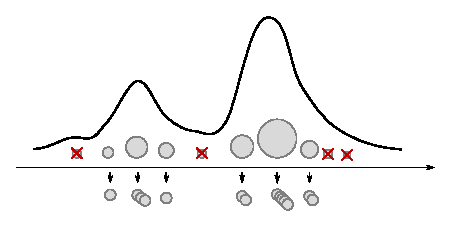
\includegraphics[width=0.80\textwidth]{Figures/resampling}} at (0, 0);
    
    %\node [] (a) at (0.3, -2.6) {$N$};
        
\end{tikzpicture}
\caption[Resampling: replacing the weighted empirical distribution by an unweighted distribution.]{Resampling: replacing the weighted empirical distribution by an unweighted distribution \cite{garciabayes}. Before resampling, the size of the samples represents their respective importance weight. Samples with low weights are likely to be eliminated, whereas samples with higher weights are likely to be reproduced.}
	\label{fig:resampling}
\end{figure}


A serious limitation of sequential importance sampling is that it degenerates with time. In fact, it is shown in \cite{kong1994sequential} that SIS is guaranteed to fail for large $k$, as the distribution of the importance weights becomes more and more skewed \cite{merwe2000scented}. After a few time steps, the majority of particles have a numerically insignificant importance weight, while the weight of one particle tends to one, which is effectively equal to removing the samples from the sample set. The consequence is that the posterior distribution is not adequately represented by the few remaining effective samples.

An additional selection step called \emph{sequential importance resampling} (SIR), or simply \emph{resampling}, partially mitigates this problem. Introduced in \cite{gordon1993novel}, the rationale behind the resampling idea is to eliminate the particles with low importance weight and instead multiply particles having high weight. Therefore, the resampling procedure reflects the Darwinian idea of \emph{survival of the fittest} and is illustrated for one dimension in Figure \ref{fig:resampling}. 

Formally, resampling is carried out by replacing the weighted empirical distribution in Equation \ref{eq:weighted_empirical_distribution} by an unweighted distribution

\begin{equation}
  p(\bm{x}_k\,|\,\bm{Z}_{k}, \bm{U}_{k-1}) = \frac{1}{N} \sum^N_{i = 1} N_k^{(i)}  \delta\Big(\bm{x}_{k} - \bm{x}^{(i)}_k \Big) \,,
\end{equation}

\noindent
where $N_k^{(i)}$ is the number of offsprings from particle $\hat{\bm{x}}^{(i)}_k$, such that the number of particles remains constant,

\begin{equation}
  \sum^N_{i = 1} N_k^{(i)} = N  \,.
\end{equation}

\begin{figure}
\centering
\begin{tikzpicture}[scale=1.0, auto, thick, node distance=3cm,>=latex']
    \pgftext{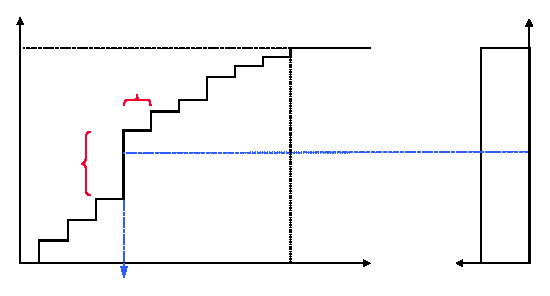
\includegraphics[width=0.80\textwidth]{Figures/weighted_mapping}} at (0, 0);
    
    \node [] (a) at (-4.0, 2.2) {CDF};
    \node [] (a) at (-5, 1.8) {$1$};
    \node [] (a) at (-5, -2.1) {$0$};
    \node [] (a) at (-4, -0.2) {$\tilde{w}^{(j)}_{k}$};
    \node [] (a) at (-2.51, 1.2) {$1$};
    \node [] (a) at (-2.75, -2.6) {$j$};
    \node [] (a) at (-4.4, -2.6) {$1$};
    \node [] (a) at (0.3, -2.6) {$N$};
    \node [] (a) at (4.2, -2.6) {$p(\cdot)$};
    \node [] (a) at (5, 1.8) {$1$};
    \node [] (a) at (5, -2.1) {$0$};
        
\end{tikzpicture}
\caption[A simple resampling scheme: multinomial resampling.]{Multinomial resampling \cite{merwe2000scented}. Depicted is the projection of a random sample from the continuous uniform distribution on the interval $[0, 1]$ onto the range of the cumulative distribution function (CDF), which is plotted over the sample numbers $1, \dots, N$. The intersection with the CDF is projected on the abscissa to obtain the sample number $j$, which is then used to select a sample from $\big\{\hat{\bm{x}}^{(j)}_k\big\}_{j=1}^N$.}
	\label{fig:weightes_measure_to_unweighted_measure}
\end{figure}

\subsubsection{Multinomial Resampling}

Employing the most popular resampling scheme termed \emph{multinomial resampling}, which was introduced in \cite{gordon1993novel}, the surviving particles are obtained by drawing $N$ samples $\bm{x}^{(i)}_k$ from the set $\big\{\hat{\bm{x}}^{(j)}_k\big\}_{j=1}^N$, whilst samples are chosen with a probability equal to their normalised importance weight. This yields the resampled set

\begin{equation}\label{eq:resampling}
 \big\{\bm{x}^{(i)}_k\big\}_{i=1}^N,\:\:\, \text{such that} \:\:\:\operatorname{Pr}\big(\bm{x}^{(i)}_k = \hat{\bm{x}}^{(j)}_k\big) = \tilde{w}^{(j)}_k, \quad i, j \in \{1, \dots, N\}\,,
 \end{equation}

\noindent
with equal weights, 

\begin{equation}\label{eq:resampling_weights}
  w^{(i)}_k = \frac{1}{N}, \quad i = 1, \dots, N \,.
\end{equation}


\noindent
The mapping from a weighted random measure to an unweighted random measure using a uniform distribution is illustrated in Figure \ref{fig:weightes_measure_to_unweighted_measure}. First, the cumulative distribution function (CDF) of the set $\big\{\hat{\bm{x}}^{(j)}_k\big\}_{j=1}^N$ is constructed. Then, a number from the continuous uniform distribution on the interval $[0, 1]$ is sampled and projected on the range of the CDF. The intersection is projected on the sample number, which is used to select the $j$-th sample from $\big\{\hat{\bm{x}}^{(j)}_k\big\}_{j=1}^N$.


\subsection{Importance of the Proposal Distribution}\label{sec:importance_proposal}

For a finite set of samples, the importance sampling method performs poorly if only a few particles are placed in regions where the desired posterior is large \cite{chen2003bayesian}. This makes the choice of the proposal distribution a critical design issue for SIS algorithms \cite{merwe2000scented, daum2005nonlinear}.  

An optimal proposal distribution may be defined as one that minimises the variance of the importance weights \cite{doucet2001particle}. Then, as shown analogously to the proof in \cite{5546308}, which does not consider a control input, the target distribution is given by

\begin{equation}\label{eq:optimal_proposal}
\begin{split}
  \pi_{\mathrm{opt}}\big(\bm{x}_k\,|\,\bm{X}^{(i)}_{k-1}, \bm{U}_{k-1}, \bm{Z}_{k}\big) &= p\big(\bm{x}_k\,|\,\bm{x}^{(i)}_{k-1}, \bm{u}_{k-1}, \bm{z}_{k}\big) \\
  &=  \frac{p\big(\bm{z}_k\,|\,\bm{x}_k\big) p\big(\bm{x}_k\,|\,\bm{x}^{(i)}_{k-1}, \bm{u}_{k-1}\big)}{p\big(\bm{z}_k\,|\,\bm{x}^{(i)}_{k-1}, \bm{u}_{k-1}\big)} \,.
  \end{split}
\end{equation}

\noindent
Plugging the result into Equation \ref{eq:recursive_weights} yields

\begin{equation}\label{eq:recursive_weights_minvar}
\begin{split}
  \tilde{w}_k &= \tilde{w}_{k-1} p\big(\bm{z}_k\,|\,\bm{x}^{(i)}_{k-1}, \bm{u}_{k-1}\big) \\
   &= \tilde{w}_{k-1} \int p\big(\bm{z}_k\,|\,\bm{x}_k\big) p\big(\bm{x}_k\,|\,\hat{\bm{x}}^{(i)}_{k-1}, \bm{u}_{k-1}\big) d\bm{x}_k \,.
\end{split}
\end{equation}

\noindent
However, this density suffers from the following two major drawbacks: it requires the ability to sample from $p\big(\bm{x}_k\,|\,\bm{x}^{(i)}_{k-1}, \bm{u}_{k-1}, \bm{z}_{k}\big)$ and to evaluate the integral in Equation \ref{eq:recursive_weights_minvar}, both of which may not be straightforward in practice \cite{gaussian_bayesian_tracking2002}. Therefore, it is desirable  to find an approximation of the optimal proposal distribution. In \cite{Salmond2006DRAFT}, \citeauthor{Salmond2006DRAFT} state the ``considerable scope for ingenuity in designing the importance density''. A popular method for devising a proposal distribution that approximates the optimal distribution given by Equation \ref{eq:optimal_proposal} is taking into account the latest measurement \cite{doucet1998sequential, pitt_auxiliary}, which we will elaborate on in detail in Section \ref{sec:unscented_particle}.



\section{Particle Filters}

In this section, we shall introduce a non-parametric filtering method known as the \emph{particle filter}. Relying in principle on the Monte Carlo method, particle filters can handle arbitrary multi-modal distributions. However, their computational cost is a monotonically increasing function of the estimation accuracy.


\subsection{The Generic Particle Filter}\label{sec:particle}

The generic particle filter is a Monte Carlo algorithm that matches the Bayesian framework. Starting the filter algorithm at time $k=0$, first, $N$ samples $\bm{x}^{(i)}_0$ from the initial state distribution $p(\bm{x}_0)$ are drawn,

\begin{equation}\label{eq:draw_initial_particles}
  \bm{x}^{(i)}_0 \sim p(\bm{x}_0), \quad i \in \{1, \dots, N\} \,,
\end{equation}

\noindent
and weighted equally as

\begin{equation}
  w^{(i)}_0 = \frac{1}{N}, \quad i \in \{1, \dots, N\} \,.
\end{equation}

\noindent
Then, the following steps are carried out recursively at every time step $k > 0$. We draw $N$ equally weighted samples $\hat{\bm{x}}^{(i)}_k$ from the proposal distribution $\pi\big(\bm{x}_k\,|\,\bm{X}^{(i)}_{k-1}, \bm{Z}_{k}, \bm{U}_{k-1}\big)$. The set of particles and their respective weights is denoted as


\begin{equation}
  \Big\{\big(\hat{\bm{x}}^{(i)}_{k}, N^{-1}\big)\Big\}_{i=1}^N, \quad \hat{\bm{x}}^{(i)}_k \sim \pi\big(\bm{x}_k\,|\,\bm{X}^{(i)}_{k-1}, \bm{Z}_{k}, \bm{U}_{k-1}\big)\,.
\end{equation}


In the light of the measurement $\bm{z}_k$, the importance weights $w^{(i)}_k$ are computed for each particle according to Equation \ref{eq:recursive_weights},

\begin{equation}\label{eq:weights_generic_particle}
   w^{(i)}_k = w^{(i)}_{k-1} \frac{p\big(\bm{z}_k\,|\,\hat{\bm{x}}^{(i)}_k\big) p\big(\hat{\bm{x}}^{(i)}_k\,|\,\bm{x}^{(i)}_{k-1}, \bm{u}_{k-1}\big)}{\pi\big(\hat{\bm{x}}^{(i)}_k\,|\,\bm{X}^{(i)}_{k-1}, \bm{Z}_{k}, \bm{U}_{k-1}\big)}, \quad i \in \{1, \dots, N\}\,.
\end{equation}

\noindent
Normalising yields

\begin{equation}
  \tilde{w}^{(i)}_k = w^{(i)}_{k} \Bigg[\sum^N_{j = 1} w^{(j)}_k\Bigg]^{-1}, \quad i \in \{1, \dots, N\}\,.
\end{equation}

\noindent
Now, the set of particles is resampled according to Equation \ref{eq:resampling} and the weights are set equally according to Equation \ref{eq:resampling_weights}.


The output of the filter is given by a set of $N$ equally weighted particles $\bm{x}^{(i)}_k$ that can be used to approximate the posterior distribution, according to Equation \ref{eq:approximated_posterior}, and the expectations under it, according to Equation \ref{eq:approximated_expectation}. Often, the estimate of the conditional mean

\begin{equation}\label{eq:empirical_mean}
  \hat{\bm{x}}_k = \tilde{\mathbb{E}}_{p(\bm{x}_k\,|\,\bm{Z}_{k}, \bm{U}_{k-1})}\big[\bm{x}_k\big] = \frac{1}{N} \sum^N_{i = 1} \bm{x}^{(i)}_k \,,
\end{equation}

\noindent
which represents the minimum mean-squared error estimate of the current state, and the covariance

\begin{equation}\label{eq:empirical_cov}
\begin{split}
  \bm{P}_k &= \tilde{\mathbb{E}}_{p(\bm{x}_k\,|\,\bm{Z}_{k}, \bm{U}_{k-1})}\Big[\big(\bm{x}_k - \hat{\bm{x}}_{k}\big) \big(\bm{x}_k - \hat{\bm{x}}_{k}\big)^T\Big] \\
  &= \sum^N_{i = 1} \big(\bm{x}^{(i)}_k - \hat{\bm{x}}_{k}\big) \big(\bm{x}^{(i)}_k - \hat{\bm{x}}_{k}\big)^T \,,
\end{split}
\end{equation}


\noindent
are the quantities of particular interest. The algorithm of the generic particle filter is depicted in Figure \ref{fig:particle_filter_cycle}, illustrating the importance sampling and resampling step.

\tikzstyle{block} = [draw, rectangle, thick, 
    minimum height=1.5cm, minimum width=11cm]
\tikzstyle{output} = [coordinate]

\begin{figure}
\centering
\begin{tikzpicture}[auto, rounded corners=1pt, node distance=5cm,>=latex']
    
\node [block, align=center] (init) {\emph{Initialisation} \\[3mm] 
	Draw $N$ samples $\bm{x}^{(i)}_0$ from the initial state distribution: \\[2mm]
	$\Big\{\big(\bm{x}^{(i)}_{0}, N^{-1}\big)\Big\}_{i=1}^N, \quad \bm{x}^{(i)}_0 \sim p(\bm{x}_0)$};
\node [block, align=center, below of=init, node distance=4.7cm] (predict) {\emph{Importance sampling step} \\[3mm] 
	Draw $N$ samples $\hat{\bm{x}}^{(i)}_k$ from the proposal distribution: \\
	$\Big\{\big(\hat{\bm{x}}^{(i)}_{k}, N^{-1}\big)\Big\}_{i=1}^N, \quad \hat{\bm{x}}^{(i)}_k \sim \pi\big(\bm{x}_k\,|\,\bm{X}^{(i)}_{k-1}, \bm{Z}_{k}, \bm{U}_{k-1}\big)$ \\[2mm]
	Evaluate importance weights: \\
	$w^{(i)}_k = w^{(i)}_{k-1} \frac{p\big(\bm{z}_k\,|\,\hat{\bm{x}}^{(i)}_k\big) p\big(\hat{\bm{x}}^{(i)}_k\,|\,\bm{x}^{(i)}_{k-1}, \bm{u}_{k-1}\big)}{\pi\big(\hat{\bm{x}}^{(i)}_k\,|\,\bm{X}^{(i)}_{k-1}, \bm{Z}_{k}, \bm{U}_{k-1}\big)}, \quad i \in \{1, \dots, N\}$ \\[2mm]
	Normalise importance weights: \\
	$\tilde{w}^{(i)}_k = w^{(i)}_{k} \Big[\sum^N_{j = 1} w^{(j)}_k\Big]^{-1}, \quad i \in \{1, \dots, N\}$};
	\node [block, align=center, below of=predict, node distance=4.6cm] (update) {\emph{Resampling step} \\[3mm] 
	Draw $N$ samples $\bm{x}^{(i)}_{k}$ from the set $\Big\{\big(\hat{\bm{x}}^{(j)}_{k}, \tilde{w}^{(j)}_{k}\big)\Big\}_{j=1}^N$: \\[1mm]
	$\Big\{\big(\bm{x}^{(i)}_{k}, N^{-1}\big)\Big\}_{i=1}^N, \quad \operatorname{Pr}\big(\bm{x}^{(i)}_k = \hat{\bm{x}}^{(j)}_k\big) = \tilde{w}^{(j)}_k, \quad i,j \in \{1, \dots, N\}$};
	\node [block, align=center, below of=update, node distance=3.5cm] (outputblock) {\emph{Recombine particles} \\[3mm] 
	Compute conditional mean: \\
	$\hat{\bm{x}}_k = \tilde{\mathbb{E}}_{p(\bm{x}_k\,|\,\bm{Z}_{k}, \bm{U}_{k-1})}\big[\bm{x}_k\big] = \frac{1}{N} \sum^N_{i = 1} \bm{x}^{(i)}_k$ \\[2mm]
	Compute covariance: \\
	$\bm{P}_k = \sum^N_{i = 1} \big(\bm{x}^{(i)}_k - \hat{\bm{x}}_{k}\big) \big(\bm{x}^{(i)}_k - \hat{\bm{x}}_{k}\big)^T$};

\node [output, below of=outputblock, node distance=2.8cm, name=output] {Output};
\node [output, below of=outputblock, node distance=2.2cm, name=help1] {};
\node [output, right of=help1, node distance=6cm, name=help2] {};
\node [output, below of=init, node distance=1.6cm, name=help4] {};
\node [output, right of=help4, node distance=6cm, name=help3] {};

\draw [draw,-stealth, thick, align=left] (init) -- (predict);
\draw [draw,-stealth, thick, align=left] (predict) -- (update);
\draw [draw,-stealth, thick, align=left] (update) -- (outputblock);
\draw [draw,-stealth, thick, align=left] (outputblock) -- node [label={left:Output}]{} (output);
\draw [draw,-stealth, thick] (help1) -- (help2) -- (help3) -- (help4);
\end{tikzpicture}
\caption[Operation cycle of the generic particle filter.]{Operation cycle of the generic particle filter, illustrating the importance sampling and resampling step. Finally, the particles are recombined to obtain the minimum mean-squared error estimate and the corresponding covariance.} \label{fig:particle_filter_cycle}
\end{figure}



\subsection{The Bootstrap Filter}\label{sec:bootstrap_filter}

Although many authors have recognised the importance of the proposal distribution for a successful application of SIS \cite{doucet2000sequential, liu1998sequential, lenser2000sensor}, the transition prior probability distribution  $p(\bm{x}_k\,|\,\bm{x}_{k-1}, \bm{u}_{k-1})$ is often used as importance function \cite{avitzour1995stochastic, gordon1993novel, beadle1997fast, isard1996contour, kitagawa1996monte}. Filters using the transition prior as proposal distribution are commonly known as \emph{bootstrap filter}. The transition prior is easy to sample from and, as a result of it not incorporating the most recent observation, it is usually easier to implement \cite{doucet1998sequential, liu1998sequential, berzuini1997dynamic}. In the case of an additive Gaussian process noise model, the transition prior is simply

\begin{equation}\label{eq:weights_recursive_simplified}
  p(\bm{x}_k\,|\,\bm{x}_{k-1}, \bm{u}_{k-1}) = \mathcal{N}\big(\bm{\phi}_{k-1}(\bm{x}_{k-1}, \bm{u}_{k-1}, 0), \bm{Q}_{k-1}\big)\,.
\end{equation}


In the importance sampling step of the bootstrap filter, each of the particles is propagated through the system model according to Equation \ref{eq:generic-state_dynamics}, 

\begin{equation}\label{eq:propagate_particles}
  \hat{\bm{x}}^{(i)}_k = \bm{\phi}_{k-1}\big(\bm{x}^{(i)}_{k-1}, \bm{u}_{k-1}, \bm{w}^{(i)}_{k-1}\big), \quad k > 0,  \quad i \in \{1, \dots, N\}\,.
\end{equation}

\noindent
where $\bm{w}^{(i)}_{k-1}$ represents a sample drawn from the system noise distribution. Adding this noise sample creates variety in the set of hypotheses $\Big\{\big(\hat{\bm{x}}^{(i)}_{k}, N^{-1}\big)\Big\}_{i=1}^N$. Note that this step is equivalent to sampling from the prior distribution, as

\begin{equation}
  \hat{\bm{x}}^{(i)}_k \sim p\big(\bm{x}_k\,|\,\bm{x}^{(i)}_{k-1}, \bm{u}_{k-1}\big), \quad k > 0,  \quad i \in \{1, \dots, N\}\,.
\end{equation}


Now, in the light of the measurement $\bm{z}_k$, the importance weights $w^{(i)}_k$ are computed for each particle. When using the transition prior as proposal distribution, with

\begin{equation}
  \pi\big(\bm{x}_k\,|\,\bm{X}^{(i)}_{k-1}, \bm{Z}_{k}, \bm{U}_{k-1}\big) = p\big(\bm{x}_k\,|\,\bm{x}^{(i)}_{k-1}, \bm{u}_{k-1}\big)\,,
\end{equation}

\noindent
Equation \ref{eq:weights_generic_particle} simplifies to

\begin{equation}\label{eq:recursive_weights_transition_prior}
  w^{(i)}_k = w^{(i)}_{k-1} p\big(\bm{z}_k\,|\,\hat{\bm{x}}^{(i)}_k\big), \quad k > 0,  \quad i \in \{1, \dots, N\}\,.
\end{equation}


\noindent
If resampling is carried out every time step, the propagated samples have uniform weights and Equation \ref{eq:weights_recursive_simplified} reduces to 

\begin{equation}
  w^{(i)}_k = p\big(\bm{z}_k\,|\,\hat{\bm{x}}^{(i)}_k\big), \quad k > 0,  \quad i \in \{1, \dots, N\}\,.
\end{equation}


\noindent
The algorithm of the bootstrap filter is depicted in Figure \ref{fig:bootstrap_filter_cycle}, illustrating the importance sampling and resampling step. A graphical representation of the evolution of the empirical probability distributions estimated by the bootstrap filter is depicted in Figure \ref{fig:bootstrap}.

\tikzstyle{block} = [draw, rectangle, thick, 
    minimum height=1.5cm, minimum width=11cm]
\tikzstyle{output} = [coordinate]

\begin{figure}
\centering
\begin{tikzpicture}[auto, rounded corners=1pt, node distance=5cm,>=latex']
    
\node [block, align=center] (init) {\emph{Initialisation} \\[3mm] 
	Draw $N$ samples $\bm{x}^{(i)}_0$ from the initial state distribution: \\[2mm]
	$\Big\{\big(\bm{x}^{(i)}_{0}, N^{-1}\big)\Big\}_{i=1}^N, \quad \bm{x}^{(i)}_0 \sim p(\bm{x}_0)$};
\node [block, align=center, below of=init, node distance=4.7cm] (predict) {\emph{Importance sampling step} \\[3mm] 
	Draw $N$ samples $\hat{\bm{x}}^{(i)}_k$ from the proposal distribution: \\
	$\Big\{\big(\hat{\bm{x}}^{(i)}_{k}, N^{-1}\big)\Big\}_{i=1}^N, \quad \hat{\bm{x}}^{(i)}_k \sim p(\bm{x}_k\,|\,\bm{x}^{(i)}_{k-1}, \bm{u}_{k-1}))$ \\[2mm]
	Evaluate importance weights: \\
	$w^{(i)}_k = p(\bm{z}_k\,|\,\hat{\bm{x}}^{(i)}_k), \quad i \in \{1, \dots, N\}$ \\[2mm]
	Normalise importance weights: \\
	$\tilde{w}^{(i)}_k = w^{(i)}_{k} \Big[\sum^N_{j = 1} w^{(j)}_k\Big]^{-1}, \quad i \in \{1, \dots, N\}$};
	\node [block, align=center, below of=predict, node distance=4.4cm] (update) {\emph{Resampling step} \\[3mm] 
	Draw $N$ samples $\bm{x}^{(i)}_{k}$ from the set $\Big\{\big(\hat{\bm{x}}^{(j)}_{k}, \tilde{w}^{(j)}_{k}\big)\Big\}_{j=1}^N$: \\[1mm]
	$\Big\{\big(\bm{x}^{(i)}_{k}, N^{-1}\big)\Big\}_{i=1}^N, \quad \operatorname{Pr}\big(\bm{x}^{(i)}_k = \hat{\bm{x}}^{(j)}_k\big) = \tilde{w}^{(j)}_k, \quad i,j \in \{1, \dots, N\}$};
	\node [block, align=center, below of=update, node distance=3.6cm] (outputblock) {\emph{Recombine particles} \\[3mm] 
	Compute conditional mean: \\
	$\hat{\bm{x}}_k = \tilde{\mathbb{E}}_{p(\bm{x}_k\,|\,\bm{Z}_{k}, \bm{U}_{k-1})}\big[\bm{x}_k\big] = \frac{1}{N} \sum^N_{i = 1} \bm{x}^{(i)}_k$ \\[2mm]
	Compute covariance: \\
	$\bm{P}_k = \sum^N_{i = 1} \big(\bm{x}^{(i)}_k - \hat{\bm{x}}_{k}\big) \big(\bm{x}^{(i)}_k - \hat{\bm{x}}_{k}\big)^T$};

\node [output, below of=outputblock, node distance=2.8cm, name=output] {Output};
\node [output, below of=outputblock, node distance=2.2cm, name=help1] {};
\node [output, right of=help1, node distance=6cm, name=help2] {};
\node [output, below of=init, node distance=1.7cm, name=help4] {};
\node [output, right of=help4, node distance=6cm, name=help3] {};

\draw [draw,-stealth, thick, align=left] (init) -- (predict);
\draw [draw,-stealth, thick, align=left] (predict) -- (update);
\draw [draw,-stealth, thick, align=left] (update) -- (outputblock);
\draw [draw,-stealth, thick, align=left] (outputblock) -- node [label={left:Output}]{} (output);
\draw [draw,-stealth, thick] (help1) -- (help2) -- (help3) -- (help4);
\end{tikzpicture} 
\caption[Operation cycle of the bootstrap filter.]{Operation cycle of the bootstrap filter, illustrating the importance sampling and resampling step. Finally, the particles are recombined to obtain the minimum mean-squared error estimate and the corresponding covariance.} 
\label{fig:bootstrap_filter_cycle}
\end{figure}



\begin{figure}[t]
\centering
\begin{tikzpicture}[scale=1.0, auto, thick, node distance=3cm,>=latex']
    \pgftext{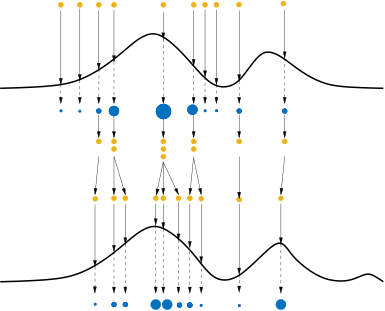
\includegraphics[width=0.88\textwidth]{Figures/particle_filter}} at (0, 0);
    
    \node [] (a) at (-0.5, 4.6) {$N$ particles};
    
    \node [align=left, right] (a) at (-5.7, 1.1) {Weight};
    \node [align=left, right] (a) at (-5.7, 0.2) {Resample};
    \node [align=left, right] (a) at (-5.7, -1.1) {Propagate \\ particles};
    \node [align=left, right] (a) at (-5.7, -4.1) {Weight};
    
    \node [align=left, right] (a) at (2.6, 4.15) {$\Big\{\big(\hat{\bm{x}}^{(i)}_{k-1}, N^{-1}\big)\Big\}_{i=1}^N$};
    \node [align=left, right] (a) at (2.6, 3) {Likelihood \\ function $p(\bm{z}_k\,|\,\bm{x}_k)$};
    \node [align=left, right] (a) at (2.6, 1.25) {$\Big\{\big(\hat{\bm{x}}^{(i)}_{k-1}, \tilde{w}^{(i)}_{k-1}\big)\Big\}_{i=1}^N$};
    \node [align=left, right] (a) at (2.6, 0.2) {$\Big\{\big(\bm{x}^{(i)}_{k-1}, N^{-1}\big)\Big\}_{i=1}^N$};
    \node [align=left, right] (a) at (2.6, -1.1) {$\Big\{\big(\hat{\bm{x}}^{(i)}_{k}, N^{-1}\big)\Big\}_{i=1}^N$};
    \node [align=left, right] (a) at (2.6, -4) {$\Big\{\big(\hat{\bm{x}}^{(i)}_{k}, \tilde{w}^{(i)}_{k}\big)\Big\}_{i=1}^N$};
    
\end{tikzpicture}
\caption[Evolution of the empirical probability distributions estimated by the bootstrap filter.]{Evolution of the empirical probability distributions estimated by the bootstrap filter. The filter starts at time $k-1$ with the unweighted particles $\big\{\big(\hat{\bm{x}}^{(i)}_{k-1}, N^{-1}\big)\big\}_{i=1}^N$, which provide an approximation of $p(\bm{x}_{k-1}\,|\,\bm{x}^{(i)}_{k-2}, \bm{u}_{k-2})$. Computing the importance weights yields an approximation of $p(\bm{x}_{k-1}\,|\,\bm{Y}_{k-1}, \bm{U}_{k-1})$ given by the set $\big\{\big(\hat{\bm{x}}^{(i)}_{k-1}, \tilde{w}^{(i)}_{k-1}\big)\big\}_{i=1}^N$. In the resampling step, the fittest particles are reproduced to obtain $\big\{\big(\bm{x}^{(i)}_{k-1}, N^{-1}\big)\big\}_{i=1}^N$, which again approximates $p(\bm{x}_{k-1}\,|\,\bm{Y}_{k-1}, \bm{U}_{k-1})$. Finally, closing the filter loop, the prediction step produces variety, resulting in $\big\{\big(\hat{\bm{x}}^{(i)}_{k}, N^{-1}\big)\big\}_{i=1}^N$, an approximation of $p(\bm{x}_{k}\,|\,\bm{x}^{(i)}_{k-1}, \bm{u}_{k-1})$ \cite{merwe2000scented}.}
	\label{fig:bootstrap}
\end{figure}

%\begin{figure}[t]
%\centering
%\begin{tikzpicture}[scale=1.0, auto, thick, node distance=3cm,>=latex']
%    \pgftext{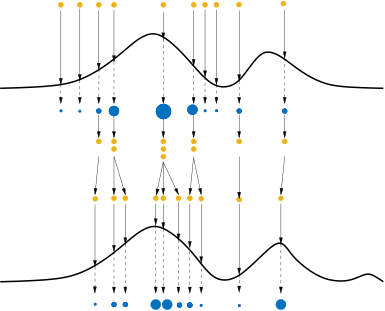
\includegraphics[width=0.88\textwidth]{Figures/particle_filter}} at (0, 0);
%    
%    \node [] (a) at (-0.5, 4.6) {$N$ particles};
%    
%    \node [align=left, right] (a) at (-5.7, 1.1) {Weight};
%    \node [align=left, right] (a) at (-5.7, 0.2) {Resample};
%    \node [align=left, right] (a) at (-5.7, -1.1) {Draw particles \\ from proposal \\ distribution};
%    \node [align=left, right] (a) at (-5.7, -4.1) {Weight};
%    
%    \node [align=left, right] (a) at (2.6, 4.15) {$p(\bm{x}_{k-1}\,|\,\bm{x}_{k-2}, \bm{u}_{k-2})$};
%    \node [align=left, right] (a) at (2.6, 3) {Likelihood \\ function $p(\bm{z}_k\,|\,\bm{x}_k)$};
%    \node [align=left, right] (a) at (2.6, 1.25) {$p(\bm{x}_{k-1}\,|\,\bm{Y}_{k-1}, \bm{U}_{k-2})$};
%    \node [align=left, right] (a) at (2.6, 0.2) {$p(\bm{x}_{k-1}\,|\,\bm{Y}_{k-1}, \bm{U}_{k-2})$};
%    \node [align=left, right] (a) at (2.6, -1.1) {$p(\bm{x}_{k}\,|\,\bm{x}_{k-1}, \bm{u}_{k-1})$};
%    \node [align=left, right] (a) at (2.6, -4) {$p(\bm{x}_{k}\,|\,\bm{Y}_{k}, \bm{U}_{k-1})$};
%    
%\end{tikzpicture}
%\caption{Bootstrap filter starting at time $k-1$ with the unweighted particles $\Big\{\big(\hat{\bm{x}}^{(i)}_{k-1}, N^{-1}\big)\Big\}_{i=1}^N$, which provide an approximation of $p(\bm{x}_{k-1}\,|\,\bm{x}_{k-2}, \bm{u}_{k-2})$. Computing the importance weights results in $\Big\{\big(\hat{\bm{x}}^{(i)}_{k-1}, \tilde{w}^{(i)}_{k-1}\big)\Big\}_{i=1}^N$ yielding an approximation of $p(\bm{x}_{k-1}\,|\,\bm{Y}_{k-1}, \bm{U}_{k-2})$. Subsequently, in the resampling step the fittest particles are reproduced to obtain $\Big\{\big(\bm{x}^{(i)}_{k-1}, N^{-1}\big)\Big\}_{i=1}^N$, which again approximates $p(\bm{x}_{k-1}\,|\,\bm{Y}_{k-1}, \bm{U}_{k-2})$. Finally, the prediction step produces variety, resulting in $\Big\{\big(\hat{\bm{x}}^{(i)}_{k}, N^{-1}\big)\Big\}_{i=1}^N$, which approximates $p(\bm{x}_{k}\,|\,\bm{x}_{k-1}, \bm{u}_{k-1})$  \cite{merwe2000scented}.}
%	\label{fig:resampling_distributions}
%\end{figure}




\subsection{The Unscented Particle Filter}\label{sec:unscented_particle}

\noindent
\citeauthor{daum2005nonlinear} pointed out in \cite{daum2005nonlinear} that in most of the successful implementations of particle filters the proposal distribution is obtained using an extended Kalman filter or an unscented Kalman filter. Both filters compute recursive Gaussian approximations of the posterior filtering distribution,

\begin{equation}
  p\big(\bm{x}_k\,|\,\bm{Z}_{k}, \bm{U}_{k-1}\big) \approx p_{\mathcal{N}}\big(\bm{x}_k\,|\,\bm{Z}_{k}, \bm{U}_{k-1}\big) = \mathcal{N}\big(\hat{\bm{x}}_{k},\bm{P}_k\big)\,.
\end{equation}

\noindent
 incorporating the latest measurement at each time step. Within the particle filter framework, the EKF or UKF can be used to propagate a Gaussian proposal distribution for each particle, 

\begin{equation}
  \pi\big(\bm{x}_{k}\,|\,\bm{X}^{(i)}_{k-1}, \bm{Z}_{k}, \bm{U}_{k-1}\big) = \mathcal{N}\big(\bar{\bm{x}}^{(i)}_k,\bm{P}^{(i)}_k\big), \quad i \in \{1, \dots, N\}\,.
\end{equation}

\noindent
The $i$-th particle at time step $k$ is then sampled from this distribution,

\begin{equation}\label{eq:sample_proposal}
  \hat{\bm{x}}^{(i)}_k \sim \pi\big(\bm{x}_k\,|\,\bm{X}^{(i)}_{k-1}, \bm{Z}_{k}, \bm{U}_{k-1}\big), \quad k > 0,  \quad i \in \{1, \dots, N\}\,.
\end{equation}


Although the individual proposal distributions for each particle are Gaussian, in general, the form of the overall proposal distribution $\pi(\bm{x}_{k}\,|\,\bm{X}_{k-1}, \bm{Z}_{k}, \bm{U}_{k-1})$ will not be Gaussian. Though, the peak of the proposal distribution is moved towards the peak of the likelihood function, therefore moving particles to regions of high likelihood, as illustrated in Figure \ref{fig:proposal_distribution}. Scenario (a) depicts little overlap of the proposal distribution and the likelihood function, which may be the case when the available model is not sufficiently accurate. Scenario (b) depicts peaked likelihood, which represents very accurate measurements.

\begin{figure}[t]
\centering
\begin{subfigure}[]
   \centering
\begin{tikzpicture}[scale=1.0, auto, thick, node distance=3cm,>=latex']
    \pgftext{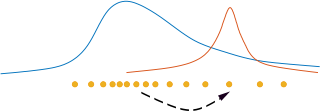
\includegraphics[width=0.88\textwidth]{Figures/little_overlap}} at (0, 0);
    
    \node [align=left, right] (a) at (-5, 1) {Proposal \\ distribution};
    \node [align=left, right] (a) at (3, 1) {Likelihood \\ function};
    \node [align=left, right] (a) at (-3, -1.5) {Particles};
\end{tikzpicture}
\end{subfigure}

\begin{subfigure}[]
   \centering
\begin{tikzpicture}[scale=1.0, auto, thick, node distance=3cm,>=latex']
    \pgftext{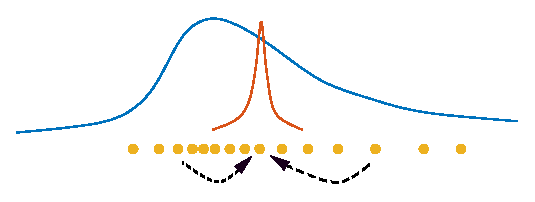
\includegraphics[width=0.88\textwidth]{Figures/peaked_likelihood}} at (0, 0);
\end{tikzpicture}
\end{subfigure}

\caption[The two scenarios in which a parametric filter such as the EKF or UKF may help generating better proposal distributions by moving particles to regions of high likelihood.]{The two scenarios in which a parametric filter such as the EKF or UKF may help generating better proposal distributions by moving particles to regions of high likelihood: (a) when there is little overlap of proposal distribution and likelihood function, that is when the peak of the likelihood happens to lie in one of the tails of the proposal distribution or (b) when the likelihood function is very narrow, which is the case for very accurate measurements.}
\label{fig:proposal_distribution}
\end{figure}



\citeauthor{van2001unscented} \cite{van2001unscented} proposed to use an unscented Kalman filter in order to incorporate the latest measurement and thus to generate better proposal distributions. Based on the ability of the UKF to more accurately propagate the mean and covariance of the state distribution, when compared to the EKF, the result is a bigger support overlap with the true posterior distribution. The resulting filter is referred to as the \emph{unscented particle filter}.


Figure \ref{fig:unscented_particle_filter_cycle} depicts the entire unscented particle filter algorithm, including the calculation of sigma points for each particle, the time and measurement update step, as well as the importance sampling and resampling step. Note that we denote the mean of the Gaussian proposal distribution of the $i$-th particle with $\bar{\bm{x}}^{(i)}_k$, being consistent with former notation of the mean. For the $i$-th hypothesis $\hat{\bm{x}}^{(i)}$ of the state we continue to use a hat.

\tikzstyle{block} = [draw, rectangle, thick, 
    minimum height=1.5cm, minimum width=10.9cm]
\tikzstyle{output} = [coordinate]

\begin{figure}
\centering
\begin{tikzpicture}[auto, rounded corners=1pt, node distance=5cm,>=latex']
    
\node [block, align=center] (init) {\emph{Initialisation} \\[3mm] 
	Draw $N$ samples $\bm{x}^{(i)}_0$ from the initial state distribution: \\[2mm]
	$\Big\{\big(\bm{x}^{(i)}_{0}, N^{-1}\big)\Big\}_{i=1}^N, \quad \bm{x}^{(i)}_0 \sim p(\bm{x}_0)\,,$ \\[2mm]
	$\bar{\bm{x}}_0^{(i)} = \mathbb{E}\Big[\bm{x}_0^{(i)}\Big], \quad \bar{\bm{x}}^{(i)a}_0 = \bigg[\bar{\bm{x}}_0^{(i)T}, \mathbb{E}\Big[{\bm{w}_0}^T\Big], \mathbb{E}\Big[{\bm{v}_{0}}^T\Big] \bigg]^T\,,$ \\[2mm]
	$\bm{P}^{(i)}_{0} = \mathbb{E}\Big[\big(\bm{x}^{(i)}_{0} - \bar{\bm{x}}^{(i)}_{0}\big) \big(\bm{x}^{(i)}_{0} - \bar{\bm{x}}^{(i)}_{0}\big)^T\Big]\,,$ \\[2mm]
	$\bm{P}^{(i)a}_{0} = \mathbb{E}\Big[\big(\bm{x}^{(i)a}_{0} - \bar{\bm{x}}^{(i)a}_{0}\big) \big(\bm{x}^{(i)a}_{0} - \bar{\bm{x}}^{(i)a}_{0}\big)^T\Big] = \begin{bsmallmatrix}
  \bm{P}^{(i)}_0 & \bm{0} & \bm{0} \\
  \bm{0} & \bm{Q}_0 & \bm{0} \\
  \bm{0} & \bm{0} & \bm{R}_0 \\
\end{bsmallmatrix}$};
\node [block, align=center, below of=init, node distance=4.9cm] (sigma) {\emph{Calculation of sigma points} \\[3mm] 
	$\bm{\mathcal{X}}^{(i)a}_{k-1} = \Big\{\bar{\bm{x}}^{(i)a}_{k-1}, \quad \bar{\bm{x}}^{(i)a}_{k-1} + \gamma_a \sqrt{\bm{P}^{(i)a}_{k-1}}, \quad \bar{\bm{x}}^{(i)a}_{k-1} - \gamma_a \sqrt{\bm{P}^{(i)a}_{k-1}}\Big\}$};
\node [block, align=center, below of=sigma, node distance=4.7cm] (predict) {\emph{Time update} \\[3mm] 
	Propagate sigma points: \\ 
	$\bm{\mathcal{X}}^{(i)\bm{x}}_{k|k-1} = \bm{\phi}_{k-1}\big(\bm{\mathcal{X}}^{(i)\bm{x}}_{k-1}, \bm{u}_{k-1}, \bm{\mathcal{X}}^{(i)\bm{w}}_{k-1}\big)$ \\[2mm]
	Compute a priori state estimate: \\ 
	$\bar{\bm{x}}^{(i)}_{k|k-1} = \sum^{2l}_{j = 0} W_j^{(m)} \mathcal{X}^{(i)\bm{x}}_{j, k\,|\,k-1}$ \\[2mm]
	Compute a priori error covariance: \\ 
	$\bm{P}^{(i)}_{k|k-1} = \sum^{2l}_{j = 0} W_j^{(c)} \big(\mathcal{X}^{(i)\bm{x}}_{j, k\,|\,k-1} -\bar{\bm{x}}^{(i)}_{k|k-1}\big)\big(\mathcal{X}^{(i)\bm{x}}_{j, k\,|\,k-1}-\bar{\bm{x}}^{(i)}_{k|k-1}\big)^T$ \\[2mm]
	Predict measurement: \\ 
	$\bm{\mathcal{Z}}^{(i)}_{k|k-1} = \bm{h}_{k}\big(\bm{\mathcal{X}}^{(i)\bm{x}}_{k|k-1}, \bm{\mathcal{X}}^{(i)\bm{v}}_{k|k-1}\big)$ \\[1mm]
	$\bar{\bm{z}}^{(i)}_{k|k-1} = \sum^{2l}_{j = 0} W_j^{(m)} \mathcal{Z}^{(i)}_{j, k\,|\,k-1}$};
\node [block, align=center, below of=predict, node distance=7.3cm] (update) {\emph{Measurement update} \\[3mm] 
	Compute innovation and cross covariance matrices: \\ 
	$\bm{P}^{(i)}_{\tilde{\bm{z}}_k \tilde{\bm{z}}_k} = \sum^{2l}_{j = 0} W_j^{(c)} \big(\mathcal{Z}^{(i)}_{j, k\,|\,k-1} -\bar{\bm{z}}^{(i)}_{k|k-1}\big)\big(\mathcal{Z}^{(i)}_{j, k\,|\,k-1}-\bar{\bm{z}}^{(i)}_{k|k-1}\big)^T$ \\[2mm]
	$\bm{P}^{(i)}_{\tilde{\bm{x}}_k \tilde{\bm{z}}_k} = \sum^{2l}_{j = 0} W_j^{(c)} \big(\mathcal{X}^{(i)\bm{x}}_{j, k\,|\,k-1} -\bar{\bm{x}}^{(i)}_{k|k-1}\big)\big(\mathcal{Z}^{(i)}_{j, k\,|\,k-1}-\bar{\bm{z}}^{(i)}_{k|k-1}\big)^T$ \\[2mm]
	Compute Kalman gain: \\
	$\mathcal{K}^{(i)}_k = \bm{P}^{(i)}_{\tilde{\bm{x}}_k \tilde{\bm{z}}_k}{\bm{P}^{(i)}_{\bm{z}_k\bm{z}_k}}^{-1}$ \\[2mm]
	Compute a posteriori mean: \\ $ \bar{\bm{x}}^{(i)}_k = \bar{\bm{x}}^{(i)}_{k|k-1} + \mathcal{K}^{(i)}_k\big(\bm{z}_k - \bar{\bm{z}}^{(i)}_{k|k-1}\big)$ \\[2mm]
	Update error covariance: \\ $\bm{P}^{(i)}_k = \bm{P}^{(i)}_{k|k-1} - \mathcal{K}^{(i)}_k \bm{P}^{(i)}_{\tilde{\bm{z}}_k \tilde{\bm{z}}_k} {\mathcal{K}^{(i)}_k}^T$};

\node [output, below of=update, node distance=4.2cm, name=output] {};
\node [output, right of=output, node distance=5.9cm, name=help2] {};
\node [output, below of=init, node distance=3.5cm, name=help4] {};
\node [output, right of=help4, node distance=5.9cm, name=help3] {};

\draw [draw,-stealth, thick, align=left] (init) -- (sigma);
\draw [draw,-stealth, thick, align=left] (sigma) -- (predict);
\draw [draw,-stealth, thick, align=left] (predict) -- (update);
\draw [draw,-stealth, thick, align=left] (update) -- node [label={left:$\vdots$}, name=dots]{} (output);
\node [right of=dots, node distance=5.6cm] {$\vdots$};
\draw [draw,-stealth, thick] (help2) -- (help3) -- (help4);
\end{tikzpicture}
\end{figure}



\tikzstyle{block} = [draw, rectangle, thick, 
    minimum height=1.5cm, minimum width=11cm]
\tikzstyle{output} = [coordinate]

\begin{figure}
\centering
\begin{tikzpicture}[auto, rounded corners=1pt, node distance=5cm,>=latex']
    
\node [] (init) {$\vdots$};
\node [block, align=center, below of=init, node distance=4.3cm] (predict) {\emph{Importance sampling step} \\[3mm] 
	Draw $N$ samples $\hat{\bm{x}}^{(i)}_k$ from the proposal distribution: \\
	$\Big\{\big(\hat{\bm{x}}^{(i)}_{k}, N^{-1}\big)\Big\}_{i=1}^N,$  \\[2mm]
	$\hat{\bm{x}}^{(i)}_k \sim \pi\big(\bm{x}_k\,|\,\bm{X}^{(i)}_{k-1}, \bm{Z}_{k}, \bm{U}_{k-1}\big) = \mathcal{N}(\bar{\bm{x}}^{(i)}_{k},\bm{P}^{(i)}_k)$ \\[2mm]
	Evaluate importance weights: \\
	$w^{(i)}_k = w^{(i)}_{k-1} \frac{p\big(\bm{z}_k\,|\,\hat{\bm{x}}^{(i)}_k\big) p\big(\hat{\bm{x}}^{(i)}_k\,|\,\bm{x}^{(i)}_{k-1}, \bm{u}_{k-1}\big)}{\pi\big(\hat{\bm{x}}^{(i)}_k\,|\,\bm{X}^{(i)}_{k-1}, \bm{Z}_{k}, \bm{U}_{k-1}\big)}, \quad i \in \{1, \dots, N\}$ \\[2mm]
	Normalise importance weights: \\
	$\tilde{w}^{(i)}_k = w^{(i)}_{k} \Big[\sum^N_{j = 1} w^{(j)}_k\Big]^{-1}, \quad i \in \{1, \dots, N\}$};
	\node [block, align=center, below of=predict, node distance=5cm] (update) {\emph{Resampling step} \\[3mm] 
	Draw $N$ samples $\bm{x}^{(i)}_{k}$ from the set $\Big\{\big(\hat{\bm{x}}^{(j)}_{k}, \tilde{w}^{(j)}_{k}\big)\Big\}_{j=1}^N$: \\[1mm]
	$\Big\{\big(\bm{x}^{(i)}_{k}, N^{-1}\big)\Big\}_{i=1}^N, \quad \operatorname{Pr}\big(\bm{x}^{(i)}_k = \hat{\bm{x}}^{(j)}_k\big) = \tilde{w}^{(j)}_k, \quad j \in \{1, \dots, N\}$};
	\node [block, align=center, below of=update, node distance=3.5cm] (outputblock) {\emph{Recombine particles} \\[3mm] 
	Compute conditional mean: \\
	$\hat{\bm{x}}_k = \tilde{\mathbb{E}}_{p(\bm{x}_k\,|\,\bm{Z}_{k}, \bm{U}_{k-1})}\big[\bm{x}_k\big] = \frac{1}{N} \sum^N_{i = 1} \bm{x}^{(i)}_k$ \\[2mm]
	Compute covariance: \\
	$\bm{P}_k = \sum^N_{i = 1} \big(\bm{x}^{(i)}_k - \hat{\bm{x}}_{k}\big) \big(\bm{x}^{(i)}_k - \hat{\bm{x}}_{k}\big)^T$};

\node [output, below of=outputblock, node distance=2.8cm, name=output] {Output};
\node [output, below of=outputblock, node distance=2.2cm, name=help1] {};
\node [output, right of=help1, node distance=6.1cm, name=help2] {};
\node [above of=help2, node distance=15cm, name=help3] {$\vdots$};

\draw [draw,-stealth, thick, align=left] (init) -- (predict);
\draw [draw,-stealth, thick, align=left] (predict) -- (update);
\draw [draw,-stealth, thick, align=left] (update) -- (outputblock);
\draw [draw,-stealth, thick, align=left] (outputblock) -- node [label={left:Output}]{} (output);
\draw [draw,-stealth, thick] (help1) -- (help2) -- (help3);
\end{tikzpicture}
\caption[Operation cycle of the unscented particle filter.]{Operation cycle of the unscented particle filter, illustrating the calculation of sigma points for each particle, the time and measurement update step, as well as the importance sampling and resampling step. Finally, the particles are recombined to obtain the minimum mean-squared error estimate and the corresponding covariance.} \label{fig:unscented_particle_filter_cycle}
\end{figure}



\section{Interval Analysis}

Built on the foundation of set theory, \emph{interval analysis} encompasses numerical methods that yield reliable results. Originating back to Moore's doctorate on the use of intervals to analyse and control numerical errors in digital computers in 1962, interval computation has come a long way and has been subject to extensive research since.  As opposed to the probabilistic methods presented above, which provide a point estimate associated with a given uncertainty in the form of a probability distribution, interval computations provide a box guaranteed to contain the solution, given that the problem is well modelled and the assumptions are sufficiently conservative. However, this guarantee comes with the trade-off that any point in the confined solution space is assumed to be equally likely. 


As we shall see below, self-localisation can be modelled as an optimisation problem. In \cite{Rokne2001}, \citeauthor{Rokne2001} states the following advantages of interval methods to global optimisation problems. They

\begin{itemize}
	\item do not rely on starting points,
	\item can prove existence, absence, and uniqueness of solutions,
	\item can easily accommodate external constraints,
	\item and are reliable in that they never discard a feasible solution.
\end{itemize}

\noindent
An in-depth presentation of the following basic concepts can be found in \cite{jaulin2001applied}.


\subsection{Basic Concepts}
\label{sec: interval_basic_concepts}

Let $[x]$ denote a \emph{closed interval}, defined as a closed subset of the real numbers given by

\begin{equation}
  [x] = \big[\underline{x}, \overline{x}\big] = \big\{x \in \mathbb{R} \,\,|\,\, \underline{x} \leq x \leq \overline{x}\big\}\,,
\end{equation}

\noindent
 where $\underline{x}$ and $\overline{x}$ are called the \emph{lower bound} and the \emph{upper bound} of the interval, respectively. An interval $[x]$ can be assigned a \emph{width} $\operatorname{w}\big([x]\big)$, a \emph{midpoint} $\operatorname{mid}\big([x]\big)$, and an \emph{absolute value} $\big|[x]\big|$, given by

\begin{align}
\operatorname{w}\big([x]\big) &= \overline{x} - \underline{x}\,, \\
\operatorname{mid}\big([x]\big) &= \frac{\underline{x} + \overline{x}}{2}\,, \\
\big|[x]\big| &= \max\big(|\underline{x}|, |\overline{x}|\big) \,,
\end{align}


\noindent
respectively. We denote the set of closed intervals with endpoints in the set of real numbers augmented by plus and minus infinity with
 
 \begin{equation}
 [\mathbb{R}] = \Big\{\big[\underline{x}, \overline{x}\big] \,|\: \underline{x}, \overline{x} \in \mathbb{R} \cup \{-\infty, \infty\}, \quad \underline{x} \leq \overline{x}\Big\} \cup \emptyset \,.
 \end{equation} 
 
 \noindent
Note that we include the empty set, in order to form a closed interval system, that is, a system in which there are no undefined operator-operand or function-argument combinations \cite{hansen2003global}.

The \emph{intersection} of two intervals $[x]$ and $[y] \in [\mathbb{R}]$ is defined as the interval

 \begin{equation}
 \begin{split}
  [x] \cap [y] &= \big\{ z \in \mathbb{R}\,\,|\,\, z \in [x] \:\mbox{and}\: z \in [y] \big\} \\
  &= \begin{cases}
  	\big[\max(\underline{x}, \underline{y}), \min(\overline{x}, \overline{y})\big] & \quad \mathrm{if}\:\max(\underline{x}, \underline{y}) \leq \min(\overline{x}, \overline{y}) \\
  	\emptyset & \quad \mathrm{otherwise}
  \end{cases}\,.
\end{split}
\end{equation}

\noindent
While the intersection is always an interval, this is not true for the \emph{union} of $[x]$ and $[y]$, given by

 \begin{equation}
  [x] \cup [y] = \big\{ z \in \mathbb{R}\,\,|\,\, z \in [x] \:\mbox{or}\: z \in [y] \big\} \,.
  \end{equation}

\noindent
To make the set of intervals closed with respect to the union, we define the \emph{interval hull} of a subset $\mathbb{X} \in \mathbb{R}$ as the smallest interval $[\mathbb{X}]$ that contains it. Now, we can define the \emph{interval union} of $[x]$ and $[y]$ as the interval hull of the union $[x] \cup [y]$,

 \begin{equation}
  \begin{split}
  [x] \sqcup [y] &= \big[[x] \cup [y]\big] \\
  &= \big[\min(\underline{x}, \underline{y}), \max(\overline{x}, \overline{y})\big]\,.
  \end{split}
  \end{equation}

Multiplication of a real number $\alpha$ with an interval $[x]$ is defined as

 \begin{equation}
 \begin{split}
  \alpha[x] &= \big\{ \alpha x \,\,|\,\, x \in [x]\big\} \\
  &= \begin{cases}
  	\big[\alpha\underline{x}, \alpha\overline{x}\big] & \quad \mathrm{if}\:\alpha \geq 0 \\
  	\big[\alpha\overline{x}, \alpha\underline{x}\big] & \quad \mathrm{if}\:\alpha < 0
  \end{cases}\,.
\end{split}
\end{equation}

\noindent
An inner binary operation $\circ$ on the real intervals $[x], [y] \in [\mathbb{R}]$ is defined by
 
 \begin{equation}
  [x] {\,\circ\,} [y] = \big\{ x {\,\circ\,} y \in \mathbb{R}\,\,|\,\, x \in [x] \,\mbox{and}\, y \in [y] \big\}\,.
\end{equation}

\noindent
Hence, the four basic arithmetic operations on intervals are given by

\begin{align}
	[x] + [y] &= \Big[\underline{x} + \underline{y}, \overline{x} + \overline{y}\Big] \\
	[x] - [y] &= \Big[\underline{x} - \overline{y}, \overline{x} - \underline{y}\Big]\\
	\begin{split}
[x] \cdot [y] &= \Big[ \min\big(\underline{x} {\cdot} \underline{y}, \underline{x} \cdot \overline{y}, \overline{x} \cdot \underline{y}, \overline{x} \cdot \overline{y}\big), \\
&\mathrel{\phantom{=[}}\max\big(\underline{x} \cdot \underline{y}, \underline{x} \cdot \overline{y}, \overline{x} \cdot \underline{y}, \overline{x} \cdot \overline{y}\big) \Big]
\end{split} \\
\begin{split}
\frac{[x]}{[y]} &= \bigg[ \min\Big(\frac{\underline{x}}{\underline{y}}, \frac{\underline{x}}{\overline{y}}, \frac{\overline{x}}{\underline{y}}, \frac{\overline{x}}{\overline{y}}\Big), \\
&\mathrel{\phantom{=[}}\max\Big(\frac{\underline{x}}{\underline{y}}, \frac{\underline{x}}{\overline{y}}, \frac{\overline{x}}{\underline{y}}, \frac{\overline{x}}{\overline{y}}\Big) \bigg], \quad 0 \notin [y]
\end{split}
\end{align}

\noindent
These definitions are motivated by the following argument: Given two intervals $[x]$ and $[y]$ and two exact values $x \in [x]$ and $y \in [y]$, it is guaranteed that $x \circ y \in \big([x] \circ [y]\big)$, even though the exact values of $x$ and $y$ may not be known \cite{Rokne2001}.

\begin{figure}[t]
\centering
\begin{tikzpicture}[scale=1.0, auto, thick, node distance=3cm,>=latex']
    \pgftext{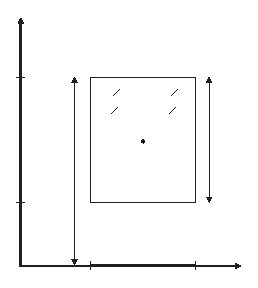
\includegraphics[width=0.50\textwidth]{Figures/interval}} at (0, 0);
    
    \node [] (a) at (0.36, 1) {$[\bm{x}]$};
    \node [] (a) at (0.36, -3.6) {$[x_1]$};
     \node [] (a) at (0.36, -0.4) {$\operatorname{mid}\big([\bm{x}]\big)$};
    \node [] (a) at (-3.4, 0.1) {$[x_2]$};
    \node [] (a) at (-2, 0.1) {$\big|\big|[\bm{x}]\big|\big|$};
    \node [] (a) at (2.8, 0.1) {$\operatorname{w}\big([\bm{x}]\big)$};
        
\end{tikzpicture}
\caption[The projection of an interval vector onto its axes, its width, norm, and midpoint.]{The projection of an interval vector $[\bm{x}] = \big[[x_1], [x_2]\big] \in [\mathbb{R}]^2$ onto the two axes as well as its width $\operatorname{w}\big([\bm{x}]\big)$, norm $\big|\big|[\bm{x}]\big|\big|$, and midpoint $\operatorname{mid}\big([\bm{x}]\big)$, \cite{moore2009introduction}.}
	\label{fig:interval_analysis}
\end{figure}
 
A \emph{real interval vector} $[\bm{x}] = \big([x_1], [x_2], \dots, [x_n]\big)^T \in [\mathbb{R}]^n$, also called a \emph{box}, is defined as the Cartesian product of $n$ real intervals, 
 
 \begin{equation}
  [\bm{x}] = [x_1] \times [x_2] \times \dots \times [x_n]\,,
\end{equation}

\noindent
where the $i$-th interval component $[x_i]$ represents the projection of $[\bm{x}]$ onto the $i$-th axis. We define multiplication of an interval vector with a real number and the addition and multiplication of two interval vectors as follows:

\begin{align}
\alpha[\bm{x}] &= \big(\alpha [x_1], \dots, \alpha [x_n]\big)\,, \\
[\bm{x}] + [\bm{y}] &= \big([x_1] + [y_1], \dots, [x_n] + [y_n]\big)\,, \\
[\bm{x}]^T \cdot [\bm{y}] &= [x_1] \cdot [y_1] + \cdots + [x_n] \cdot [y_n] \,.
\end{align}

\noindent
Likewise, the width and the midpoint can be extended naturally to interval vectors as follows:


\begin{align}
\operatorname{w}\big([\bm{x}]\big) &= \underset{1 \leq i \leq n}{\max}\Big(\operatorname{w}\big([x_i]\big)\Big) \\
\operatorname{mid}\big([\bm{x}]\big) &= \bigg[\operatorname{mid}\big([x_1]\big), \dots , \operatorname{mid}\big[x_n]\big)\bigg]^T\,.
\end{align}

\noindent
A box can be assigned a norm $\big|\big|[\bm{x}]\big|\big|$, which represents a generalisation of the absolute value, given by

\begin{equation}
\big|\big|[\bm{x}]\big|\big| = \underset{1 \leq i \leq n}{\max}\Big(\big|[x_i]\big|\Big)\,.
\end{equation}



\noindent
The projection of an interval vector $[\bm{x}]$ onto the $i$-th axis as well as its width, norm, and midpoint is depicted in Figure \ref{fig:interval_analysis} for $n = 2$.



Let $\bm{f}: \mathbb{R}^n \rightarrow \mathbb{R}^m$, $[\bm{x}] \in [\mathbb{R}]^n$, and $\bm{f}\big([\bm{x}]\big)$ the image of $[\bm{x}]$ under $\bm{f}$, given by

\begin{equation}
\bm{f}\big([\bm{x}]\big) = \big\{f(\bm{x}) \,|\, \bm{x} \in [\bm{x}]\big\} \,.
\end{equation}

\noindent
An interval function $[\bm{f}]: [\mathbb{R}]^n \rightarrow [\mathbb{R}]^m$ is called \emph{inclusion function} of $\bm{f}$ if
 
 \begin{equation}
  \bm{f}\big([\bm{x}]\big) \subseteq [\bm{f}]\big([\bm{x}]\big), \quad \forall [\bm{x}] \in [\mathbb{R}]^n\,.
\end{equation}

\noindent
The simplest way of obtaining an inclusion function $[\bm{f}]$ of a given function $\bm{f}$ is to replace each real variable by their \emph{natural interval extension}. The resulting function is called the \emph{natural inclusion function}. If $[\bm{f}]$ is the inclusion function that determines the smallest possible box comprising $\bm{f}\big([\bm{x}]\big)$ it is called \emph{minimal} and denoted by $[\bm{f}]^{\ast} \big([\bm{x}]\big)$. Figure \ref{fig:inclusion_functions} depicts the image of a box $[\bm{x}]$ under $\bm{f}$ and two of its possible inclusion functions, one of them the minimal inclusion function $[\bm{f}]^{*}\big([\bm{x}]\big)$.

Since the minimal inclusion function is usually not available a so-called contractor can be used to minimise a known inclusion function instead. Before we elaborate on contractors in Section \ref{sec:contractors}, we will introduce a generic description of problems involving constraints in the next section.


\begin{figure}[t]
\centering
\begin{tikzpicture}[scale=1.0, auto, thick, node distance=3cm,>=latex']
    \pgftext{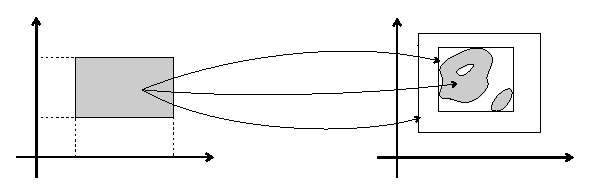
\includegraphics[width=0.98\textwidth]{Figures/inclusion}} at (0, 0);
    
    \node [] (a) at (0.36, 1.3) {$[\bm{f}]^{*}([\bm{x}])$};
     \node [] (a) at (0.36, 0.4) {$\bm{f}([\bm{x}])$};
     \node [] (a) at (0.36, -0.33) {$[\bm{f}]([\bm{x}])$};
    \node [] (a) at (-3.6, 0.15) {$[\bm{x}]$};
    
    \node [align=center] (a) at (-1.9, -1.52) {$x_1$};
    \node [align=center] (a) at (-2.4, -1.5) {$\overline{x}_1$};
    \node [align=center] (a) at (-4.5, -1.5) {$\underline{x}_1$};
    
    \node [] (a) at (5.5, -1.5) {$y_1$};
    
    \node [] (a) at (-5.8, 1.3) {$x_2$};
    \node [] (a) at (1.6, 1.3) {$y_2$};
    \node [] (a) at (-5.8, 0.8) {$\overline{x}_2$};
    \node [] (a) at (-5.8, -0.35) {$\underline{x}_2$};
        
\end{tikzpicture}
\caption[Image of an interval box and two inclusion functions.]{Image $\bm{f}\big([\bm{x}]\big)$ of a box $[\bm{x}] \in [\mathbb{R}]^2$ under $\bm{f}: \mathbb{R}^2 \rightarrow \mathbb{R}^2$ and two inclusion functions $[\bm{f}]\big([\bm{x}]\big)$ and $[\bm{f}]^{*}\big([\bm{x}]\big)$. The interval function $[\bm{f}]^{*}$ is the minimal inclusion function \cite{jaulin2001applied}.}
	\label{fig:inclusion_functions}
\end{figure}


\subsection{Constraint Satisfaction Problems}\label{sec:csp}

Utilising the notion of constraints is a formal and declarative way of describing certain problems, abstracting from a domain-specific description in order to allow the solution of the problem with efficient, generic solution methods. Formally, a \emph{constraint satisfaction problem} (CSP) is defined as a triple $(\mathbb{X}, \mathbb{D}, \mathbb{C})$, where $\mathbb{X} = \{x_{1}, \dots ,x_{n}\}$ is a finite set of variables with their associated non-empty domains $\mathbb{D} = \{D_{1}, \dots ,D_{n}\}$, so that $x_i \in D_i$, and $\mathbb{C} = \{C_{1}, \dots ,C_{m}\}$ is a finite set of constraints. Each of the constraints $C_j \in \mathbb{C}$ in turn is a pair $(\mathbb{T}_j, R_j)$, where $\mathbb{T}_j = \{x_{j,1}, \dots, x_{j,k}\} \subseteq \mathbb{X}$ is a subset of the variables and $R_j$ is a $k$-ary relation on the corresponding subset of domains $\mathbb{D}_j = \{D_{j1}, \dots, D_{jk}\} \subseteq \mathbb{D}$, reducing possible combinations of the values of variables to a subset of $D_{j1} \times \dots \times D_{jk}$.

If the domains $D_{i}$ are real intervals $[x_i]$ and the constraints have the form of equalities or inequalities, so that the relation $R_j$ is either of the form

\begin{equation}\label{eq:individual_constraints}
  f_j(x_{1}, \dots ,x_{k}) = 0, \quad j \in \{1, \dots ,m\}\,,
\end{equation}

\noindent
or of the form

\begin{equation}
  f_j(x_{1}, \dots ,x_{k}) \leq 0, \quad j \in \{1, \dots ,m\}\,,
\end{equation}

\noindent
we call this a \emph{numerical constraint satisfaction problem} (NCSP). In the latter case we can introduce a slack variable $x_{sj} \geq 0$ to cast the inequality constraint to an equality constraint as follows:

\begin{equation}
  f_j(x_{1}, \dots ,x_{k}) + x_{sj} = 0, \quad j \in \{1, \dots ,m\}\,.
\end{equation}

Now, we combine the $n$ scalar variables to form a real vector $\bm{x} = (x_{1}, \dots ,x_{n})^T \in \mathbb{R}^n$ with its domain $[\bm{x}_0] = \big([x_{1}], \dots ,[x_{n}]\big)^T \in [\mathbb{R}]^n$. Let $\bm{f}: \mathbb{R}^n \rightarrow \mathbb{R}^m$ denote a function whose coordinate functions are given by the $f_j$s. Then, Equation \ref{eq:individual_constraints} can be written as $\bm{f}(\bm{x}) = 0$, which corresponds to the constraint satisfaction problem $\mathcal{H}$, formulated as

\begin{equation}\label{eq:constraint_satisfaction_problem}
  \mathcal{H}: \big(\bm{f}(\bm{x}) = 0, \bm{x} \in [\bm{x}_0]\big)\,,
\end{equation}

\noindent
with its \emph{solution set} given by

\begin{equation}\label{eq:solution_set}
  \mathbb{S} = \big\{\bm{x} \in [\bm{x}_0] \,\,|\,\, \bm{f}(\bm{x}) = 0\big\}\,.
\end{equation}

\noindent
We say a point $\bm{x}$ is \emph{feasible} if $\bm{x} \in \mathbb{S}$. Then, $\bm{x}$ is said to solve the constraint satisfaction problem. Otherwise $\bm{x}$ is \emph{infeasible}.

As characterising the solution set is NP-hard in general \cite{jaulin2001applied}, so-called \emph{consistency techniques} finding outer approximations of $\mathbb{S}$, whilst keeping complexity polynomial in time, have been used \cite{744754, Sam-Haroud1996, Sam:31901}. One such consistency technique is \emph{contracting} $\mathcal{H}$, which means replacing $[\bm{x}]$ by a smaller box $[\bm{x}]'$, such that no feasible solution is discarded:

\begin{equation}
  \mathbb{S} \subseteq [\bm{x}]' \subset [\bm{x}]\,.
\end{equation}

\noindent
If $[\bm{x}]$ is replaced by the smallest possible box $[\bm{x}]'$ that contains $\mathbb{S}$ this is called the optimal contraction of $\mathcal{H}$. 


\subsection{Contractors}\label{sec:contractors}

Given the numerical constraint satisfaction problem $\mathcal{H}$, a \emph{contractor} $\mathcal{C}: [\mathbb{R}]^n \rightarrow [\mathbb{R}]^n$ is an operator that contracts the box $[\bm{x}] \in [\mathbb{R}]^n$ by eliminating values inconsistent with the constraints $C_i$. It does so without bisecting $[\bm{x}]$, so as to keep complexity polynomial. Explicitly, a contractor satisfies the two following properties:

 \begin{align}
  \mathrm{Contractance} &\quad \mathcal{C}\big([\bm{x}]\big) \subseteq [\bm{x}], \quad \forall [\bm{x}] \in [\mathbb{R}]^n\,, \\
  \mathrm{Completeness} &\quad \mathcal{C}\big([\bm{x}]\big) \cap \mathbb{S} = [\bm{x}] \cap \mathbb{S}, \quad \forall [\bm{x}] \in [\mathbb{R}]^n\,.
\end{align}


A simple contractor demanding little computational resources is the forward-backward contractor \cite{rossi2006handbook}, denoted by $\mathcal{C}_{\uparrow \downarrow}$. The underlying \texttt{HC4} algorithm \cite{Benhamou99revisinghull} uses a tree representation of each of the individual constraints $C_i$, where leaves correspond to variables or constants, internal nodes correspond to unary or binary primitive operators, and the root node contains the $k$-ary relation symbol.

\tikzstyle{vertex}=[draw,circle,minimum size=20pt,inner sep=0pt]
\tikzstyle{var}=[draw,fill=black!15,circle,minimum size=20pt,inner sep=0pt]

\begin{figure}[]
\centering
\begin{tikzpicture}[thick,level/.style={sibling distance=62mm/#1}, level 3/.style={sibling distance=28mm}]
\node [vertex] (r){$=$}
  child {
    node [vertex] (a) {$\times$}
    child {node [vertex] (b) {$2$}}
    child {node [var] (c) {$x$}}
  }
  child {
    node [vertex] (d) {$-$}
    child {node [var] (e) {$z$}}
    child {
      node [vertex] (f) {$\widehat{}$}
      child {node [var] (g) {$y$}}
      child {node [vertex] (h) {$2$}}
    }
  };

\node[right=0pt of r] (ri) {$[0, 16]$};
\node[right=0pt of b] (bi) {$[2]$};
\node[right=0pt of c] (ci) {$[0, 20]$};
\node[right=0pt of a] (ai) {$[0, 40]$};
\node[left=0pt of a] (ain) {$[a]$};

\node[right=0pt of d] (di) {$[-100, 16]$};
\node[left=0pt of d] (dn) {$[c]$};
\node[right=0pt of e] (ei) {$[0, 16]$};
\node[right=0pt of f] (fi) {$[0, 100]$};
\node[left=0pt of f] (fn)  {$[b]$};
\node[right=0pt of g] (gi) {$[-10, 10]$};
\node[right=0pt of h] (hi) {$[2]$};
    
\draw[->, dotted, red] (bi) -- (ai);
\draw[->, dotted, red] (ci) -- (ai);

\draw[->, dotted, red] (hi) -- (fi);
\draw[->, dotted, red] (gi) -- (fi);

\draw[->, dotted, red] (ei) -- (di);
\draw[->, dotted, red] (fi) -- (di);

\end{tikzpicture}
\caption[Algorithm \texttt{HC4}: annotated tree for the forward phase.]{Algorithm \texttt{HC4}: annotated tree for the forward evaluation in the constraint $2 x = z - y^2$ and the domains $[x] = [0, 20], [y] = [0, 16]$, and $[z] = [-10, 10]$.}
	\label{fig:hc4treeForward}
\end{figure}


After the construction of an expression tree from a single constraint of the given NCSP, the tree is traversed from the leaves to the root and the subexpression at each node is evaluated using its natural interval extension. In this \emph{forward phase} the domains of the variables are used to obtain interval values for the intermediate nodes of the tree, as is depicted in Figure \ref{fig:hc4treeForward} for the variables $x, y$, and $z$, an exemplary constraint $2 x = z - y^2$, and the domains $[x] = [0, 20], [y] = [0, 16]$, and $[z] = [-10, 10]$. Adopting this example, as shown in \cite{jaulin2012introbotics}, the operations carried out in the forward phase are the following:


\begin{alignat*}{5}
	1 & \quad  & [a] &:= 2 [x]              && [0, 40]    \\
	2 &        & [b] &:= [y]^2		   	    && [0, 100]   \\
	3 &        & [c] &:= [z] - [b]          && [-100, 16] \\
	4 &        & [r] &:= [a] - [c] \qquad   && [0, 16]
	\end{alignat*}
	
	
\noindent
The three intermediate nodes are denoted with $a, b$ and $c$, respectively, the root node with $r$, and $:=$ denotes an assignment of the value of the right hand side expression to the interval variable on the left. The intervals in the last column are the values assigned for the above example.

In the \emph{backward phase}, these intervals are then contracted, applying in every node a narrowing operator by isolating the nodes and using inverse operations, yielding reduced domains of the variables \cite{garajova2016solving}. The operations carried out in the backward propagation are the following:

	\begin{alignat*}{6}
	5 &  \quad & [a] &:= [r] \cap [a] 	     		  && [0, 16]  \quad && \mathrm{//\:see\:Step} \: 4 \\
	6 &        & [c] &:= [r] \cap [c] 	     		  && [0, 16]  \quad && \mathrm{//\:see\:Step} \: 4 \\
	7 & 	   & [z] &:= \big([c] + [b]\big) \cap [z] && [0, 16]  \quad && \mathrm{//\:see\:Step} \: 3 \\
	8 &        & [b] &:= \big([z] - [c]\big) \cap [b] \qquad && [0, 16]   \quad && \mathrm{//\:see\:Step} \: 3 \\
	9 &       & [y] &:= \sqrt{[b]} \cap [y]   && [-4, 4] \quad && \mathrm{//\:see\:Step} \: 2 \\
	10 &        & [x] &:= \big([a] / 2\big) \cap [x]   && [0, 8]   \quad && \mathrm{//\:see\:Step} \: 1     
	\end{alignat*}


\noindent
These operations have been derived by isolating each variable on the right hand side of the equations in Step 1 to 4. Steps 5 and 6 result from the interval equality represented by the root node. In \texttt{HC4}, the application of cascading projections of primitive constraints is implemented by \texttt{HC4Revise}, while the manual isolation in Steps 5 to 10 of this example is only carried out for demonstration purposes. After the two phases have been carried out, each node but the root node contains two interval attributes as depicted in Figure \ref{fig:hc4treeBackward}. If $[r]$ as computed in Step 4 turns out to be empty, then the NCSP has no solution. 

\begin{figure}[]
\centering
\begin{tikzpicture}[thick,level/.style={sibling distance=62mm/#1}, level 3/.style={sibling distance=28mm}]
\node [vertex] (r){$=$}
  child {
    node [vertex] (a) {$\times$}
    child {node [vertex] (b) {$2$}}
    child {node [var] (c) {$x$}}
  }
  child {
    node [vertex] (d) {$-$}
    child {node [var] (e) {$z$}}
    child {
      node [vertex] (f) {$\widehat{}$}
      child {node [var] (g) {$y$}}
      child {node [vertex] (h) {$2$}}
    }
  };
 
 \node[right=0pt of r] (ri) {$[0, 16]$};
\node[right=0pt of b] (bi)  {$[2]$};
\node[right=0pt of c] (ci)  {$[0, 20]$};
\node[left=0pt of c]  (cin) {$\bm{[0, 8]}$};
\node[right=0pt of a] (ai)  {$[0, 40]$};
\node[left=0pt of a]  (ain) {$\bm{[0, 16]}$};

\node[right=0pt of d] (di)  {$[-100, 16]$};
\node[left=0pt of d]  (din) {$\bm{[0, 16]}$};

\node[right=0pt of e] (ei) {$[0, 16]$};
\node[left=0pt of e] (ein) {$\bm{[0, 16]}$};

\node[right=0pt of f] (fi) {$[0, 100]$};
\node[left=0pt of f] (fin) {$\bm{[0, 16]}$};

\node[right=0pt of g] (gi) {$[-10, 10]$};
\node[left=0pt of g] (gin) {$\bm{[-4, 4]}$};

\node[right=0pt of h] (hi) {$[2]$};
    
\draw[->, dotted, blue] (ain) -- (cin);
\draw[->, dotted, blue] (din) -- (ein);
\draw[->, dotted, blue] (din) -- (fin);
\draw[->, dotted, blue] (fin) -- (gin);


\draw[->, dotted, blue] (di) to[out=north, in=north] (ain);
\draw[->, dotted, blue] (ai) to[out=north east, in=north west] (din);

\end{tikzpicture}
\caption[Algorithm \texttt{HC4}: annotated tree for the backward phase.]{Algorithm \texttt{HC4}: annotated tree for the backward propagation in the constraint $2 x = z - y^2$ and the domains $[x] = [0, 20], [y] = [0, 16]$, and $[z] = [-10, 10]$. The results of the backward phase are depicted in bold typeface. }
\label{fig:hc4treeBackward}
\end{figure}




\subsection{Set Inversion Problems}\label{sec:sip}


Allowing only domains represented by bounded real intervals, the NCSP reduces to a \emph{set inversion problem}, which is characterised by finding the preimage $\mathbb{S}$ of a set $\mathbb{Y} \subset \mathbb{R}^p$ under the possibly non-linear function $\bm{f}: \mathbb{R}^n \rightarrow \mathbb{R}^p$, defined as

\begin{equation}
\mathbb{S} =\bm{f}^{-1}\big(\mathbb{Y}\big) = \big\{ \bm{x} \in \mathbb{R}^n\,|\,f(\bm{x}) \in \mathbb{Y} \big\}\,.
\end{equation}

\noindent
For any bounded set $\mathbb{Y}$ and an inclusion function $[\bm{f}]: [\mathbb{R}]^n \rightarrow [\mathbb{R}]^p$ of $\bm{f}$ two regular subpavings $\underline{\mathbb{S}}$ and $\overline{\mathbb{S}}$, such that

\begin{equation}
\underline{\mathbb{S}} \subseteq \mathbb{S} \subseteq \overline{\mathbb{S}}, \quad \mathrm{with}\: \overline{\mathbb{S}} = \underline{\mathbb{S}} \cup \Delta\mathbb{S} \,,
\end{equation} %\mathbb{S}

\noindent
may be obtained using a set inversion algorithm. A \emph{subpaving} of a subset $\mathbb{S} \subset \mathbb{R}^n$ is a union of non-overlapping subboxes $[\bm{x}_j]$ with non-zero width. Two boxes in the same subpaving may have a non-empty intersection if they have a boundary in common, but their interiors must have an empty intersection. A subpaving is called \emph{regular} when it may be obtained from the initial search box $[\bm{x}_0]$ by a finite succession of bisections and selections. 


\subsection{Set Inverter via Interval Analysis}\label{sec:sivia}

A popular set inversion algorithm is the vectorisable \cite{herrero:hal-00746047} non-linear bounded-error estimator \texttt{SIVIA} (Set Inverter via Interval Analysis) introduced by Jaulin and Walter in \cite{jaulin1993set}. Its main idea may be summarised as bisecting and testing the search space, narrowing down the set of feasible solutions.

Given a list $\mathcal{L} = \big\{[\bm{x}_0]\big\}$ of boxes containing the initial search box $[\bm{x}_0]$ to which $\overline{\mathbb{S}}$ is guaranteed to belong, the \texttt{SIVIA} algorithm may encounter the following four cases:

\begin{itemize}
\item  If $[\bm{f}]\big([\bm{x}]\big)$ does not intersect with $\mathbb{Y}$, $[\bm{x}]$ is discarded as it does not belong to the solution set $\mathbb{S}$. This follows from the inclusion test
\begin{equation}
[\bm{f}]\big([\bm{x}]\big) \cap \mathbb{Y} = \emptyset \implies [\bm{x}] \cap \mathbb{S} = \emptyset \,.
\end{equation}

\item  If $[\bm{f}]\big([\bm{x}]\big)$ is contained in $\mathbb{Y}$, then $[\bm{x}]$ belongs to the solution set and is assigned to the inner approximation $\underline{\mathbb{S}}$. This follows from the inclusion test 
\begin{equation}
[\bm{f}]\big([\bm{x}]\big) \subset \mathbb{Y} \implies [\bm{x}] \subset \mathbb{S} \,.
\end{equation}

\item If $[\bm{f}]\big([\bm{x}]\big)$ intersects with $\mathbb{Y}$, but is not contained in $\mathbb{Y}$, $[\bm{x}]$ is bisected, given its width is bigger than a predefined limit $\epsilon$, and the recursion is entered by adding it to $\mathcal{L}$.

\item If the width of $[\bm{x}]$ is not bigger than $\epsilon$, $[\bm{x}]$ is stored in $\Delta\mathbb{S}$ and therefore belongs to the outer approximation $\overline{\mathbb{S}}$.
\end{itemize}



\begin{figure}
	\centering
	\setlength\figureheight{0.4\textwidth} 	
	\setlength\figurewidth{0.9\textwidth}		
	\tikzsetnextfilename{sivia}		
	% This file was created by matlab2tikz.
%
\definecolor{mycolor2}{rgb}{0.00000,0.44701,0.74100}%
\definecolor{mycolor3}{RGB}{230, 46, 0}%
\definecolor{mycolor1}{RGB}{255, 204, 0}%
%
\begin{tikzpicture}

\begin{axis}[%
width=0.951\figurewidth,
height=\figureheight,
at={(0\figurewidth,0\figureheight)},
scale only axis,
xmin=-4.140625,
xmax=4.453125,
xlabel style={font=\color{white!15!black}},
xlabel={$x_1$},
ymin=-0.1953125,
ymax=4.1015625,
ylabel style={font=\color{white!15!black}},
ylabel={$x_2$},
axis background/.style={fill=white}
]
\addplot [color=white]
  table[row sep=crcr]{%
0	0\\
};


\addplot[area legend, draw=black, fill=white]
table[row sep=crcr] {%
x	y\\
3.75	2.5\\
5	2.5\\
5	5\\
3.75	5\\
}--cycle;


\addplot[area legend, draw=black, fill=white]
table[row sep=crcr] {%
x	y\\
2.5	3.75\\
3.75	3.75\\
3.75	5\\
2.5	5\\
}--cycle;


\addplot[area legend, draw=black, fill=white, forget plot]
table[row sep=crcr] {%
x	y\\
3.125	3.125\\
3.75	3.125\\
3.75	3.75\\
3.125	3.75\\
}--cycle;

\addplot[area legend, draw=black, fill=white, forget plot]
table[row sep=crcr] {%
x	y\\
3.4375	2.5\\
3.75	2.5\\
3.75	3.125\\
3.4375	3.125\\
}--cycle;

\addplot[area legend, draw=black, fill=white, forget plot]
table[row sep=crcr] {%
x	y\\
3.125	2.8125\\
3.4375	2.8125\\
3.4375	3.125\\
3.125	3.125\\
}--cycle;

\addplot[area legend, draw=black, fill=white, forget plot]
table[row sep=crcr] {%
x	y\\
3.28125	2.5\\
3.4375	2.5\\
3.4375	2.8125\\
3.28125	2.8125\\
}--cycle;

\addplot[area legend, draw=black, fill=white, forget plot]
table[row sep=crcr] {%
x	y\\
3.125	2.65625\\
3.28125	2.65625\\
3.28125	2.8125\\
3.125	2.8125\\
}--cycle;

\addplot[area legend, draw=black, fill=white, forget plot]
table[row sep=crcr] {%
x	y\\
2.5	3.125\\
3.125	3.125\\
3.125	3.75\\
2.5	3.75\\
}--cycle;

\addplot[area legend, draw=black, fill=white, forget plot]
table[row sep=crcr] {%
x	y\\
2.96875	2.8125\\
3.125	2.8125\\
3.125	3.125\\
2.96875	3.125\\
}--cycle;

\addplot[area legend, draw=black, fill=white, forget plot]
table[row sep=crcr] {%
x	y\\
2.8125	2.8125\\
2.96875	2.8125\\
2.96875	3.125\\
2.8125	3.125\\
}--cycle;

\addplot[area legend, draw=black, fill=white, forget plot]
table[row sep=crcr] {%
x	y\\
2.65625	2.96875\\
2.8125	2.96875\\
2.8125	3.125\\
2.65625	3.125\\
}--cycle;

\addplot[area legend, draw=black, fill=white, forget plot]
table[row sep=crcr] {%
x	y\\
4.375	1.25\\
5	1.25\\
5	2.5\\
4.375	2.5\\
}--cycle;

\addplot[area legend, draw=black, fill=white, forget plot]
table[row sep=crcr] {%
x	y\\
3.75	1.875\\
4.375	1.875\\
4.375	2.5\\
3.75	2.5\\
}--cycle;

\addplot[area legend, draw=black, fill=white, forget plot]
table[row sep=crcr] {%
x	y\\
4.0625	1.25\\
4.375	1.25\\
4.375	1.875\\
4.0625	1.875\\
}--cycle;

\addplot[area legend, draw=black, fill=white, forget plot]
table[row sep=crcr] {%
x	y\\
3.90625	1.5625\\
4.0625	1.5625\\
4.0625	1.875\\
3.90625	1.875\\
}--cycle;

\addplot[area legend, draw=black, fill=white, forget plot]
table[row sep=crcr] {%
x	y\\
3.90625	1.40625\\
4.0625	1.40625\\
4.0625	1.5625\\
3.90625	1.5625\\
}--cycle;

\addplot[area legend, draw=black, fill=white, forget plot]
table[row sep=crcr] {%
x	y\\
4.375	0\\
5	0\\
5	1.25\\
4.375	1.25\\
}--cycle;

\addplot[area legend, draw=black, fill=white, forget plot]
table[row sep=crcr] {%
x	y\\
4.21875	0.9375\\
4.375	0.9375\\
4.375	1.25\\
4.21875	1.25\\
}--cycle;

\addplot[area legend, draw=black, fill=white, forget plot]
table[row sep=crcr] {%
x	y\\
4.0625	0.9375\\
4.21875	0.9375\\
4.21875	1.25\\
4.0625	1.25\\
}--cycle;

\addplot[area legend, draw=black, fill=white, forget plot]
table[row sep=crcr] {%
x	y\\
4.21875	0.625\\
4.375	0.625\\
4.375	0.9375\\
4.21875	0.9375\\
}--cycle;

\addplot[area legend, draw=black, fill=white, forget plot]
table[row sep=crcr] {%
x	y\\
4.21875	0.3125\\
4.375	0.3125\\
4.375	0.625\\
4.21875	0.625\\
}--cycle;

\addplot[area legend, draw=black, fill=white, forget plot]
table[row sep=crcr] {%
x	y\\
4.21875	0\\
4.375	0\\
4.375	0.3125\\
4.21875	0.3125\\
}--cycle;

\addplot[area legend, draw=black, fill=white, forget plot]
table[row sep=crcr] {%
x	y\\
3.59375	2.1875\\
3.75	2.1875\\
3.75	2.5\\
3.59375	2.5\\
}--cycle;

\addplot[area legend, draw=black, fill=white, forget plot]
table[row sep=crcr] {%
x	y\\
3.4375	2.34375\\
3.59375	2.34375\\
3.59375	2.5\\
3.4375	2.5\\
}--cycle;

\addplot[area legend, draw=black, fill=white, forget plot]
table[row sep=crcr] {%
x	y\\
3.59375	2.03125\\
3.75	2.03125\\
3.75	2.1875\\
3.59375	2.1875\\
}--cycle;

\addplot[area legend, draw=black, fill=white, forget plot]
table[row sep=crcr] {%
x	y\\
2.5	1.25\\
2.65625	1.25\\
2.65625	1.5625\\
2.5	1.5625\\
}--cycle;

\addplot[area legend, draw=black, fill=white, forget plot]
table[row sep=crcr] {%
x	y\\
2.5	0.625\\
2.8125	0.625\\
2.8125	1.25\\
2.5	1.25\\
}--cycle;

\addplot[area legend, draw=black, fill=white, forget plot]
table[row sep=crcr] {%
x	y\\
2.8125	0.3125\\
2.96875	0.3125\\
2.96875	0.625\\
2.8125	0.625\\
}--cycle;

\addplot[area legend, draw=black, fill=white, forget plot]
table[row sep=crcr] {%
x	y\\
2.8125	0\\
2.96875	0\\
2.96875	0.3125\\
2.8125	0.3125\\
}--cycle;

\addplot[area legend, draw=black, fill=white, forget plot]
table[row sep=crcr] {%
x	y\\
2.5	0\\
2.8125	0\\
2.8125	0.625\\
2.5	0.625\\
}--cycle;

\addplot[area legend, draw=black, fill=white, forget plot]
table[row sep=crcr] {%
x	y\\
1.25	3.75\\
2.5	3.75\\
2.5	5\\
1.25	5\\
}--cycle;

\addplot[area legend, draw=black, fill=white, forget plot]
table[row sep=crcr] {%
x	y\\
2.1875	3.4375\\
2.5	3.4375\\
2.5	3.75\\
2.1875	3.75\\
}--cycle;

\addplot[area legend, draw=black, fill=white, forget plot]
table[row sep=crcr] {%
x	y\\
2.34375	3.125\\
2.5	3.125\\
2.5	3.4375\\
2.34375	3.4375\\
}--cycle;

\addplot[area legend, draw=black, fill=white, forget plot]
table[row sep=crcr] {%
x	y\\
2.1875	3.28125\\
2.34375	3.28125\\
2.34375	3.4375\\
2.1875	3.4375\\
}--cycle;

\addplot[area legend, draw=black, fill=white, forget plot]
table[row sep=crcr] {%
x	y\\
1.875	3.4375\\
2.1875	3.4375\\
2.1875	3.75\\
1.875	3.75\\
}--cycle;

\addplot[area legend, draw=black, fill=white, forget plot]
table[row sep=crcr] {%
x	y\\
2.03125	3.28125\\
2.1875	3.28125\\
2.1875	3.4375\\
2.03125	3.4375\\
}--cycle;

\addplot[area legend, draw=black, fill=white, forget plot]
table[row sep=crcr] {%
x	y\\
1.71875	3.4375\\
1.875	3.4375\\
1.875	3.75\\
1.71875	3.75\\
}--cycle;

\addplot[area legend, draw=black, fill=white, forget plot]
table[row sep=crcr] {%
x	y\\
1.5625	3.59375\\
1.71875	3.59375\\
1.71875	3.75\\
1.5625	3.75\\
}--cycle;

\addplot[area legend, draw=black, fill=white, forget plot]
table[row sep=crcr] {%
x	y\\
1.40625	3.59375\\
1.5625	3.59375\\
1.5625	3.75\\
1.40625	3.75\\
}--cycle;

\addplot[area legend, draw=black, fill=white, forget plot]
table[row sep=crcr] {%
x	y\\
1.5625	2.5\\
1.71875	2.5\\
1.71875	2.65625\\
1.5625	2.65625\\
}--cycle;

\addplot[area legend, draw=black, fill=white, forget plot]
table[row sep=crcr] {%
x	y\\
1.25	2.5\\
1.5625	2.5\\
1.5625	2.8125\\
1.25	2.8125\\
}--cycle;

\addplot[area legend, draw=black, fill=white, forget plot]
table[row sep=crcr] {%
x	y\\
0.625	4.375\\
1.25	4.375\\
1.25	5\\
0.625	5\\
}--cycle;

\addplot[area legend, draw=black, fill=white, forget plot]
table[row sep=crcr] {%
x	y\\
0.9375	3.75\\
1.25	3.75\\
1.25	4.375\\
0.9375	4.375\\
}--cycle;

\addplot[area legend, draw=black, fill=white, forget plot]
table[row sep=crcr] {%
x	y\\
0.625	4.0625\\
0.9375	4.0625\\
0.9375	4.375\\
0.625	4.375\\
}--cycle;

\addplot[area legend, draw=black, fill=white, forget plot]
table[row sep=crcr] {%
x	y\\
0.78125	3.90625\\
0.9375	3.90625\\
0.9375	4.0625\\
0.78125	4.0625\\
}--cycle;

\addplot[area legend, draw=black, fill=white, forget plot]
table[row sep=crcr] {%
x	y\\
0.625	3.90625\\
0.78125	3.90625\\
0.78125	4.0625\\
0.625	4.0625\\
}--cycle;

\addplot[area legend, draw=black, fill=white, forget plot]
table[row sep=crcr] {%
x	y\\
0	4.375\\
0.625	4.375\\
0.625	5\\
0	5\\
}--cycle;

\addplot[area legend, draw=black, fill=white, forget plot]
table[row sep=crcr] {%
x	y\\
0.3125	4.0625\\
0.625	4.0625\\
0.625	4.375\\
0.3125	4.375\\
}--cycle;

\addplot[area legend, draw=black, fill=white, forget plot]
table[row sep=crcr] {%
x	y\\
0.46875	3.90625\\
0.625	3.90625\\
0.625	4.0625\\
0.46875	4.0625\\
}--cycle;

\addplot[area legend, draw=black, fill=white, forget plot]
table[row sep=crcr] {%
x	y\\
0	4.0625\\
0.3125	4.0625\\
0.3125	4.375\\
0	4.375\\
}--cycle;

\addplot[area legend, draw=black, fill=white, forget plot]
table[row sep=crcr] {%
x	y\\
0.9375	2.8125\\
1.09375	2.8125\\
1.09375	2.96875\\
0.9375	2.96875\\
}--cycle;

\addplot[area legend, draw=black, fill=white, forget plot]
table[row sep=crcr] {%
x	y\\
0.9375	2.5\\
1.25	2.5\\
1.25	2.8125\\
0.9375	2.8125\\
}--cycle;

\addplot[area legend, draw=black, fill=white, forget plot]
table[row sep=crcr] {%
x	y\\
0.78125	2.8125\\
0.9375	2.8125\\
0.9375	2.96875\\
0.78125	2.96875\\
}--cycle;

\addplot[area legend, draw=black, fill=white, forget plot]
table[row sep=crcr] {%
x	y\\
0.625	2.8125\\
0.78125	2.8125\\
0.78125	2.96875\\
0.625	2.96875\\
}--cycle;

\addplot[area legend, draw=black, fill=white, forget plot]
table[row sep=crcr] {%
x	y\\
0.625	2.5\\
0.9375	2.5\\
0.9375	2.8125\\
0.625	2.8125\\
}--cycle;

\addplot[area legend, draw=black, fill=white, forget plot]
table[row sep=crcr] {%
x	y\\
0.46875	2.8125\\
0.625	2.8125\\
0.625	2.96875\\
0.46875	2.96875\\
}--cycle;

\addplot[area legend, draw=black, fill=white, forget plot]
table[row sep=crcr] {%
x	y\\
0.3125	2.8125\\
0.46875	2.8125\\
0.46875	2.96875\\
0.3125	2.96875\\
}--cycle;

\addplot[area legend, draw=black, fill=white, forget plot]
table[row sep=crcr] {%
x	y\\
0.3125	2.5\\
0.625	2.5\\
0.625	2.8125\\
0.3125	2.8125\\
}--cycle;

\addplot[area legend, draw=black, fill=white, forget plot]
table[row sep=crcr] {%
x	y\\
0.15625	2.8125\\
0.3125	2.8125\\
0.3125	2.96875\\
0.15625	2.96875\\
}--cycle;

\addplot[area legend, draw=black, fill=white, forget plot]
table[row sep=crcr] {%
x	y\\
0	2.8125\\
0.15625	2.8125\\
0.15625	2.96875\\
0	2.96875\\
}--cycle;

\addplot[area legend, draw=black, fill=white, forget plot]
table[row sep=crcr] {%
x	y\\
0	2.5\\
0.3125	2.5\\
0.3125	2.8125\\
0	2.8125\\
}--cycle;

\addplot[area legend, draw=black, fill=white, forget plot]
table[row sep=crcr] {%
x	y\\
2.1875	1.875\\
2.34375	1.875\\
2.34375	2.03125\\
2.1875	2.03125\\
}--cycle;

\addplot[area legend, draw=black, fill=white, forget plot]
table[row sep=crcr] {%
x	y\\
1.875	2.1875\\
2.03125	2.1875\\
2.03125	2.34375\\
1.875	2.34375\\
}--cycle;

\addplot[area legend, draw=black, fill=white, forget plot]
table[row sep=crcr] {%
x	y\\
1.875	1.875\\
2.1875	1.875\\
2.1875	2.1875\\
1.875	2.1875\\
}--cycle;

\addplot[area legend, draw=black, fill=white, forget plot]
table[row sep=crcr] {%
x	y\\
1.875	1.25\\
2.5	1.25\\
2.5	1.875\\
1.875	1.875\\
}--cycle;

\addplot[area legend, draw=black, fill=white, forget plot]
table[row sep=crcr] {%
x	y\\
1.25	1.25\\
1.875	1.25\\
1.875	2.5\\
1.25	2.5\\
}--cycle;

\addplot[area legend, draw=black, fill=white, forget plot]
table[row sep=crcr] {%
x	y\\
1.25	0\\
2.5	0\\
2.5	1.25\\
1.25	1.25\\
}--cycle;

\addplot[area legend, draw=black, fill=white, forget plot]
table[row sep=crcr] {%
x	y\\
0	0\\
1.25	0\\
1.25	2.5\\
0	2.5\\
}--cycle;

\addplot[area legend, draw=black, fill=white, forget plot]
table[row sep=crcr] {%
x	y\\
4.375	-1.25\\
5	-1.25\\
5	0\\
4.375	0\\
}--cycle;

\addplot[area legend, draw=black, fill=white, forget plot]
table[row sep=crcr] {%
x	y\\
4.21875	-0.3125\\
4.375	-0.3125\\
4.375	0\\
4.21875	0\\
}--cycle;

\addplot[area legend, draw=black, fill=white, forget plot]
table[row sep=crcr] {%
x	y\\
4.0625	-0.3125\\
4.21875	-0.3125\\
4.21875	-0.15625\\
4.0625	-0.15625\\
}--cycle;

\addplot[area legend, draw=black, fill=white, forget plot]
table[row sep=crcr] {%
x	y\\
4.0625	-0.625\\
4.375	-0.625\\
4.375	-0.3125\\
4.0625	-0.3125\\
}--cycle;

\addplot[area legend, draw=black, fill=white, forget plot]
table[row sep=crcr] {%
x	y\\
3.90625	-0.3125\\
4.0625	-0.3125\\
4.0625	-0.15625\\
3.90625	-0.15625\\
}--cycle;

\addplot[area legend, draw=black, fill=white, forget plot]
table[row sep=crcr] {%
x	y\\
3.75	-0.3125\\
3.90625	-0.3125\\
3.90625	-0.15625\\
3.75	-0.15625\\
}--cycle;

\addplot[area legend, draw=black, fill=white, forget plot]
table[row sep=crcr] {%
x	y\\
3.75	-0.625\\
4.0625	-0.625\\
4.0625	-0.3125\\
3.75	-0.3125\\
}--cycle;

\addplot[area legend, draw=black, fill=white, forget plot]
table[row sep=crcr] {%
x	y\\
3.75	-1.25\\
4.375	-1.25\\
4.375	-0.625\\
3.75	-0.625\\
}--cycle;

\addplot[area legend, draw=black, fill=white, forget plot]
table[row sep=crcr] {%
x	y\\
3.75	-2.5\\
5	-2.5\\
5	-1.25\\
3.75	-1.25\\
}--cycle;

\addplot[area legend, draw=black, fill=white, forget plot]
table[row sep=crcr] {%
x	y\\
3.59375	-0.3125\\
3.75	-0.3125\\
3.75	-0.15625\\
3.59375	-0.15625\\
}--cycle;

\addplot[area legend, draw=black, fill=white, forget plot]
table[row sep=crcr] {%
x	y\\
3.4375	-0.3125\\
3.59375	-0.3125\\
3.59375	-0.15625\\
3.4375	-0.15625\\
}--cycle;

\addplot[area legend, draw=black, fill=white, forget plot]
table[row sep=crcr] {%
x	y\\
3.4375	-0.625\\
3.75	-0.625\\
3.75	-0.3125\\
3.4375	-0.3125\\
}--cycle;

\addplot[area legend, draw=black, fill=white, forget plot]
table[row sep=crcr] {%
x	y\\
3.28125	-0.3125\\
3.4375	-0.3125\\
3.4375	-0.15625\\
3.28125	-0.15625\\
}--cycle;

\addplot[area legend, draw=black, fill=white, forget plot]
table[row sep=crcr] {%
x	y\\
3.125	-0.3125\\
3.28125	-0.3125\\
3.28125	-0.15625\\
3.125	-0.15625\\
}--cycle;

\addplot[area legend, draw=black, fill=white, forget plot]
table[row sep=crcr] {%
x	y\\
3.125	-0.625\\
3.4375	-0.625\\
3.4375	-0.3125\\
3.125	-0.3125\\
}--cycle;

\addplot[area legend, draw=black, fill=white, forget plot]
table[row sep=crcr] {%
x	y\\
3.125	-1.25\\
3.75	-1.25\\
3.75	-0.625\\
3.125	-0.625\\
}--cycle;

\addplot[area legend, draw=black, fill=white, forget plot]
table[row sep=crcr] {%
x	y\\
2.96875	-0.3125\\
3.125	-0.3125\\
3.125	-0.15625\\
2.96875	-0.15625\\
}--cycle;

\addplot[area legend, draw=black, fill=white, forget plot]
table[row sep=crcr] {%
x	y\\
2.8125	-0.3125\\
2.96875	-0.3125\\
2.96875	0\\
2.8125	0\\
}--cycle;

\addplot[area legend, draw=black, fill=white, forget plot]
table[row sep=crcr] {%
x	y\\
2.8125	-0.625\\
3.125	-0.625\\
3.125	-0.3125\\
2.8125	-0.3125\\
}--cycle;

\addplot[area legend, draw=black, fill=white, forget plot]
table[row sep=crcr] {%
x	y\\
2.5	-0.625\\
2.8125	-0.625\\
2.8125	0\\
2.5	0\\
}--cycle;

\addplot[area legend, draw=black, fill=white, forget plot]
table[row sep=crcr] {%
x	y\\
2.5	-1.25\\
3.125	-1.25\\
3.125	-0.625\\
2.5	-0.625\\
}--cycle;

\addplot[area legend, draw=black, fill=white, forget plot]
table[row sep=crcr] {%
x	y\\
2.5	-2.5\\
3.75	-2.5\\
3.75	-1.25\\
2.5	-1.25\\
}--cycle;

\addplot[area legend, draw=black, fill=white, forget plot]
table[row sep=crcr] {%
x	y\\
2.5	-5\\
5	-5\\
5	-2.5\\
2.5	-2.5\\
}--cycle;

\addplot[area legend, draw=black, fill=white, forget plot]
table[row sep=crcr] {%
x	y\\
1.25	-1.25\\
2.5	-1.25\\
2.5	0\\
1.25	0\\
}--cycle;

\addplot[area legend, draw=black, fill=white, forget plot]
table[row sep=crcr] {%
x	y\\
1.25	-2.5\\
2.5	-2.5\\
2.5	-1.25\\
1.25	-1.25\\
}--cycle;

\addplot[area legend, draw=black, fill=white, forget plot]
table[row sep=crcr] {%
x	y\\
0	-2.5\\
1.25	-2.5\\
1.25	0\\
0	0\\
}--cycle;

\addplot[area legend, draw=black, fill=white, forget plot]
table[row sep=crcr] {%
x	y\\
0	-5\\
2.5	-5\\
2.5	-2.5\\
0	-2.5\\
}--cycle;

\addplot[area legend, draw=black, fill=white, forget plot]
table[row sep=crcr] {%
x	y\\
-0.625	4.375\\
0	4.375\\
0	5\\
-0.625	5\\
}--cycle;

\addplot[area legend, draw=black, fill=white, forget plot]
table[row sep=crcr] {%
x	y\\
-0.3125	4.0625\\
0	4.0625\\
0	4.375\\
-0.3125	4.375\\
}--cycle;

\addplot[area legend, draw=black, fill=white, forget plot]
table[row sep=crcr] {%
x	y\\
-0.46875	4.21875\\
-0.3125	4.21875\\
-0.3125	4.375\\
-0.46875	4.375\\
}--cycle;

\addplot[area legend, draw=black, fill=white, forget plot]
table[row sep=crcr] {%
x	y\\
-0.625	4.21875\\
-0.46875	4.21875\\
-0.46875	4.375\\
-0.625	4.375\\
}--cycle;

\addplot[area legend, draw=black, fill=white, forget plot]
table[row sep=crcr] {%
x	y\\
-1.25	4.375\\
-0.625	4.375\\
-0.625	5\\
-1.25	5\\
}--cycle;

\addplot[area legend, draw=black, fill=white, forget plot]
table[row sep=crcr] {%
x	y\\
-0.78125	4.21875\\
-0.625	4.21875\\
-0.625	4.375\\
-0.78125	4.375\\
}--cycle;

\addplot[area legend, draw=black, fill=white, forget plot]
table[row sep=crcr] {%
x	y\\
-0.9375	4.21875\\
-0.78125	4.21875\\
-0.78125	4.375\\
-0.9375	4.375\\
}--cycle;

\addplot[area legend, draw=black, fill=white, forget plot]
table[row sep=crcr] {%
x	y\\
-1.09375	4.0625\\
-0.9375	4.0625\\
-0.9375	4.375\\
-1.09375	4.375\\
}--cycle;

\addplot[area legend, draw=black, fill=white, forget plot]
table[row sep=crcr] {%
x	y\\
-1.25	4.0625\\
-1.09375	4.0625\\
-1.09375	4.375\\
-1.25	4.375\\
}--cycle;

\addplot[area legend, draw=black, fill=white, forget plot]
table[row sep=crcr] {%
x	y\\
-0.3125	2.5\\
0	2.5\\
0	2.8125\\
-0.3125	2.8125\\
}--cycle;

\addplot[area legend, draw=black, fill=white, forget plot]
table[row sep=crcr] {%
x	y\\
-0.46875	2.5\\
-0.3125	2.5\\
-0.3125	2.8125\\
-0.46875	2.8125\\
}--cycle;

\addplot[area legend, draw=black, fill=white, forget plot]
table[row sep=crcr] {%
x	y\\
-0.625	2.5\\
-0.46875	2.5\\
-0.46875	2.65625\\
-0.625	2.65625\\
}--cycle;

\addplot[area legend, draw=black, fill=white, forget plot]
table[row sep=crcr] {%
x	y\\
-0.78125	2.5\\
-0.625	2.5\\
-0.625	2.65625\\
-0.78125	2.65625\\
}--cycle;

\addplot[area legend, draw=black, fill=white, forget plot]
table[row sep=crcr] {%
x	y\\
-1.875	4.375\\
-1.25	4.375\\
-1.25	5\\
-1.875	5\\
}--cycle;

\addplot[area legend, draw=black, fill=white, forget plot]
table[row sep=crcr] {%
x	y\\
-1.5625	4.0625\\
-1.25	4.0625\\
-1.25	4.375\\
-1.5625	4.375\\
}--cycle;

\addplot[area legend, draw=black, fill=white, forget plot]
table[row sep=crcr] {%
x	y\\
-1.875	4.0625\\
-1.5625	4.0625\\
-1.5625	4.375\\
-1.875	4.375\\
}--cycle;

\addplot[area legend, draw=black, fill=white, forget plot]
table[row sep=crcr] {%
x	y\\
-1.71875	3.90625\\
-1.5625	3.90625\\
-1.5625	4.0625\\
-1.71875	4.0625\\
}--cycle;

\addplot[area legend, draw=black, fill=white, forget plot]
table[row sep=crcr] {%
x	y\\
-1.875	3.90625\\
-1.71875	3.90625\\
-1.71875	4.0625\\
-1.875	4.0625\\
}--cycle;

\addplot[area legend, draw=black, fill=white, forget plot]
table[row sep=crcr] {%
x	y\\
-2.5	3.75\\
-1.875	3.75\\
-1.875	5\\
-2.5	5\\
}--cycle;

\addplot[area legend, draw=black, fill=white, forget plot]
table[row sep=crcr] {%
x	y\\
-2.34375	3.59375\\
-2.1875	3.59375\\
-2.1875	3.75\\
-2.34375	3.75\\
}--cycle;

\addplot[area legend, draw=black, fill=white, forget plot]
table[row sep=crcr] {%
x	y\\
-2.5	3.4375\\
-2.34375	3.4375\\
-2.34375	3.75\\
-2.5	3.75\\
}--cycle;

\addplot[area legend, draw=black, fill=white, forget plot]
table[row sep=crcr] {%
x	y\\
-0.625	1.25\\
0	1.25\\
0	2.5\\
-0.625	2.5\\
}--cycle;

\addplot[area legend, draw=black, fill=white, forget plot]
table[row sep=crcr] {%
x	y\\
-0.9375	1.875\\
-0.625	1.875\\
-0.625	2.5\\
-0.9375	2.5\\
}--cycle;

\addplot[area legend, draw=black, fill=white, forget plot]
table[row sep=crcr] {%
x	y\\
-1.09375	2.1875\\
-0.9375	2.1875\\
-0.9375	2.5\\
-1.09375	2.5\\
}--cycle;

\addplot[area legend, draw=black, fill=white, forget plot]
table[row sep=crcr] {%
x	y\\
-1.25	2.1875\\
-1.09375	2.1875\\
-1.09375	2.34375\\
-1.25	2.34375\\
}--cycle;

\addplot[area legend, draw=black, fill=white, forget plot]
table[row sep=crcr] {%
x	y\\
-1.25	1.875\\
-0.9375	1.875\\
-0.9375	2.1875\\
-1.25	2.1875\\
}--cycle;

\addplot[area legend, draw=black, fill=white, forget plot]
table[row sep=crcr] {%
x	y\\
-1.25	1.25\\
-0.625	1.25\\
-0.625	1.875\\
-1.25	1.875\\
}--cycle;

\addplot[area legend, draw=black, fill=white, forget plot]
table[row sep=crcr] {%
x	y\\
-1.25	0\\
0	0\\
0	1.25\\
-1.25	1.25\\
}--cycle;

\addplot[area legend, draw=black, fill=white, forget plot]
table[row sep=crcr] {%
x	y\\
-1.40625	2.1875\\
-1.25	2.1875\\
-1.25	2.34375\\
-1.40625	2.34375\\
}--cycle;

\addplot[area legend, draw=black, fill=white, forget plot]
table[row sep=crcr] {%
x	y\\
-1.5625	1.875\\
-1.25	1.875\\
-1.25	2.1875\\
-1.5625	2.1875\\
}--cycle;

\addplot[area legend, draw=black, fill=white, forget plot]
table[row sep=crcr] {%
x	y\\
-1.71875	1.875\\
-1.5625	1.875\\
-1.5625	2.03125\\
-1.71875	2.03125\\
}--cycle;

\addplot[area legend, draw=black, fill=white, forget plot]
table[row sep=crcr] {%
x	y\\
-1.875	1.25\\
-1.25	1.25\\
-1.25	1.875\\
-1.875	1.875\\
}--cycle;

\addplot[area legend, draw=black, fill=white, forget plot]
table[row sep=crcr] {%
x	y\\
-2.03125	1.5625\\
-1.875	1.5625\\
-1.875	1.71875\\
-2.03125	1.71875\\
}--cycle;

\addplot[area legend, draw=black, fill=white, forget plot]
table[row sep=crcr] {%
x	y\\
-2.1875	1.25\\
-1.875	1.25\\
-1.875	1.5625\\
-2.1875	1.5625\\
}--cycle;

\addplot[area legend, draw=black, fill=white, forget plot]
table[row sep=crcr] {%
x	y\\
-2.34375	1.25\\
-2.1875	1.25\\
-2.1875	1.40625\\
-2.34375	1.40625\\
}--cycle;

\addplot[area legend, draw=black, fill=white, forget plot]
table[row sep=crcr] {%
x	y\\
-1.875	0\\
-1.25	0\\
-1.25	1.25\\
-1.875	1.25\\
}--cycle;

\addplot[area legend, draw=black, fill=white, forget plot]
table[row sep=crcr] {%
x	y\\
-2.1875	0.625\\
-1.875	0.625\\
-1.875	1.25\\
-2.1875	1.25\\
}--cycle;

\addplot[area legend, draw=black, fill=white, forget plot]
table[row sep=crcr] {%
x	y\\
-2.34375	0.9375\\
-2.1875	0.9375\\
-2.1875	1.25\\
-2.34375	1.25\\
}--cycle;

\addplot[area legend, draw=black, fill=white, forget plot]
table[row sep=crcr] {%
x	y\\
-2.5	0.9375\\
-2.34375	0.9375\\
-2.34375	1.25\\
-2.5	1.25\\
}--cycle;

\addplot[area legend, draw=black, fill=white, forget plot]
table[row sep=crcr] {%
x	y\\
-2.5	0.625\\
-2.1875	0.625\\
-2.1875	0.9375\\
-2.5	0.9375\\
}--cycle;

\addplot[area legend, draw=black, fill=white, forget plot]
table[row sep=crcr] {%
x	y\\
-2.5	0\\
-1.875	0\\
-1.875	0.625\\
-2.5	0.625\\
}--cycle;

\addplot[area legend, draw=black, fill=white, forget plot]
table[row sep=crcr] {%
x	y\\
-3.75	3.75\\
-2.5	3.75\\
-2.5	5\\
-3.75	5\\
}--cycle;

\addplot[area legend, draw=black, fill=white, forget plot]
table[row sep=crcr] {%
x	y\\
-2.8125	3.4375\\
-2.5	3.4375\\
-2.5	3.75\\
-2.8125	3.75\\
}--cycle;

\addplot[area legend, draw=black, fill=white, forget plot]
table[row sep=crcr] {%
x	y\\
-2.65625	3.28125\\
-2.5	3.28125\\
-2.5	3.4375\\
-2.65625	3.4375\\
}--cycle;

\addplot[area legend, draw=black, fill=white, forget plot]
table[row sep=crcr] {%
x	y\\
-2.8125	3.125\\
-2.65625	3.125\\
-2.65625	3.4375\\
-2.8125	3.4375\\
}--cycle;

\addplot[area legend, draw=black, fill=white, forget plot]
table[row sep=crcr] {%
x	y\\
-3.125	3.125\\
-2.8125	3.125\\
-2.8125	3.75\\
-3.125	3.75\\
}--cycle;

\addplot[area legend, draw=black, fill=white, forget plot]
table[row sep=crcr] {%
x	y\\
-2.96875	2.96875\\
-2.8125	2.96875\\
-2.8125	3.125\\
-2.96875	3.125\\
}--cycle;

\addplot[area legend, draw=black, fill=white, forget plot]
table[row sep=crcr] {%
x	y\\
-3.125	2.8125\\
-2.96875	2.8125\\
-2.96875	3.125\\
-3.125	3.125\\
}--cycle;

\addplot[area legend, draw=black, fill=white, forget plot]
table[row sep=crcr] {%
x	y\\
-3.75	3.125\\
-3.125	3.125\\
-3.125	3.75\\
-3.75	3.75\\
}--cycle;

\addplot[area legend, draw=black, fill=white, forget plot]
table[row sep=crcr] {%
x	y\\
-3.4375	2.8125\\
-3.125	2.8125\\
-3.125	3.125\\
-3.4375	3.125\\
}--cycle;

\addplot[area legend, draw=black, fill=white, forget plot]
table[row sep=crcr] {%
x	y\\
-3.28125	2.65625\\
-3.125	2.65625\\
-3.125	2.8125\\
-3.28125	2.8125\\
}--cycle;

\addplot[area legend, draw=black, fill=white, forget plot]
table[row sep=crcr] {%
x	y\\
-3.4375	2.5\\
-3.28125	2.5\\
-3.28125	2.8125\\
-3.4375	2.8125\\
}--cycle;

\addplot[area legend, draw=black, fill=white, forget plot]
table[row sep=crcr] {%
x	y\\
-3.75	2.5\\
-3.4375	2.5\\
-3.4375	3.125\\
-3.75	3.125\\
}--cycle;

\addplot[area legend, draw=black, fill=white, forget plot]
table[row sep=crcr] {%
x	y\\
-5	2.5\\
-3.75	2.5\\
-3.75	5\\
-5	5\\
}--cycle;

\addplot[area legend, draw=black, fill=white, forget plot]
table[row sep=crcr] {%
x	y\\
-3.4375	2.34375\\
-3.28125	2.34375\\
-3.28125	2.5\\
-3.4375	2.5\\
}--cycle;

\addplot[area legend, draw=black, fill=white, forget plot]
table[row sep=crcr] {%
x	y\\
-3.75	2.1875\\
-3.4375	2.1875\\
-3.4375	2.5\\
-3.75	2.5\\
}--cycle;

\addplot[area legend, draw=black, fill=white, forget plot]
table[row sep=crcr] {%
x	y\\
-3.59375	2.03125\\
-3.4375	2.03125\\
-3.4375	2.1875\\
-3.59375	2.1875\\
}--cycle;

\addplot[area legend, draw=black, fill=white, forget plot]
table[row sep=crcr] {%
x	y\\
-3.75	1.875\\
-3.59375	1.875\\
-3.59375	2.1875\\
-3.75	2.1875\\
}--cycle;

\addplot[area legend, draw=black, fill=white, forget plot]
table[row sep=crcr] {%
x	y\\
-3.75	1.5625\\
-3.59375	1.5625\\
-3.59375	1.875\\
-3.75	1.875\\
}--cycle;

\addplot[area legend, draw=black, fill=white, forget plot]
table[row sep=crcr] {%
x	y\\
-2.65625	0.625\\
-2.5	0.625\\
-2.5	0.9375\\
-2.65625	0.9375\\
}--cycle;

\addplot[area legend, draw=black, fill=white, forget plot]
table[row sep=crcr] {%
x	y\\
-2.65625	0.3125\\
-2.5	0.3125\\
-2.5	0.625\\
-2.65625	0.625\\
}--cycle;

\addplot[area legend, draw=black, fill=white, forget plot]
table[row sep=crcr] {%
x	y\\
-2.8125	0.3125\\
-2.65625	0.3125\\
-2.65625	0.46875\\
-2.8125	0.46875\\
}--cycle;

\addplot[area legend, draw=black, fill=white, forget plot]
table[row sep=crcr] {%
x	y\\
-2.8125	0\\
-2.5	0\\
-2.5	0.3125\\
-2.8125	0.3125\\
}--cycle;

\addplot[area legend, draw=black, fill=white, forget plot]
table[row sep=crcr] {%
x	y\\
-5	1.25\\
-3.75	1.25\\
-3.75	2.5\\
-5	2.5\\
}--cycle;

\addplot[area legend, draw=black, fill=white, forget plot]
table[row sep=crcr] {%
x	y\\
-3.90625	1.09375\\
-3.75	1.09375\\
-3.75	1.25\\
-3.90625	1.25\\
}--cycle;

\addplot[area legend, draw=black, fill=white, forget plot]
table[row sep=crcr] {%
x	y\\
-4.0625	0.9375\\
-3.90625	0.9375\\
-3.90625	1.25\\
-4.0625	1.25\\
}--cycle;

\addplot[area legend, draw=black, fill=white, forget plot]
table[row sep=crcr] {%
x	y\\
-4.0625	0.625\\
-3.90625	0.625\\
-3.90625	0.9375\\
-4.0625	0.9375\\
}--cycle;

\addplot[area legend, draw=black, fill=white, forget plot]
table[row sep=crcr] {%
x	y\\
-4.375	0.625\\
-4.0625	0.625\\
-4.0625	1.25\\
-4.375	1.25\\
}--cycle;

\addplot[area legend, draw=black, fill=white, forget plot]
table[row sep=crcr] {%
x	y\\
-4.0625	0.3125\\
-3.90625	0.3125\\
-3.90625	0.625\\
-4.0625	0.625\\
}--cycle;

\addplot[area legend, draw=black, fill=white, forget plot]
table[row sep=crcr] {%
x	y\\
-4.0625	0\\
-3.90625	0\\
-3.90625	0.3125\\
-4.0625	0.3125\\
}--cycle;

\addplot[area legend, draw=black, fill=white, forget plot]
table[row sep=crcr] {%
x	y\\
-4.375	0\\
-4.0625	0\\
-4.0625	0.625\\
-4.375	0.625\\
}--cycle;

\addplot[area legend, draw=black, fill=white, forget plot]
table[row sep=crcr] {%
x	y\\
-5	0\\
-4.375	0\\
-4.375	1.25\\
-5	1.25\\
}--cycle;

\addplot[area legend, draw=black, fill=white, forget plot]
table[row sep=crcr] {%
x	y\\
-1.25	-1.25\\
0	-1.25\\
0	0\\
-1.25	0\\
}--cycle;

\addplot[area legend, draw=black, fill=white, forget plot]
table[row sep=crcr] {%
x	y\\
-1.25	-2.5\\
0	-2.5\\
0	-1.25\\
-1.25	-1.25\\
}--cycle;

\addplot[area legend, draw=black, fill=white, forget plot]
table[row sep=crcr] {%
x	y\\
-1.875	-1.25\\
-1.25	-1.25\\
-1.25	0\\
-1.875	0\\
}--cycle;

\addplot[area legend, draw=black, fill=white, forget plot]
table[row sep=crcr] {%
x	y\\
-2.5	-0.625\\
-1.875	-0.625\\
-1.875	0\\
-2.5	0\\
}--cycle;

\addplot[area legend, draw=black, fill=white, forget plot]
table[row sep=crcr] {%
x	y\\
-2.5	-1.25\\
-1.875	-1.25\\
-1.875	-0.625\\
-2.5	-0.625\\
}--cycle;

\addplot[area legend, draw=black, fill=white, forget plot]
table[row sep=crcr] {%
x	y\\
-2.5	-2.5\\
-1.25	-2.5\\
-1.25	-1.25\\
-2.5	-1.25\\
}--cycle;

\addplot[area legend, draw=black, fill=white, forget plot]
table[row sep=crcr] {%
x	y\\
-2.5	-5\\
0	-5\\
0	-2.5\\
-2.5	-2.5\\
}--cycle;

\addplot[area legend, draw=black, fill=white, forget plot]
table[row sep=crcr] {%
x	y\\
-2.8125	-0.3125\\
-2.5	-0.3125\\
-2.5	0\\
-2.8125	0\\
}--cycle;

\addplot[area legend, draw=black, fill=white, forget plot]
table[row sep=crcr] {%
x	y\\
-2.8125	-0.625\\
-2.5	-0.625\\
-2.5	-0.3125\\
-2.8125	-0.3125\\
}--cycle;

\addplot[area legend, draw=black, fill=white, forget plot]
table[row sep=crcr] {%
x	y\\
-2.96875	-0.3125\\
-2.8125	-0.3125\\
-2.8125	-0.15625\\
-2.96875	-0.15625\\
}--cycle;

\addplot[area legend, draw=black, fill=white, forget plot]
table[row sep=crcr] {%
x	y\\
-3.125	-0.3125\\
-2.96875	-0.3125\\
-2.96875	-0.15625\\
-3.125	-0.15625\\
}--cycle;

\addplot[area legend, draw=black, fill=white, forget plot]
table[row sep=crcr] {%
x	y\\
-3.125	-0.625\\
-2.8125	-0.625\\
-2.8125	-0.3125\\
-3.125	-0.3125\\
}--cycle;

\addplot[area legend, draw=black, fill=white, forget plot]
table[row sep=crcr] {%
x	y\\
-3.125	-1.25\\
-2.5	-1.25\\
-2.5	-0.625\\
-3.125	-0.625\\
}--cycle;

\addplot[area legend, draw=black, fill=white, forget plot]
table[row sep=crcr] {%
x	y\\
-3.28125	-0.3125\\
-3.125	-0.3125\\
-3.125	-0.15625\\
-3.28125	-0.15625\\
}--cycle;

\addplot[area legend, draw=black, fill=white, forget plot]
table[row sep=crcr] {%
x	y\\
-3.4375	-0.3125\\
-3.28125	-0.3125\\
-3.28125	-0.15625\\
-3.4375	-0.15625\\
}--cycle;

\addplot[area legend, draw=black, fill=white, forget plot]
table[row sep=crcr] {%
x	y\\
-3.4375	-0.625\\
-3.125	-0.625\\
-3.125	-0.3125\\
-3.4375	-0.3125\\
}--cycle;

\addplot[area legend, draw=black, fill=white, forget plot]
table[row sep=crcr] {%
x	y\\
-3.59375	-0.3125\\
-3.4375	-0.3125\\
-3.4375	-0.15625\\
-3.59375	-0.15625\\
}--cycle;

\addplot[area legend, draw=black, fill=white, forget plot]
table[row sep=crcr] {%
x	y\\
-3.75	-0.3125\\
-3.59375	-0.3125\\
-3.59375	-0.15625\\
-3.75	-0.15625\\
}--cycle;

\addplot[area legend, draw=black, fill=white, forget plot]
table[row sep=crcr] {%
x	y\\
-3.75	-0.625\\
-3.4375	-0.625\\
-3.4375	-0.3125\\
-3.75	-0.3125\\
}--cycle;

\addplot[area legend, draw=black, fill=white, forget plot]
table[row sep=crcr] {%
x	y\\
-3.75	-1.25\\
-3.125	-1.25\\
-3.125	-0.625\\
-3.75	-0.625\\
}--cycle;

\addplot[area legend, draw=black, fill=white, forget plot]
table[row sep=crcr] {%
x	y\\
-3.75	-2.5\\
-2.5	-2.5\\
-2.5	-1.25\\
-3.75	-1.25\\
}--cycle;

\addplot[area legend, draw=black, fill=white, forget plot]
table[row sep=crcr] {%
x	y\\
-3.90625	-0.3125\\
-3.75	-0.3125\\
-3.75	-0.15625\\
-3.90625	-0.15625\\
}--cycle;

\addplot[area legend, draw=black, fill=white, forget plot]
table[row sep=crcr] {%
x	y\\
-4.0625	-0.3125\\
-3.90625	-0.3125\\
-3.90625	0\\
-4.0625	0\\
}--cycle;

\addplot[area legend, draw=black, fill=white, forget plot]
table[row sep=crcr] {%
x	y\\
-4.0625	-0.625\\
-3.75	-0.625\\
-3.75	-0.3125\\
-4.0625	-0.3125\\
}--cycle;

\addplot[area legend, draw=black, fill=white, forget plot]
table[row sep=crcr] {%
x	y\\
-4.375	-0.625\\
-4.0625	-0.625\\
-4.0625	0\\
-4.375	0\\
}--cycle;

\addplot[area legend, draw=black, fill=white, forget plot]
table[row sep=crcr] {%
x	y\\
-4.375	-1.25\\
-3.75	-1.25\\
-3.75	-0.625\\
-4.375	-0.625\\
}--cycle;

\addplot[area legend, draw=black, fill=white, forget plot]
table[row sep=crcr] {%
x	y\\
-5	-1.25\\
-4.375	-1.25\\
-4.375	0\\
-5	0\\
}--cycle;

\addplot[area legend, draw=black, fill=white, forget plot]
table[row sep=crcr] {%
x	y\\
-5	-2.5\\
-3.75	-2.5\\
-3.75	-1.25\\
-5	-1.25\\
}--cycle;

\addplot[area legend, draw=black, fill=white, forget plot]
table[row sep=crcr] {%
x	y\\
-5	-5\\
-2.5	-5\\
-2.5	-2.5\\
-5	-2.5\\
}--cycle;
\addplot [color=white, forget plot]
  table[row sep=crcr]{%
0.15625	2.03125\\
};

\addplot[area legend, draw=black, fill=mycolor1, forget plot]
table[row sep=crcr] {%
x	y\\
3.125	2.5\\
3.28125	2.5\\
3.28125	2.65625\\
3.125	2.65625\\
}--cycle;

\addplot[area legend, draw=black, fill=mycolor1, forget plot]
table[row sep=crcr] {%
x	y\\
2.96875	2.65625\\
3.125	2.65625\\
3.125	2.8125\\
2.96875	2.8125\\
}--cycle;

\addplot[area legend, draw=black, fill=mycolor1, forget plot]
table[row sep=crcr] {%
x	y\\
2.96875	2.5\\
3.125	2.5\\
3.125	2.65625\\
2.96875	2.65625\\
}--cycle;

\addplot[area legend, draw=black, fill=mycolor1, forget plot]
table[row sep=crcr] {%
x	y\\
2.8125	2.65625\\
2.96875	2.65625\\
2.96875	2.8125\\
2.8125	2.8125\\
}--cycle;

\addplot[area legend, draw=black, fill=mycolor1, forget plot]
table[row sep=crcr] {%
x	y\\
2.8125	2.5\\
2.96875	2.5\\
2.96875	2.65625\\
2.8125	2.65625\\
}--cycle;

\addplot[area legend, draw=black, fill=mycolor1, forget plot]
table[row sep=crcr] {%
x	y\\
2.65625	2.8125\\
2.8125	2.8125\\
2.8125	2.96875\\
2.65625	2.96875\\
}--cycle;

\addplot[area legend, draw=black, fill=mycolor1, forget plot]
table[row sep=crcr] {%
x	y\\
2.5	2.96875\\
2.65625	2.96875\\
2.65625	3.125\\
2.5	3.125\\
}--cycle;

\addplot[area legend, draw=black, fill=mycolor1, forget plot]
table[row sep=crcr] {%
x	y\\
2.5	2.8125\\
2.65625	2.8125\\
2.65625	2.96875\\
2.5	2.96875\\
}--cycle;

\addplot[area legend, draw=black, fill=mycolor1, forget plot]
table[row sep=crcr] {%
x	y\\
2.65625	2.65625\\
2.8125	2.65625\\
2.8125	2.8125\\
2.65625	2.8125\\
}--cycle;

\addplot[area legend, draw=black, fill=mycolor1, forget plot]
table[row sep=crcr] {%
x	y\\
3.75	1.71875\\
3.90625	1.71875\\
3.90625	1.875\\
3.75	1.875\\
}--cycle;

\addplot[area legend, draw=black, fill=mycolor1, forget plot]
table[row sep=crcr] {%
x	y\\
3.75	1.5625\\
3.90625	1.5625\\
3.90625	1.71875\\
3.75	1.71875\\
}--cycle;

\addplot[area legend, draw=black, fill=mycolor1, forget plot]
table[row sep=crcr] {%
x	y\\
3.90625	1.25\\
4.0625	1.25\\
4.0625	1.40625\\
3.90625	1.40625\\
}--cycle;

\addplot[area legend, draw=black, fill=mycolor1, forget plot]
table[row sep=crcr] {%
x	y\\
3.75	1.40625\\
3.90625	1.40625\\
3.90625	1.5625\\
3.75	1.5625\\
}--cycle;

\addplot[area legend, draw=black, fill=mycolor1, forget plot]
table[row sep=crcr] {%
x	y\\
3.75	1.25\\
3.90625	1.25\\
3.90625	1.40625\\
3.75	1.40625\\
}--cycle;

\addplot[area legend, draw=black, fill=mycolor1, forget plot]
table[row sep=crcr] {%
x	y\\
4.0625	0.78125\\
4.21875	0.78125\\
4.21875	0.9375\\
4.0625	0.9375\\
}--cycle;

\addplot[area legend, draw=black, fill=mycolor1, forget plot]
table[row sep=crcr] {%
x	y\\
4.0625	0.625\\
4.21875	0.625\\
4.21875	0.78125\\
4.0625	0.78125\\
}--cycle;

\addplot[area legend, draw=black, fill=mycolor1, forget plot]
table[row sep=crcr] {%
x	y\\
3.90625	1.09375\\
4.0625	1.09375\\
4.0625	1.25\\
3.90625	1.25\\
}--cycle;

\addplot[area legend, draw=black, fill=mycolor1, forget plot]
table[row sep=crcr] {%
x	y\\
3.90625	0.9375\\
4.0625	0.9375\\
4.0625	1.09375\\
3.90625	1.09375\\
}--cycle;

\addplot[area legend, draw=black, fill=mycolor1, forget plot]
table[row sep=crcr] {%
x	y\\
3.90625	0.78125\\
4.0625	0.78125\\
4.0625	0.9375\\
3.90625	0.9375\\
}--cycle;

\addplot[area legend, draw=black, fill=mycolor1, forget plot]
table[row sep=crcr] {%
x	y\\
3.90625	0.625\\
4.0625	0.625\\
4.0625	0.78125\\
3.90625	0.78125\\
}--cycle;

\addplot[area legend, draw=black, fill=mycolor1, forget plot]
table[row sep=crcr] {%
x	y\\
4.0625	0.46875\\
4.21875	0.46875\\
4.21875	0.625\\
4.0625	0.625\\
}--cycle;

\addplot[area legend, draw=black, fill=mycolor1, forget plot]
table[row sep=crcr] {%
x	y\\
4.0625	0.3125\\
4.21875	0.3125\\
4.21875	0.46875\\
4.0625	0.46875\\
}--cycle;

\addplot[area legend, draw=black, fill=mycolor1, forget plot]
table[row sep=crcr] {%
x	y\\
4.0625	0.15625\\
4.21875	0.15625\\
4.21875	0.3125\\
4.0625	0.3125\\
}--cycle;

\addplot[area legend, draw=black, fill=mycolor1, forget plot]
table[row sep=crcr] {%
x	y\\
4.0625	0\\
4.21875	0\\
4.21875	0.15625\\
4.0625	0.15625\\
}--cycle;

\addplot[area legend, draw=black, fill=mycolor1, forget plot]
table[row sep=crcr] {%
x	y\\
3.4375	2.1875\\
3.59375	2.1875\\
3.59375	2.34375\\
3.4375	2.34375\\
}--cycle;

\addplot[area legend, draw=black, fill=mycolor1, forget plot]
table[row sep=crcr] {%
x	y\\
3.59375	1.875\\
3.75	1.875\\
3.75	2.03125\\
3.59375	2.03125\\
}--cycle;

\addplot[area legend, draw=black, fill=mycolor1, forget plot]
table[row sep=crcr] {%
x	y\\
3.4375	2.03125\\
3.59375	2.03125\\
3.59375	2.1875\\
3.4375	2.1875\\
}--cycle;

\addplot[area legend, draw=black, fill=mycolor1, forget plot]
table[row sep=crcr] {%
x	y\\
3.4375	1.875\\
3.59375	1.875\\
3.59375	2.03125\\
3.4375	2.03125\\
}--cycle;

\addplot[area legend, draw=black, fill=mycolor1, forget plot]
table[row sep=crcr] {%
x	y\\
3.28125	2.34375\\
3.4375	2.34375\\
3.4375	2.5\\
3.28125	2.5\\
}--cycle;

\addplot[area legend, draw=black, fill=mycolor1, forget plot]
table[row sep=crcr] {%
x	y\\
3.28125	2.1875\\
3.4375	2.1875\\
3.4375	2.34375\\
3.28125	2.34375\\
}--cycle;

\addplot[area legend, draw=black, fill=mycolor1, forget plot]
table[row sep=crcr] {%
x	y\\
3.125	2.34375\\
3.28125	2.34375\\
3.28125	2.5\\
3.125	2.5\\
}--cycle;

\addplot[area legend, draw=black, fill=mycolor1, forget plot]
table[row sep=crcr] {%
x	y\\
3.125	2.1875\\
3.28125	2.1875\\
3.28125	2.34375\\
3.125	2.34375\\
}--cycle;

\addplot[area legend, draw=black, fill=mycolor1, forget plot]
table[row sep=crcr] {%
x	y\\
3.28125	2.03125\\
3.4375	2.03125\\
3.4375	2.1875\\
3.28125	2.1875\\
}--cycle;

\addplot[area legend, draw=black, fill=mycolor1, forget plot]
table[row sep=crcr] {%
x	y\\
3.59375	1.71875\\
3.75	1.71875\\
3.75	1.875\\
3.59375	1.875\\
}--cycle;

\addplot[area legend, draw=black, fill=mycolor1, forget plot]
table[row sep=crcr] {%
x	y\\
3.59375	1.5625\\
3.75	1.5625\\
3.75	1.71875\\
3.59375	1.71875\\
}--cycle;

\addplot[area legend, draw=black, fill=mycolor1, forget plot]
table[row sep=crcr] {%
x	y\\
2.96875	2.34375\\
3.125	2.34375\\
3.125	2.5\\
2.96875	2.5\\
}--cycle;

\addplot[area legend, draw=black, fill=mycolor1, forget plot]
table[row sep=crcr] {%
x	y\\
2.5	1.875\\
2.65625	1.875\\
2.65625	2.03125\\
2.5	2.03125\\
}--cycle;

\addplot[area legend, draw=black, fill=mycolor1, forget plot]
table[row sep=crcr] {%
x	y\\
2.8125	1.25\\
2.96875	1.25\\
2.96875	1.40625\\
2.8125	1.40625\\
}--cycle;

\addplot[area legend, draw=black, fill=mycolor1, forget plot]
table[row sep=crcr] {%
x	y\\
2.65625	1.5625\\
2.8125	1.5625\\
2.8125	1.71875\\
2.65625	1.71875\\
}--cycle;

\addplot[area legend, draw=black, fill=mycolor1, forget plot]
table[row sep=crcr] {%
x	y\\
2.5	1.71875\\
2.65625	1.71875\\
2.65625	1.875\\
2.5	1.875\\
}--cycle;

\addplot[area legend, draw=black, fill=mycolor1, forget plot]
table[row sep=crcr] {%
x	y\\
2.5	1.5625\\
2.65625	1.5625\\
2.65625	1.71875\\
2.5	1.71875\\
}--cycle;

\addplot[area legend, draw=black, fill=mycolor1, forget plot]
table[row sep=crcr] {%
x	y\\
2.65625	1.40625\\
2.8125	1.40625\\
2.8125	1.5625\\
2.65625	1.5625\\
}--cycle;

\addplot[area legend, draw=black, fill=mycolor1, forget plot]
table[row sep=crcr] {%
x	y\\
2.65625	1.25\\
2.8125	1.25\\
2.8125	1.40625\\
2.65625	1.40625\\
}--cycle;

\addplot[area legend, draw=black, fill=mycolor1, forget plot]
table[row sep=crcr] {%
x	y\\
2.8125	1.09375\\
2.96875	1.09375\\
2.96875	1.25\\
2.8125	1.25\\
}--cycle;

\addplot[area legend, draw=black, fill=mycolor1, forget plot]
table[row sep=crcr] {%
x	y\\
2.8125	0.9375\\
2.96875	0.9375\\
2.96875	1.09375\\
2.8125	1.09375\\
}--cycle;

\addplot[area legend, draw=black, fill=mycolor1, forget plot]
table[row sep=crcr] {%
x	y\\
2.96875	0.625\\
3.125	0.625\\
3.125	0.78125\\
2.96875	0.78125\\
}--cycle;

\addplot[area legend, draw=black, fill=mycolor1, forget plot]
table[row sep=crcr] {%
x	y\\
2.8125	0.78125\\
2.96875	0.78125\\
2.96875	0.9375\\
2.8125	0.9375\\
}--cycle;

\addplot[area legend, draw=black, fill=mycolor1, forget plot]
table[row sep=crcr] {%
x	y\\
2.8125	0.625\\
2.96875	0.625\\
2.96875	0.78125\\
2.8125	0.78125\\
}--cycle;

\addplot[area legend, draw=black, fill=mycolor1, forget plot]
table[row sep=crcr] {%
x	y\\
2.96875	0.46875\\
3.125	0.46875\\
3.125	0.625\\
2.96875	0.625\\
}--cycle;

\addplot[area legend, draw=black, fill=mycolor1, forget plot]
table[row sep=crcr] {%
x	y\\
2.96875	0.3125\\
3.125	0.3125\\
3.125	0.46875\\
2.96875	0.46875\\
}--cycle;

\addplot[area legend, draw=black, fill=mycolor1, forget plot]
table[row sep=crcr] {%
x	y\\
2.96875	0.15625\\
3.125	0.15625\\
3.125	0.3125\\
2.96875	0.3125\\
}--cycle;

\addplot[area legend, draw=black, fill=mycolor1, forget plot]
table[row sep=crcr] {%
x	y\\
2.96875	0\\
3.125	0\\
3.125	0.15625\\
2.96875	0.15625\\
}--cycle;

\addplot[area legend, draw=black, fill=mycolor1, forget plot]
table[row sep=crcr] {%
x	y\\
2.1875	3.125\\
2.34375	3.125\\
2.34375	3.28125\\
2.1875	3.28125\\
}--cycle;

\addplot[area legend, draw=black, fill=mycolor1, forget plot]
table[row sep=crcr] {%
x	y\\
2.03125	3.125\\
2.1875	3.125\\
2.1875	3.28125\\
2.03125	3.28125\\
}--cycle;

\addplot[area legend, draw=black, fill=mycolor1, forget plot]
table[row sep=crcr] {%
x	y\\
1.875	3.28125\\
2.03125	3.28125\\
2.03125	3.4375\\
1.875	3.4375\\
}--cycle;

\addplot[area legend, draw=black, fill=mycolor1, forget plot]
table[row sep=crcr] {%
x	y\\
1.875	3.125\\
2.03125	3.125\\
2.03125	3.28125\\
1.875	3.28125\\
}--cycle;

\addplot[area legend, draw=black, fill=mycolor1, forget plot]
table[row sep=crcr] {%
x	y\\
2.34375	2.96875\\
2.5	2.96875\\
2.5	3.125\\
2.34375	3.125\\
}--cycle;

\addplot[area legend, draw=black, fill=mycolor1, forget plot]
table[row sep=crcr] {%
x	y\\
2.34375	2.8125\\
2.5	2.8125\\
2.5	2.96875\\
2.34375	2.96875\\
}--cycle;

\addplot[area legend, draw=black, fill=mycolor1, forget plot]
table[row sep=crcr] {%
x	y\\
2.1875	2.96875\\
2.34375	2.96875\\
2.34375	3.125\\
2.1875	3.125\\
}--cycle;

\addplot[area legend, draw=black, fill=mycolor1, forget plot]
table[row sep=crcr] {%
x	y\\
1.875	2.5\\
2.03125	2.5\\
2.03125	2.65625\\
1.875	2.65625\\
}--cycle;

\addplot[area legend, draw=black, fill=mycolor1, forget plot]
table[row sep=crcr] {%
x	y\\
1.5625	3.4375\\
1.71875	3.4375\\
1.71875	3.59375\\
1.5625	3.59375\\
}--cycle;

\addplot[area legend, draw=black, fill=mycolor1, forget plot]
table[row sep=crcr] {%
x	y\\
1.71875	3.28125\\
1.875	3.28125\\
1.875	3.4375\\
1.71875	3.4375\\
}--cycle;

\addplot[area legend, draw=black, fill=mycolor1, forget plot]
table[row sep=crcr] {%
x	y\\
1.5625	3.28125\\
1.71875	3.28125\\
1.71875	3.4375\\
1.5625	3.4375\\
}--cycle;

\addplot[area legend, draw=black, fill=mycolor1, forget plot]
table[row sep=crcr] {%
x	y\\
1.40625	3.4375\\
1.5625	3.4375\\
1.5625	3.59375\\
1.40625	3.59375\\
}--cycle;

\addplot[area legend, draw=black, fill=mycolor1, forget plot]
table[row sep=crcr] {%
x	y\\
1.25	3.59375\\
1.40625	3.59375\\
1.40625	3.75\\
1.25	3.75\\
}--cycle;

\addplot[area legend, draw=black, fill=mycolor1, forget plot]
table[row sep=crcr] {%
x	y\\
1.25	3.4375\\
1.40625	3.4375\\
1.40625	3.59375\\
1.25	3.59375\\
}--cycle;

\addplot[area legend, draw=black, fill=mycolor1, forget plot]
table[row sep=crcr] {%
x	y\\
1.5625	2.8125\\
1.71875	2.8125\\
1.71875	2.96875\\
1.5625	2.96875\\
}--cycle;

\addplot[area legend, draw=black, fill=mycolor1, forget plot]
table[row sep=crcr] {%
x	y\\
1.71875	2.65625\\
1.875	2.65625\\
1.875	2.8125\\
1.71875	2.8125\\
}--cycle;

\addplot[area legend, draw=black, fill=mycolor1, forget plot]
table[row sep=crcr] {%
x	y\\
1.71875	2.5\\
1.875	2.5\\
1.875	2.65625\\
1.71875	2.65625\\
}--cycle;

\addplot[area legend, draw=black, fill=mycolor1, forget plot]
table[row sep=crcr] {%
x	y\\
1.5625	2.65625\\
1.71875	2.65625\\
1.71875	2.8125\\
1.5625	2.8125\\
}--cycle;

\addplot[area legend, draw=black, fill=mycolor1, forget plot]
table[row sep=crcr] {%
x	y\\
1.40625	2.8125\\
1.5625	2.8125\\
1.5625	2.96875\\
1.40625	2.96875\\
}--cycle;

\addplot[area legend, draw=black, fill=mycolor1, forget plot]
table[row sep=crcr] {%
x	y\\
1.25	2.96875\\
1.40625	2.96875\\
1.40625	3.125\\
1.25	3.125\\
}--cycle;

\addplot[area legend, draw=black, fill=mycolor1, forget plot]
table[row sep=crcr] {%
x	y\\
1.25	2.8125\\
1.40625	2.8125\\
1.40625	2.96875\\
1.25	2.96875\\
}--cycle;

\addplot[area legend, draw=black, fill=mycolor1, forget plot]
table[row sep=crcr] {%
x	y\\
0.78125	3.75\\
0.9375	3.75\\
0.9375	3.90625\\
0.78125	3.90625\\
}--cycle;

\addplot[area legend, draw=black, fill=mycolor1, forget plot]
table[row sep=crcr] {%
x	y\\
0.625	3.75\\
0.78125	3.75\\
0.78125	3.90625\\
0.625	3.90625\\
}--cycle;

\addplot[area legend, draw=black, fill=mycolor1, forget plot]
table[row sep=crcr] {%
x	y\\
0.46875	3.75\\
0.625	3.75\\
0.625	3.90625\\
0.46875	3.90625\\
}--cycle;

\addplot[area legend, draw=black, fill=mycolor1, forget plot]
table[row sep=crcr] {%
x	y\\
0.3125	3.90625\\
0.46875	3.90625\\
0.46875	4.0625\\
0.3125	4.0625\\
}--cycle;

\addplot[area legend, draw=black, fill=mycolor1, forget plot]
table[row sep=crcr] {%
x	y\\
0.3125	3.75\\
0.46875	3.75\\
0.46875	3.90625\\
0.3125	3.90625\\
}--cycle;

\addplot[area legend, draw=black, fill=mycolor1, forget plot]
table[row sep=crcr] {%
x	y\\
0.15625	3.90625\\
0.3125	3.90625\\
0.3125	4.0625\\
0.15625	4.0625\\
}--cycle;

\addplot[area legend, draw=black, fill=mycolor1, forget plot]
table[row sep=crcr] {%
x	y\\
0	3.90625\\
0.15625	3.90625\\
0.15625	4.0625\\
0	4.0625\\
}--cycle;

\addplot[area legend, draw=black, fill=mycolor1, forget plot]
table[row sep=crcr] {%
x	y\\
1.09375	3.59375\\
1.25	3.59375\\
1.25	3.75\\
1.09375	3.75\\
}--cycle;

\addplot[area legend, draw=black, fill=mycolor1, forget plot]
table[row sep=crcr] {%
x	y\\
0.9375	3.59375\\
1.09375	3.59375\\
1.09375	3.75\\
0.9375	3.75\\
}--cycle;

\addplot[area legend, draw=black, fill=mycolor1, forget plot]
table[row sep=crcr] {%
x	y\\
0.78125	3.59375\\
0.9375	3.59375\\
0.9375	3.75\\
0.78125	3.75\\
}--cycle;

\addplot[area legend, draw=black, fill=mycolor1, forget plot]
table[row sep=crcr] {%
x	y\\
1.09375	2.96875\\
1.25	2.96875\\
1.25	3.125\\
1.09375	3.125\\
}--cycle;

\addplot[area legend, draw=black, fill=mycolor1, forget plot]
table[row sep=crcr] {%
x	y\\
1.09375	2.8125\\
1.25	2.8125\\
1.25	2.96875\\
1.09375	2.96875\\
}--cycle;

\addplot[area legend, draw=black, fill=mycolor1, forget plot]
table[row sep=crcr] {%
x	y\\
0.9375	2.96875\\
1.09375	2.96875\\
1.09375	3.125\\
0.9375	3.125\\
}--cycle;

\addplot[area legend, draw=black, fill=mycolor1, forget plot]
table[row sep=crcr] {%
x	y\\
0.78125	2.96875\\
0.9375	2.96875\\
0.9375	3.125\\
0.78125	3.125\\
}--cycle;

\addplot[area legend, draw=black, fill=mycolor1, forget plot]
table[row sep=crcr] {%
x	y\\
0.625	2.96875\\
0.78125	2.96875\\
0.78125	3.125\\
0.625	3.125\\
}--cycle;

\addplot[area legend, draw=black, fill=mycolor1, forget plot]
table[row sep=crcr] {%
x	y\\
0.46875	2.96875\\
0.625	2.96875\\
0.625	3.125\\
0.46875	3.125\\
}--cycle;

\addplot[area legend, draw=black, fill=mycolor1, forget plot]
table[row sep=crcr] {%
x	y\\
0.3125	2.96875\\
0.46875	2.96875\\
0.46875	3.125\\
0.3125	3.125\\
}--cycle;

\addplot[area legend, draw=black, fill=mycolor1, forget plot]
table[row sep=crcr] {%
x	y\\
0.15625	2.96875\\
0.3125	2.96875\\
0.3125	3.125\\
0.15625	3.125\\
}--cycle;

\addplot[area legend, draw=black, fill=mycolor1, forget plot]
table[row sep=crcr] {%
x	y\\
0	2.96875\\
0.15625	2.96875\\
0.15625	3.125\\
0	3.125\\
}--cycle;

\addplot[area legend, draw=black, fill=mycolor1, forget plot]
table[row sep=crcr] {%
x	y\\
2.1875	2.1875\\
2.34375	2.1875\\
2.34375	2.34375\\
2.1875	2.34375\\
}--cycle;

\addplot[area legend, draw=black, fill=mycolor1, forget plot]
table[row sep=crcr] {%
x	y\\
2.34375	2.03125\\
2.5	2.03125\\
2.5	2.1875\\
2.34375	2.1875\\
}--cycle;

\addplot[area legend, draw=black, fill=mycolor1, forget plot]
table[row sep=crcr] {%
x	y\\
2.34375	1.875\\
2.5	1.875\\
2.5	2.03125\\
2.34375	2.03125\\
}--cycle;

\addplot[area legend, draw=black, fill=mycolor1, forget plot]
table[row sep=crcr] {%
x	y\\
2.1875	2.03125\\
2.34375	2.03125\\
2.34375	2.1875\\
2.1875	2.1875\\
}--cycle;

\addplot[area legend, draw=black, fill=mycolor1, forget plot]
table[row sep=crcr] {%
x	y\\
2.03125	2.34375\\
2.1875	2.34375\\
2.1875	2.5\\
2.03125	2.5\\
}--cycle;

\addplot[area legend, draw=black, fill=mycolor1, forget plot]
table[row sep=crcr] {%
x	y\\
2.03125	2.1875\\
2.1875	2.1875\\
2.1875	2.34375\\
2.03125	2.34375\\
}--cycle;

\addplot[area legend, draw=black, fill=mycolor1, forget plot]
table[row sep=crcr] {%
x	y\\
1.875	2.34375\\
2.03125	2.34375\\
2.03125	2.5\\
1.875	2.5\\
}--cycle;

\addplot[area legend, draw=black, fill=mycolor1, forget plot]
table[row sep=crcr] {%
x	y\\
4.0625	-0.15625\\
4.21875	-0.15625\\
4.21875	0\\
4.0625	0\\
}--cycle;

\addplot[area legend, draw=black, fill=mycolor1, forget plot]
table[row sep=crcr] {%
x	y\\
3.90625	-0.15625\\
4.0625	-0.15625\\
4.0625	0\\
3.90625	0\\
}--cycle;

\addplot[area legend, draw=black, fill=mycolor1, forget plot]
table[row sep=crcr] {%
x	y\\
3.75	-0.15625\\
3.90625	-0.15625\\
3.90625	0\\
3.75	0\\
}--cycle;

\addplot[area legend, draw=black, fill=mycolor1, forget plot]
table[row sep=crcr] {%
x	y\\
3.59375	-0.15625\\
3.75	-0.15625\\
3.75	0\\
3.59375	0\\
}--cycle;

\addplot[area legend, draw=black, fill=mycolor1, forget plot]
table[row sep=crcr] {%
x	y\\
3.4375	-0.15625\\
3.59375	-0.15625\\
3.59375	0\\
3.4375	0\\
}--cycle;

\addplot[area legend, draw=black, fill=mycolor1, forget plot]
table[row sep=crcr] {%
x	y\\
3.28125	-0.15625\\
3.4375	-0.15625\\
3.4375	0\\
3.28125	0\\
}--cycle;

\addplot[area legend, draw=black, fill=mycolor1, forget plot]
table[row sep=crcr] {%
x	y\\
3.125	-0.15625\\
3.28125	-0.15625\\
3.28125	0\\
3.125	0\\
}--cycle;

\addplot[area legend, draw=black, fill=mycolor1, forget plot]
table[row sep=crcr] {%
x	y\\
2.96875	-0.15625\\
3.125	-0.15625\\
3.125	0\\
2.96875	0\\
}--cycle;

\addplot[area legend, draw=black, fill=mycolor1, forget plot]
table[row sep=crcr] {%
x	y\\
-0.15625	3.90625\\
0	3.90625\\
0	4.0625\\
-0.15625	4.0625\\
}--cycle;

\addplot[area legend, draw=black, fill=mycolor1, forget plot]
table[row sep=crcr] {%
x	y\\
-0.3125	3.90625\\
-0.15625	3.90625\\
-0.15625	4.0625\\
-0.3125	4.0625\\
}--cycle;

\addplot[area legend, draw=black, fill=mycolor1, forget plot]
table[row sep=crcr] {%
x	y\\
-0.46875	4.0625\\
-0.3125	4.0625\\
-0.3125	4.21875\\
-0.46875	4.21875\\
}--cycle;

\addplot[area legend, draw=black, fill=mycolor1, forget plot]
table[row sep=crcr] {%
x	y\\
-0.625	4.0625\\
-0.46875	4.0625\\
-0.46875	4.21875\\
-0.625	4.21875\\
}--cycle;

\addplot[area legend, draw=black, fill=mycolor1, forget plot]
table[row sep=crcr] {%
x	y\\
-0.46875	3.90625\\
-0.3125	3.90625\\
-0.3125	4.0625\\
-0.46875	4.0625\\
}--cycle;

\addplot[area legend, draw=black, fill=mycolor1, forget plot]
table[row sep=crcr] {%
x	y\\
-0.625	3.90625\\
-0.46875	3.90625\\
-0.46875	4.0625\\
-0.625	4.0625\\
}--cycle;

\addplot[area legend, draw=black, fill=mycolor1, forget plot]
table[row sep=crcr] {%
x	y\\
-0.78125	4.0625\\
-0.625	4.0625\\
-0.625	4.21875\\
-0.78125	4.21875\\
}--cycle;

\addplot[area legend, draw=black, fill=mycolor1, forget plot]
table[row sep=crcr] {%
x	y\\
-0.9375	4.0625\\
-0.78125	4.0625\\
-0.78125	4.21875\\
-0.9375	4.21875\\
}--cycle;

\addplot[area legend, draw=black, fill=mycolor1, forget plot]
table[row sep=crcr] {%
x	y\\
-0.78125	3.90625\\
-0.625	3.90625\\
-0.625	4.0625\\
-0.78125	4.0625\\
}--cycle;

\addplot[area legend, draw=black, fill=mycolor1, forget plot]
table[row sep=crcr] {%
x	y\\
-0.9375	3.90625\\
-0.78125	3.90625\\
-0.78125	4.0625\\
-0.9375	4.0625\\
}--cycle;

\addplot[area legend, draw=black, fill=mycolor1, forget plot]
table[row sep=crcr] {%
x	y\\
-1.09375	3.90625\\
-0.9375	3.90625\\
-0.9375	4.0625\\
-1.09375	4.0625\\
}--cycle;

\addplot[area legend, draw=black, fill=mycolor1, forget plot]
table[row sep=crcr] {%
x	y\\
-1.25	3.90625\\
-1.09375	3.90625\\
-1.09375	4.0625\\
-1.25	4.0625\\
}--cycle;

\addplot[area legend, draw=black, fill=mycolor1, forget plot]
table[row sep=crcr] {%
x	y\\
-0.15625	2.96875\\
0	2.96875\\
0	3.125\\
-0.15625	3.125\\
}--cycle;

\addplot[area legend, draw=black, fill=mycolor1, forget plot]
table[row sep=crcr] {%
x	y\\
-0.15625	2.8125\\
0	2.8125\\
0	2.96875\\
-0.15625	2.96875\\
}--cycle;

\addplot[area legend, draw=black, fill=mycolor1, forget plot]
table[row sep=crcr] {%
x	y\\
-0.3125	2.8125\\
-0.15625	2.8125\\
-0.15625	2.96875\\
-0.3125	2.96875\\
}--cycle;

\addplot[area legend, draw=black, fill=mycolor1, forget plot]
table[row sep=crcr] {%
x	y\\
-0.46875	2.8125\\
-0.3125	2.8125\\
-0.3125	2.96875\\
-0.46875	2.96875\\
}--cycle;

\addplot[area legend, draw=black, fill=mycolor1, forget plot]
table[row sep=crcr] {%
x	y\\
-0.625	2.8125\\
-0.46875	2.8125\\
-0.46875	2.96875\\
-0.625	2.96875\\
}--cycle;

\addplot[area legend, draw=black, fill=mycolor1, forget plot]
table[row sep=crcr] {%
x	y\\
-0.625	2.65625\\
-0.46875	2.65625\\
-0.46875	2.8125\\
-0.625	2.8125\\
}--cycle;

\addplot[area legend, draw=black, fill=mycolor1, forget plot]
table[row sep=crcr] {%
x	y\\
-0.78125	2.65625\\
-0.625	2.65625\\
-0.625	2.8125\\
-0.78125	2.8125\\
}--cycle;

\addplot[area legend, draw=black, fill=mycolor1, forget plot]
table[row sep=crcr] {%
x	y\\
-0.9375	2.65625\\
-0.78125	2.65625\\
-0.78125	2.8125\\
-0.9375	2.8125\\
}--cycle;

\addplot[area legend, draw=black, fill=mycolor1, forget plot]
table[row sep=crcr] {%
x	y\\
-0.9375	2.5\\
-0.78125	2.5\\
-0.78125	2.65625\\
-0.9375	2.65625\\
}--cycle;

\addplot[area legend, draw=black, fill=mycolor1, forget plot]
table[row sep=crcr] {%
x	y\\
-1.09375	2.5\\
-0.9375	2.5\\
-0.9375	2.65625\\
-1.09375	2.65625\\
}--cycle;

\addplot[area legend, draw=black, fill=mycolor1, forget plot]
table[row sep=crcr] {%
x	y\\
-1.25	2.5\\
-1.09375	2.5\\
-1.09375	2.65625\\
-1.25	2.65625\\
}--cycle;

\addplot[area legend, draw=black, fill=mycolor1, forget plot]
table[row sep=crcr] {%
x	y\\
-1.40625	3.90625\\
-1.25	3.90625\\
-1.25	4.0625\\
-1.40625	4.0625\\
}--cycle;

\addplot[area legend, draw=black, fill=mycolor1, forget plot]
table[row sep=crcr] {%
x	y\\
-1.5625	3.90625\\
-1.40625	3.90625\\
-1.40625	4.0625\\
-1.5625	4.0625\\
}--cycle;

\addplot[area legend, draw=black, fill=mycolor1, forget plot]
table[row sep=crcr] {%
x	y\\
-1.5625	3.75\\
-1.40625	3.75\\
-1.40625	3.90625\\
-1.5625	3.90625\\
}--cycle;

\addplot[area legend, draw=black, fill=mycolor1, forget plot]
table[row sep=crcr] {%
x	y\\
-1.71875	3.75\\
-1.5625	3.75\\
-1.5625	3.90625\\
-1.71875	3.90625\\
}--cycle;

\addplot[area legend, draw=black, fill=mycolor1, forget plot]
table[row sep=crcr] {%
x	y\\
-1.875	3.75\\
-1.71875	3.75\\
-1.71875	3.90625\\
-1.875	3.90625\\
}--cycle;

\addplot[area legend, draw=black, fill=mycolor1, forget plot]
table[row sep=crcr] {%
x	y\\
-1.875	3.59375\\
-1.71875	3.59375\\
-1.71875	3.75\\
-1.875	3.75\\
}--cycle;

\addplot[area legend, draw=black, fill=mycolor1, forget plot]
table[row sep=crcr] {%
x	y\\
-2.03125	3.59375\\
-1.875	3.59375\\
-1.875	3.75\\
-2.03125	3.75\\
}--cycle;

\addplot[area legend, draw=black, fill=mycolor1, forget plot]
table[row sep=crcr] {%
x	y\\
-2.1875	3.59375\\
-2.03125	3.59375\\
-2.03125	3.75\\
-2.1875	3.75\\
}--cycle;

\addplot[area legend, draw=black, fill=mycolor1, forget plot]
table[row sep=crcr] {%
x	y\\
-2.1875	3.4375\\
-2.03125	3.4375\\
-2.03125	3.59375\\
-2.1875	3.59375\\
}--cycle;

\addplot[area legend, draw=black, fill=mycolor1, forget plot]
table[row sep=crcr] {%
x	y\\
-2.34375	3.4375\\
-2.1875	3.4375\\
-2.1875	3.59375\\
-2.34375	3.59375\\
}--cycle;

\addplot[area legend, draw=black, fill=mycolor1, forget plot]
table[row sep=crcr] {%
x	y\\
-2.34375	3.28125\\
-2.1875	3.28125\\
-2.1875	3.4375\\
-2.34375	3.4375\\
}--cycle;

\addplot[area legend, draw=black, fill=mycolor1, forget plot]
table[row sep=crcr] {%
x	y\\
-2.5	3.28125\\
-2.34375	3.28125\\
-2.34375	3.4375\\
-2.5	3.4375\\
}--cycle;

\addplot[area legend, draw=black, fill=mycolor1, forget plot]
table[row sep=crcr] {%
x	y\\
-2.5	3.125\\
-2.34375	3.125\\
-2.34375	3.28125\\
-2.5	3.28125\\
}--cycle;

\addplot[area legend, draw=black, fill=mycolor1, forget plot]
table[row sep=crcr] {%
x	y\\
-1.25	2.34375\\
-1.09375	2.34375\\
-1.09375	2.5\\
-1.25	2.5\\
}--cycle;

\addplot[area legend, draw=black, fill=mycolor1, forget plot]
table[row sep=crcr] {%
x	y\\
-1.40625	2.34375\\
-1.25	2.34375\\
-1.25	2.5\\
-1.40625	2.5\\
}--cycle;

\addplot[area legend, draw=black, fill=mycolor1, forget plot]
table[row sep=crcr] {%
x	y\\
-1.5625	2.34375\\
-1.40625	2.34375\\
-1.40625	2.5\\
-1.5625	2.5\\
}--cycle;

\addplot[area legend, draw=black, fill=mycolor1, forget plot]
table[row sep=crcr] {%
x	y\\
-1.5625	2.1875\\
-1.40625	2.1875\\
-1.40625	2.34375\\
-1.5625	2.34375\\
}--cycle;

\addplot[area legend, draw=black, fill=mycolor1, forget plot]
table[row sep=crcr] {%
x	y\\
-1.71875	2.1875\\
-1.5625	2.1875\\
-1.5625	2.34375\\
-1.71875	2.34375\\
}--cycle;

\addplot[area legend, draw=black, fill=mycolor1, forget plot]
table[row sep=crcr] {%
x	y\\
-1.71875	2.03125\\
-1.5625	2.03125\\
-1.5625	2.1875\\
-1.71875	2.1875\\
}--cycle;

\addplot[area legend, draw=black, fill=mycolor1, forget plot]
table[row sep=crcr] {%
x	y\\
-1.875	2.03125\\
-1.71875	2.03125\\
-1.71875	2.1875\\
-1.875	2.1875\\
}--cycle;

\addplot[area legend, draw=black, fill=mycolor1, forget plot]
table[row sep=crcr] {%
x	y\\
-1.875	1.875\\
-1.71875	1.875\\
-1.71875	2.03125\\
-1.875	2.03125\\
}--cycle;

\addplot[area legend, draw=black, fill=mycolor1, forget plot]
table[row sep=crcr] {%
x	y\\
-2.03125	2.03125\\
-1.875	2.03125\\
-1.875	2.1875\\
-2.03125	2.1875\\
}--cycle;

\addplot[area legend, draw=black, fill=mycolor1, forget plot]
table[row sep=crcr] {%
x	y\\
-2.03125	1.875\\
-1.875	1.875\\
-1.875	2.03125\\
-2.03125	2.03125\\
}--cycle;

\addplot[area legend, draw=black, fill=mycolor1, forget plot]
table[row sep=crcr] {%
x	y\\
-2.1875	1.875\\
-2.03125	1.875\\
-2.03125	2.03125\\
-2.1875	2.03125\\
}--cycle;

\addplot[area legend, draw=black, fill=mycolor1, forget plot]
table[row sep=crcr] {%
x	y\\
-2.03125	1.71875\\
-1.875	1.71875\\
-1.875	1.875\\
-2.03125	1.875\\
}--cycle;

\addplot[area legend, draw=black, fill=mycolor1, forget plot]
table[row sep=crcr] {%
x	y\\
-2.1875	1.71875\\
-2.03125	1.71875\\
-2.03125	1.875\\
-2.1875	1.875\\
}--cycle;

\addplot[area legend, draw=black, fill=mycolor1, forget plot]
table[row sep=crcr] {%
x	y\\
-2.1875	1.5625\\
-2.03125	1.5625\\
-2.03125	1.71875\\
-2.1875	1.71875\\
}--cycle;

\addplot[area legend, draw=black, fill=mycolor1, forget plot]
table[row sep=crcr] {%
x	y\\
-2.34375	1.71875\\
-2.1875	1.71875\\
-2.1875	1.875\\
-2.34375	1.875\\
}--cycle;

\addplot[area legend, draw=black, fill=mycolor1, forget plot]
table[row sep=crcr] {%
x	y\\
-2.34375	1.5625\\
-2.1875	1.5625\\
-2.1875	1.71875\\
-2.34375	1.71875\\
}--cycle;

\addplot[area legend, draw=black, fill=mycolor1, forget plot]
table[row sep=crcr] {%
x	y\\
-2.5	1.5625\\
-2.34375	1.5625\\
-2.34375	1.71875\\
-2.5	1.71875\\
}--cycle;

\addplot[area legend, draw=black, fill=mycolor1, forget plot]
table[row sep=crcr] {%
x	y\\
-2.34375	1.40625\\
-2.1875	1.40625\\
-2.1875	1.5625\\
-2.34375	1.5625\\
}--cycle;

\addplot[area legend, draw=black, fill=mycolor1, forget plot]
table[row sep=crcr] {%
x	y\\
-2.5	1.40625\\
-2.34375	1.40625\\
-2.34375	1.5625\\
-2.5	1.5625\\
}--cycle;

\addplot[area legend, draw=black, fill=mycolor1, forget plot]
table[row sep=crcr] {%
x	y\\
-2.5	1.25\\
-2.34375	1.25\\
-2.34375	1.40625\\
-2.5	1.40625\\
}--cycle;

\addplot[area legend, draw=black, fill=mycolor1, forget plot]
table[row sep=crcr] {%
x	y\\
-2.65625	3.125\\
-2.5	3.125\\
-2.5	3.28125\\
-2.65625	3.28125\\
}--cycle;

\addplot[area legend, draw=black, fill=mycolor1, forget plot]
table[row sep=crcr] {%
x	y\\
-2.65625	2.96875\\
-2.5	2.96875\\
-2.5	3.125\\
-2.65625	3.125\\
}--cycle;

\addplot[area legend, draw=black, fill=mycolor1, forget plot]
table[row sep=crcr] {%
x	y\\
-2.8125	2.96875\\
-2.65625	2.96875\\
-2.65625	3.125\\
-2.8125	3.125\\
}--cycle;

\addplot[area legend, draw=black, fill=mycolor1, forget plot]
table[row sep=crcr] {%
x	y\\
-2.8125	2.8125\\
-2.65625	2.8125\\
-2.65625	2.96875\\
-2.8125	2.96875\\
}--cycle;

\addplot[area legend, draw=black, fill=mycolor1, forget plot]
table[row sep=crcr] {%
x	y\\
-2.96875	2.8125\\
-2.8125	2.8125\\
-2.8125	2.96875\\
-2.96875	2.96875\\
}--cycle;

\addplot[area legend, draw=black, fill=mycolor1, forget plot]
table[row sep=crcr] {%
x	y\\
-2.96875	2.65625\\
-2.8125	2.65625\\
-2.8125	2.8125\\
-2.96875	2.8125\\
}--cycle;

\addplot[area legend, draw=black, fill=mycolor1, forget plot]
table[row sep=crcr] {%
x	y\\
-3.125	2.65625\\
-2.96875	2.65625\\
-2.96875	2.8125\\
-3.125	2.8125\\
}--cycle;

\addplot[area legend, draw=black, fill=mycolor1, forget plot]
table[row sep=crcr] {%
x	y\\
-3.125	2.5\\
-2.96875	2.5\\
-2.96875	2.65625\\
-3.125	2.65625\\
}--cycle;

\addplot[area legend, draw=black, fill=mycolor1, forget plot]
table[row sep=crcr] {%
x	y\\
-3.28125	2.5\\
-3.125	2.5\\
-3.125	2.65625\\
-3.28125	2.65625\\
}--cycle;

\addplot[area legend, draw=black, fill=mycolor1, forget plot]
table[row sep=crcr] {%
x	y\\
-2.65625	1.40625\\
-2.5	1.40625\\
-2.5	1.5625\\
-2.65625	1.5625\\
}--cycle;

\addplot[area legend, draw=black, fill=mycolor1, forget plot]
table[row sep=crcr] {%
x	y\\
-2.65625	1.25\\
-2.5	1.25\\
-2.5	1.40625\\
-2.65625	1.40625\\
}--cycle;

\addplot[area legend, draw=black, fill=mycolor1, forget plot]
table[row sep=crcr] {%
x	y\\
-3.28125	2.34375\\
-3.125	2.34375\\
-3.125	2.5\\
-3.28125	2.5\\
}--cycle;

\addplot[area legend, draw=black, fill=mycolor1, forget plot]
table[row sep=crcr] {%
x	y\\
-3.28125	2.1875\\
-3.125	2.1875\\
-3.125	2.34375\\
-3.28125	2.34375\\
}--cycle;

\addplot[area legend, draw=black, fill=mycolor1, forget plot]
table[row sep=crcr] {%
x	y\\
-3.4375	2.1875\\
-3.28125	2.1875\\
-3.28125	2.34375\\
-3.4375	2.34375\\
}--cycle;

\addplot[area legend, draw=black, fill=mycolor1, forget plot]
table[row sep=crcr] {%
x	y\\
-3.4375	2.03125\\
-3.28125	2.03125\\
-3.28125	2.1875\\
-3.4375	2.1875\\
}--cycle;

\addplot[area legend, draw=black, fill=mycolor1, forget plot]
table[row sep=crcr] {%
x	y\\
-3.4375	1.875\\
-3.28125	1.875\\
-3.28125	2.03125\\
-3.4375	2.03125\\
}--cycle;

\addplot[area legend, draw=black, fill=mycolor1, forget plot]
table[row sep=crcr] {%
x	y\\
-3.59375	1.875\\
-3.4375	1.875\\
-3.4375	2.03125\\
-3.59375	2.03125\\
}--cycle;

\addplot[area legend, draw=black, fill=mycolor1, forget plot]
table[row sep=crcr] {%
x	y\\
-3.59375	1.71875\\
-3.4375	1.71875\\
-3.4375	1.875\\
-3.59375	1.875\\
}--cycle;

\addplot[area legend, draw=black, fill=mycolor1, forget plot]
table[row sep=crcr] {%
x	y\\
-3.59375	1.5625\\
-3.4375	1.5625\\
-3.4375	1.71875\\
-3.59375	1.71875\\
}--cycle;

\addplot[area legend, draw=black, fill=mycolor1, forget plot]
table[row sep=crcr] {%
x	y\\
-3.59375	1.40625\\
-3.4375	1.40625\\
-3.4375	1.5625\\
-3.59375	1.5625\\
}--cycle;

\addplot[area legend, draw=black, fill=mycolor1, forget plot]
table[row sep=crcr] {%
x	y\\
-3.75	1.40625\\
-3.59375	1.40625\\
-3.59375	1.5625\\
-3.75	1.5625\\
}--cycle;

\addplot[area legend, draw=black, fill=mycolor1, forget plot]
table[row sep=crcr] {%
x	y\\
-3.75	1.25\\
-3.59375	1.25\\
-3.59375	1.40625\\
-3.75	1.40625\\
}--cycle;

\addplot[area legend, draw=black, fill=mycolor1, forget plot]
table[row sep=crcr] {%
x	y\\
-2.65625	1.09375\\
-2.5	1.09375\\
-2.5	1.25\\
-2.65625	1.25\\
}--cycle;

\addplot[area legend, draw=black, fill=mycolor1, forget plot]
table[row sep=crcr] {%
x	y\\
-2.65625	0.9375\\
-2.5	0.9375\\
-2.5	1.09375\\
-2.65625	1.09375\\
}--cycle;

\addplot[area legend, draw=black, fill=mycolor1, forget plot]
table[row sep=crcr] {%
x	y\\
-2.8125	1.09375\\
-2.65625	1.09375\\
-2.65625	1.25\\
-2.8125	1.25\\
}--cycle;

\addplot[area legend, draw=black, fill=mycolor1, forget plot]
table[row sep=crcr] {%
x	y\\
-2.8125	0.9375\\
-2.65625	0.9375\\
-2.65625	1.09375\\
-2.8125	1.09375\\
}--cycle;

\addplot[area legend, draw=black, fill=mycolor1, forget plot]
table[row sep=crcr] {%
x	y\\
-2.8125	0.78125\\
-2.65625	0.78125\\
-2.65625	0.9375\\
-2.8125	0.9375\\
}--cycle;

\addplot[area legend, draw=black, fill=mycolor1, forget plot]
table[row sep=crcr] {%
x	y\\
-2.8125	0.625\\
-2.65625	0.625\\
-2.65625	0.78125\\
-2.8125	0.78125\\
}--cycle;

\addplot[area legend, draw=black, fill=mycolor1, forget plot]
table[row sep=crcr] {%
x	y\\
-2.96875	0.78125\\
-2.8125	0.78125\\
-2.8125	0.9375\\
-2.96875	0.9375\\
}--cycle;

\addplot[area legend, draw=black, fill=mycolor1, forget plot]
table[row sep=crcr] {%
x	y\\
-2.96875	0.625\\
-2.8125	0.625\\
-2.8125	0.78125\\
-2.96875	0.78125\\
}--cycle;

\addplot[area legend, draw=black, fill=mycolor1, forget plot]
table[row sep=crcr] {%
x	y\\
-2.8125	0.46875\\
-2.65625	0.46875\\
-2.65625	0.625\\
-2.8125	0.625\\
}--cycle;

\addplot[area legend, draw=black, fill=mycolor1, forget plot]
table[row sep=crcr] {%
x	y\\
-2.96875	0.46875\\
-2.8125	0.46875\\
-2.8125	0.625\\
-2.96875	0.625\\
}--cycle;

\addplot[area legend, draw=black, fill=mycolor1, forget plot]
table[row sep=crcr] {%
x	y\\
-2.96875	0.3125\\
-2.8125	0.3125\\
-2.8125	0.46875\\
-2.96875	0.46875\\
}--cycle;

\addplot[area legend, draw=black, fill=mycolor1, forget plot]
table[row sep=crcr] {%
x	y\\
-3.125	0.3125\\
-2.96875	0.3125\\
-2.96875	0.46875\\
-3.125	0.46875\\
}--cycle;

\addplot[area legend, draw=black, fill=mycolor1, forget plot]
table[row sep=crcr] {%
x	y\\
-2.96875	0.15625\\
-2.8125	0.15625\\
-2.8125	0.3125\\
-2.96875	0.3125\\
}--cycle;

\addplot[area legend, draw=black, fill=mycolor1, forget plot]
table[row sep=crcr] {%
x	y\\
-2.96875	0\\
-2.8125	0\\
-2.8125	0.15625\\
-2.96875	0.15625\\
}--cycle;

\addplot[area legend, draw=black, fill=mycolor1, forget plot]
table[row sep=crcr] {%
x	y\\
-3.125	0.15625\\
-2.96875	0.15625\\
-2.96875	0.3125\\
-3.125	0.3125\\
}--cycle;

\addplot[area legend, draw=black, fill=mycolor1, forget plot]
table[row sep=crcr] {%
x	y\\
-3.125	0\\
-2.96875	0\\
-2.96875	0.15625\\
-3.125	0.15625\\
}--cycle;

\addplot[area legend, draw=black, fill=mycolor1, forget plot]
table[row sep=crcr] {%
x	y\\
-3.75	1.09375\\
-3.59375	1.09375\\
-3.59375	1.25\\
-3.75	1.25\\
}--cycle;

\addplot[area legend, draw=black, fill=mycolor1, forget plot]
table[row sep=crcr] {%
x	y\\
-3.75	0.9375\\
-3.59375	0.9375\\
-3.59375	1.09375\\
-3.75	1.09375\\
}--cycle;

\addplot[area legend, draw=black, fill=mycolor1, forget plot]
table[row sep=crcr] {%
x	y\\
-3.90625	0.9375\\
-3.75	0.9375\\
-3.75	1.09375\\
-3.90625	1.09375\\
}--cycle;

\addplot[area legend, draw=black, fill=mycolor1, forget plot]
table[row sep=crcr] {%
x	y\\
-3.90625	0.78125\\
-3.75	0.78125\\
-3.75	0.9375\\
-3.90625	0.9375\\
}--cycle;

\addplot[area legend, draw=black, fill=mycolor1, forget plot]
table[row sep=crcr] {%
x	y\\
-3.90625	0.625\\
-3.75	0.625\\
-3.75	0.78125\\
-3.90625	0.78125\\
}--cycle;

\addplot[area legend, draw=black, fill=mycolor1, forget plot]
table[row sep=crcr] {%
x	y\\
-3.90625	0.46875\\
-3.75	0.46875\\
-3.75	0.625\\
-3.90625	0.625\\
}--cycle;

\addplot[area legend, draw=black, fill=mycolor1, forget plot]
table[row sep=crcr] {%
x	y\\
-3.90625	0.3125\\
-3.75	0.3125\\
-3.75	0.46875\\
-3.90625	0.46875\\
}--cycle;

\addplot[area legend, draw=black, fill=mycolor1, forget plot]
table[row sep=crcr] {%
x	y\\
-3.90625	0.15625\\
-3.75	0.15625\\
-3.75	0.3125\\
-3.90625	0.3125\\
}--cycle;

\addplot[area legend, draw=black, fill=mycolor1, forget plot]
table[row sep=crcr] {%
x	y\\
-3.90625	0\\
-3.75	0\\
-3.75	0.15625\\
-3.90625	0.15625\\
}--cycle;

\addplot[area legend, draw=black, fill=mycolor1, forget plot]
table[row sep=crcr] {%
x	y\\
-2.96875	-0.15625\\
-2.8125	-0.15625\\
-2.8125	0\\
-2.96875	0\\
}--cycle;

\addplot[area legend, draw=black, fill=mycolor1, forget plot]
table[row sep=crcr] {%
x	y\\
-3.125	-0.15625\\
-2.96875	-0.15625\\
-2.96875	0\\
-3.125	0\\
}--cycle;

\addplot[area legend, draw=black, fill=mycolor1, forget plot]
table[row sep=crcr] {%
x	y\\
-3.28125	-0.15625\\
-3.125	-0.15625\\
-3.125	0\\
-3.28125	0\\
}--cycle;

\addplot[area legend, draw=black, fill=mycolor1, forget plot]
table[row sep=crcr] {%
x	y\\
-3.4375	-0.15625\\
-3.28125	-0.15625\\
-3.28125	0\\
-3.4375	0\\
}--cycle;

\addplot[area legend, draw=black, fill=mycolor1, forget plot]
table[row sep=crcr] {%
x	y\\
-3.59375	-0.15625\\
-3.4375	-0.15625\\
-3.4375	0\\
-3.59375	0\\
}--cycle;

\addplot[area legend, draw=black, fill=mycolor1, forget plot]
table[row sep=crcr] {%
x	y\\
-3.75	-0.15625\\
-3.59375	-0.15625\\
-3.59375	0\\
-3.75	0\\
}--cycle;

\addplot[area legend, draw=black, fill=mycolor1, forget plot]
table[row sep=crcr] {%
x	y\\
-3.90625	-0.15625\\
-3.75	-0.15625\\
-3.75	0\\
-3.90625	0\\
}--cycle;
\addplot [color=white, forget plot]
  table[row sep=crcr]{%
0.15625	1.953125\\
};

\addplot[area legend, draw=black, fill=mycolor3, forget plot]
table[row sep=crcr] {%
x	y\\
2.65625	2.5\\
2.8125	2.5\\
2.8125	2.65625\\
2.65625	2.65625\\
}--cycle;

\addplot[area legend, draw=black, fill=mycolor3, forget plot]
table[row sep=crcr] {%
x	y\\
2.5	2.5\\
2.65625	2.5\\
2.65625	2.8125\\
2.5	2.8125\\
}--cycle;

\addplot[area legend, draw=black, fill=mycolor3, forget plot]
table[row sep=crcr] {%
x	y\\
3.75	0.9375\\
3.90625	0.9375\\
3.90625	1.25\\
3.75	1.25\\
}--cycle;

\addplot[area legend, draw=black, fill=mycolor3, forget plot]
table[row sep=crcr] {%
x	y\\
3.75	0.625\\
3.90625	0.625\\
3.90625	0.9375\\
3.75	0.9375\\
}--cycle;

\addplot[area legend, draw=black, fill=mycolor3, forget plot]
table[row sep=crcr] {%
x	y\\
3.90625	0.3125\\
4.0625	0.3125\\
4.0625	0.625\\
3.90625	0.625\\
}--cycle;

\addplot[area legend, draw=black, fill=mycolor3, forget plot]
table[row sep=crcr] {%
x	y\\
3.75	0.3125\\
3.90625	0.3125\\
3.90625	0.625\\
3.75	0.625\\
}--cycle;

\addplot[area legend, draw=black, fill=mycolor3, forget plot]
table[row sep=crcr] {%
x	y\\
3.75	0\\
4.0625	0\\
4.0625	0.3125\\
3.75	0.3125\\
}--cycle;

\addplot[area legend, draw=black, fill=mycolor3, forget plot]
table[row sep=crcr] {%
x	y\\
3.28125	1.875\\
3.4375	1.875\\
3.4375	2.03125\\
3.28125	2.03125\\
}--cycle;

\addplot[area legend, draw=black, fill=mycolor3, forget plot]
table[row sep=crcr] {%
x	y\\
3.125	1.875\\
3.28125	1.875\\
3.28125	2.1875\\
3.125	2.1875\\
}--cycle;

\addplot[area legend, draw=black, fill=mycolor3, forget plot]
table[row sep=crcr] {%
x	y\\
3.4375	1.5625\\
3.59375	1.5625\\
3.59375	1.875\\
3.4375	1.875\\
}--cycle;

\addplot[area legend, draw=black, fill=mycolor3, forget plot]
table[row sep=crcr] {%
x	y\\
3.59375	1.25\\
3.75	1.25\\
3.75	1.5625\\
3.59375	1.5625\\
}--cycle;

\addplot[area legend, draw=black, fill=mycolor3, forget plot]
table[row sep=crcr] {%
x	y\\
3.4375	1.25\\
3.59375	1.25\\
3.59375	1.5625\\
3.4375	1.5625\\
}--cycle;

\addplot[area legend, draw=black, fill=mycolor3, forget plot]
table[row sep=crcr] {%
x	y\\
3.125	1.25\\
3.4375	1.25\\
3.4375	1.875\\
3.125	1.875\\
}--cycle;

\addplot[area legend, draw=black, fill=mycolor3, forget plot]
table[row sep=crcr] {%
x	y\\
2.96875	2.1875\\
3.125	2.1875\\
3.125	2.34375\\
2.96875	2.34375\\
}--cycle;

\addplot[area legend, draw=black, fill=mycolor3, forget plot]
table[row sep=crcr] {%
x	y\\
2.8125	2.1875\\
2.96875	2.1875\\
2.96875	2.5\\
2.8125	2.5\\
}--cycle;

\addplot[area legend, draw=black, fill=mycolor3, forget plot]
table[row sep=crcr] {%
x	y\\
2.8125	1.875\\
3.125	1.875\\
3.125	2.1875\\
2.8125	2.1875\\
}--cycle;

\addplot[area legend, draw=black, fill=mycolor3, forget plot]
table[row sep=crcr] {%
x	y\\
2.5	2.1875\\
2.8125	2.1875\\
2.8125	2.5\\
2.5	2.5\\
}--cycle;

\addplot[area legend, draw=black, fill=mycolor3, forget plot]
table[row sep=crcr] {%
x	y\\
2.65625	1.875\\
2.8125	1.875\\
2.8125	2.1875\\
2.65625	2.1875\\
}--cycle;

\addplot[area legend, draw=black, fill=mycolor3, forget plot]
table[row sep=crcr] {%
x	y\\
2.5	2.03125\\
2.65625	2.03125\\
2.65625	2.1875\\
2.5	2.1875\\
}--cycle;

\addplot[area legend, draw=black, fill=mycolor3, forget plot]
table[row sep=crcr] {%
x	y\\
2.8125	1.5625\\
3.125	1.5625\\
3.125	1.875\\
2.8125	1.875\\
}--cycle;

\addplot[area legend, draw=black, fill=mycolor3, forget plot]
table[row sep=crcr] {%
x	y\\
2.96875	1.25\\
3.125	1.25\\
3.125	1.5625\\
2.96875	1.5625\\
}--cycle;

\addplot[area legend, draw=black, fill=mycolor3, forget plot]
table[row sep=crcr] {%
x	y\\
2.8125	1.40625\\
2.96875	1.40625\\
2.96875	1.5625\\
2.8125	1.5625\\
}--cycle;

\addplot[area legend, draw=black, fill=mycolor3, forget plot]
table[row sep=crcr] {%
x	y\\
2.65625	1.71875\\
2.8125	1.71875\\
2.8125	1.875\\
2.65625	1.875\\
}--cycle;

\addplot[area legend, draw=black, fill=mycolor3, forget plot]
table[row sep=crcr] {%
x	y\\
3.125	0\\
3.75	0\\
3.75	1.25\\
3.125	1.25\\
}--cycle;

\addplot[area legend, draw=black, fill=mycolor3, forget plot]
table[row sep=crcr] {%
x	y\\
2.96875	0.9375\\
3.125	0.9375\\
3.125	1.25\\
2.96875	1.25\\
}--cycle;

\addplot[area legend, draw=black, fill=mycolor3, forget plot]
table[row sep=crcr] {%
x	y\\
2.96875	0.78125\\
3.125	0.78125\\
3.125	0.9375\\
2.96875	0.9375\\
}--cycle;

\addplot[area legend, draw=black, fill=mycolor3, forget plot]
table[row sep=crcr] {%
x	y\\
2.1875	2.8125\\
2.34375	2.8125\\
2.34375	2.96875\\
2.1875	2.96875\\
}--cycle;

\addplot[area legend, draw=black, fill=mycolor3, forget plot]
table[row sep=crcr] {%
x	y\\
2.1875	2.5\\
2.5	2.5\\
2.5	2.8125\\
2.1875	2.8125\\
}--cycle;

\addplot[area legend, draw=black, fill=mycolor3, forget plot]
table[row sep=crcr] {%
x	y\\
1.875	2.8125\\
2.1875	2.8125\\
2.1875	3.125\\
1.875	3.125\\
}--cycle;

\addplot[area legend, draw=black, fill=mycolor3, forget plot]
table[row sep=crcr] {%
x	y\\
2.03125	2.5\\
2.1875	2.5\\
2.1875	2.8125\\
2.03125	2.8125\\
}--cycle;

\addplot[area legend, draw=black, fill=mycolor3, forget plot]
table[row sep=crcr] {%
x	y\\
1.875	2.65625\\
2.03125	2.65625\\
2.03125	2.8125\\
1.875	2.8125\\
}--cycle;

\addplot[area legend, draw=black, fill=mycolor3, forget plot]
table[row sep=crcr] {%
x	y\\
1.71875	3.125\\
1.875	3.125\\
1.875	3.28125\\
1.71875	3.28125\\
}--cycle;

\addplot[area legend, draw=black, fill=mycolor3, forget plot]
table[row sep=crcr] {%
x	y\\
1.5625	3.125\\
1.71875	3.125\\
1.71875	3.28125\\
1.5625	3.28125\\
}--cycle;

\addplot[area legend, draw=black, fill=mycolor3, forget plot]
table[row sep=crcr] {%
x	y\\
1.25	3.125\\
1.5625	3.125\\
1.5625	3.4375\\
1.25	3.4375\\
}--cycle;

\addplot[area legend, draw=black, fill=mycolor3, forget plot]
table[row sep=crcr] {%
x	y\\
1.71875	2.8125\\
1.875	2.8125\\
1.875	3.125\\
1.71875	3.125\\
}--cycle;

\addplot[area legend, draw=black, fill=mycolor3, forget plot]
table[row sep=crcr] {%
x	y\\
1.5625	2.96875\\
1.71875	2.96875\\
1.71875	3.125\\
1.5625	3.125\\
}--cycle;

\addplot[area legend, draw=black, fill=mycolor3, forget plot]
table[row sep=crcr] {%
x	y\\
1.40625	2.96875\\
1.5625	2.96875\\
1.5625	3.125\\
1.40625	3.125\\
}--cycle;

\addplot[area legend, draw=black, fill=mycolor3, forget plot]
table[row sep=crcr] {%
x	y\\
0.15625	3.75\\
0.3125	3.75\\
0.3125	3.90625\\
0.15625	3.90625\\
}--cycle;

\addplot[area legend, draw=black, fill=mycolor3, forget plot]
table[row sep=crcr] {%
x	y\\
0	3.75\\
0.15625	3.75\\
0.15625	3.90625\\
0	3.90625\\
}--cycle;

\addplot[area legend, draw=black, fill=mycolor3, forget plot]
table[row sep=crcr] {%
x	y\\
1.09375	3.4375\\
1.25	3.4375\\
1.25	3.59375\\
1.09375	3.59375\\
}--cycle;

\addplot[area legend, draw=black, fill=mycolor3, forget plot]
table[row sep=crcr] {%
x	y\\
0.9375	3.4375\\
1.09375	3.4375\\
1.09375	3.59375\\
0.9375	3.59375\\
}--cycle;

\addplot[area legend, draw=black, fill=mycolor3, forget plot]
table[row sep=crcr] {%
x	y\\
0.9375	3.125\\
1.25	3.125\\
1.25	3.4375\\
0.9375	3.4375\\
}--cycle;

\addplot[area legend, draw=black, fill=mycolor3, forget plot]
table[row sep=crcr] {%
x	y\\
0.78125	3.4375\\
0.9375	3.4375\\
0.9375	3.59375\\
0.78125	3.59375\\
}--cycle;

\addplot[area legend, draw=black, fill=mycolor3, forget plot]
table[row sep=crcr] {%
x	y\\
0.625	3.4375\\
0.78125	3.4375\\
0.78125	3.75\\
0.625	3.75\\
}--cycle;

\addplot[area legend, draw=black, fill=mycolor3, forget plot]
table[row sep=crcr] {%
x	y\\
0.78125	3.125\\
0.9375	3.125\\
0.9375	3.4375\\
0.78125	3.4375\\
}--cycle;

\addplot[area legend, draw=black, fill=mycolor3, forget plot]
table[row sep=crcr] {%
x	y\\
0.625	3.125\\
0.78125	3.125\\
0.78125	3.4375\\
0.625	3.4375\\
}--cycle;

\addplot[area legend, draw=black, fill=mycolor3, forget plot]
table[row sep=crcr] {%
x	y\\
0.3125	3.4375\\
0.625	3.4375\\
0.625	3.75\\
0.3125	3.75\\
}--cycle;

\addplot[area legend, draw=black, fill=mycolor3, forget plot]
table[row sep=crcr] {%
x	y\\
0.46875	3.125\\
0.625	3.125\\
0.625	3.4375\\
0.46875	3.4375\\
}--cycle;

\addplot[area legend, draw=black, fill=mycolor3, forget plot]
table[row sep=crcr] {%
x	y\\
0.3125	3.125\\
0.46875	3.125\\
0.46875	3.4375\\
0.3125	3.4375\\
}--cycle;

\addplot[area legend, draw=black, fill=mycolor3, forget plot]
table[row sep=crcr] {%
x	y\\
0	3.125\\
0.3125	3.125\\
0.3125	3.75\\
0	3.75\\
}--cycle;

\addplot[area legend, draw=black, fill=mycolor3, forget plot]
table[row sep=crcr] {%
x	y\\
2.34375	2.1875\\
2.5	2.1875\\
2.5	2.5\\
2.34375	2.5\\
}--cycle;

\addplot[area legend, draw=black, fill=mycolor3, forget plot]
table[row sep=crcr] {%
x	y\\
2.1875	2.34375\\
2.34375	2.34375\\
2.34375	2.5\\
2.1875	2.5\\
}--cycle;

\addplot[area legend, draw=black, fill=mycolor3, forget plot]
table[row sep=crcr] {%
x	y\\
-0.15625	3.75\\
0	3.75\\
0	3.90625\\
-0.15625	3.90625\\
}--cycle;

\addplot[area legend, draw=black, fill=mycolor3, forget plot]
table[row sep=crcr] {%
x	y\\
-0.3125	3.75\\
-0.15625	3.75\\
-0.15625	3.90625\\
-0.3125	3.90625\\
}--cycle;

\addplot[area legend, draw=black, fill=mycolor3, forget plot]
table[row sep=crcr] {%
x	y\\
-0.46875	3.75\\
-0.3125	3.75\\
-0.3125	3.90625\\
-0.46875	3.90625\\
}--cycle;

\addplot[area legend, draw=black, fill=mycolor3, forget plot]
table[row sep=crcr] {%
x	y\\
-0.625	3.75\\
-0.46875	3.75\\
-0.46875	3.90625\\
-0.625	3.90625\\
}--cycle;

\addplot[area legend, draw=black, fill=mycolor3, forget plot]
table[row sep=crcr] {%
x	y\\
-0.78125	3.75\\
-0.625	3.75\\
-0.625	3.90625\\
-0.78125	3.90625\\
}--cycle;

\addplot[area legend, draw=black, fill=mycolor3, forget plot]
table[row sep=crcr] {%
x	y\\
-0.9375	3.75\\
-0.78125	3.75\\
-0.78125	3.90625\\
-0.9375	3.90625\\
}--cycle;

\addplot[area legend, draw=black, fill=mycolor3, forget plot]
table[row sep=crcr] {%
x	y\\
-1.09375	3.75\\
-0.9375	3.75\\
-0.9375	3.90625\\
-1.09375	3.90625\\
}--cycle;

\addplot[area legend, draw=black, fill=mycolor3, forget plot]
table[row sep=crcr] {%
x	y\\
-1.25	3.75\\
-1.09375	3.75\\
-1.09375	3.90625\\
-1.25	3.90625\\
}--cycle;

\addplot[area legend, draw=black, fill=mycolor3, forget plot]
table[row sep=crcr] {%
x	y\\
-0.625	3.125\\
0	3.125\\
0	3.75\\
-0.625	3.75\\
}--cycle;

\addplot[area legend, draw=black, fill=mycolor3, forget plot]
table[row sep=crcr] {%
x	y\\
-0.3125	2.96875\\
-0.15625	2.96875\\
-0.15625	3.125\\
-0.3125	3.125\\
}--cycle;

\addplot[area legend, draw=black, fill=mycolor3, forget plot]
table[row sep=crcr] {%
x	y\\
-0.46875	2.96875\\
-0.3125	2.96875\\
-0.3125	3.125\\
-0.46875	3.125\\
}--cycle;

\addplot[area legend, draw=black, fill=mycolor3, forget plot]
table[row sep=crcr] {%
x	y\\
-0.625	2.96875\\
-0.46875	2.96875\\
-0.46875	3.125\\
-0.625	3.125\\
}--cycle;

\addplot[area legend, draw=black, fill=mycolor3, forget plot]
table[row sep=crcr] {%
x	y\\
-1.25	3.125\\
-0.625	3.125\\
-0.625	3.75\\
-1.25	3.75\\
}--cycle;

\addplot[area legend, draw=black, fill=mycolor3, forget plot]
table[row sep=crcr] {%
x	y\\
-0.9375	2.8125\\
-0.625	2.8125\\
-0.625	3.125\\
-0.9375	3.125\\
}--cycle;

\addplot[area legend, draw=black, fill=mycolor3, forget plot]
table[row sep=crcr] {%
x	y\\
-1.25	2.8125\\
-0.9375	2.8125\\
-0.9375	3.125\\
-1.25	3.125\\
}--cycle;

\addplot[area legend, draw=black, fill=mycolor3, forget plot]
table[row sep=crcr] {%
x	y\\
-1.09375	2.65625\\
-0.9375	2.65625\\
-0.9375	2.8125\\
-1.09375	2.8125\\
}--cycle;

\addplot[area legend, draw=black, fill=mycolor3, forget plot]
table[row sep=crcr] {%
x	y\\
-1.25	2.65625\\
-1.09375	2.65625\\
-1.09375	2.8125\\
-1.25	2.8125\\
}--cycle;

\addplot[area legend, draw=black, fill=mycolor3, forget plot]
table[row sep=crcr] {%
x	y\\
-1.40625	3.75\\
-1.25	3.75\\
-1.25	3.90625\\
-1.40625	3.90625\\
}--cycle;

\addplot[area legend, draw=black, fill=mycolor3, forget plot]
table[row sep=crcr] {%
x	y\\
-1.5625	3.125\\
-1.25	3.125\\
-1.25	3.75\\
-1.5625	3.75\\
}--cycle;

\addplot[area legend, draw=black, fill=mycolor3, forget plot]
table[row sep=crcr] {%
x	y\\
-1.71875	3.4375\\
-1.5625	3.4375\\
-1.5625	3.75\\
-1.71875	3.75\\
}--cycle;

\addplot[area legend, draw=black, fill=mycolor3, forget plot]
table[row sep=crcr] {%
x	y\\
-1.875	3.4375\\
-1.71875	3.4375\\
-1.71875	3.59375\\
-1.875	3.59375\\
}--cycle;

\addplot[area legend, draw=black, fill=mycolor3, forget plot]
table[row sep=crcr] {%
x	y\\
-1.875	3.125\\
-1.5625	3.125\\
-1.5625	3.4375\\
-1.875	3.4375\\
}--cycle;

\addplot[area legend, draw=black, fill=mycolor3, forget plot]
table[row sep=crcr] {%
x	y\\
-1.875	2.5\\
-1.25	2.5\\
-1.25	3.125\\
-1.875	3.125\\
}--cycle;

\addplot[area legend, draw=black, fill=mycolor3, forget plot]
table[row sep=crcr] {%
x	y\\
-2.03125	3.4375\\
-1.875	3.4375\\
-1.875	3.59375\\
-2.03125	3.59375\\
}--cycle;

\addplot[area legend, draw=black, fill=mycolor3, forget plot]
table[row sep=crcr] {%
x	y\\
-2.1875	3.125\\
-1.875	3.125\\
-1.875	3.4375\\
-2.1875	3.4375\\
}--cycle;

\addplot[area legend, draw=black, fill=mycolor3, forget plot]
table[row sep=crcr] {%
x	y\\
-2.34375	3.125\\
-2.1875	3.125\\
-2.1875	3.28125\\
-2.34375	3.28125\\
}--cycle;

\addplot[area legend, draw=black, fill=mycolor3, forget plot]
table[row sep=crcr] {%
x	y\\
-2.5	2.5\\
-1.875	2.5\\
-1.875	3.125\\
-2.5	3.125\\
}--cycle;

\addplot[area legend, draw=black, fill=mycolor3, forget plot]
table[row sep=crcr] {%
x	y\\
-1.71875	2.34375\\
-1.5625	2.34375\\
-1.5625	2.5\\
-1.71875	2.5\\
}--cycle;

\addplot[area legend, draw=black, fill=mycolor3, forget plot]
table[row sep=crcr] {%
x	y\\
-1.875	2.1875\\
-1.71875	2.1875\\
-1.71875	2.5\\
-1.875	2.5\\
}--cycle;

\addplot[area legend, draw=black, fill=mycolor3, forget plot]
table[row sep=crcr] {%
x	y\\
-2.1875	2.1875\\
-1.875	2.1875\\
-1.875	2.5\\
-2.1875	2.5\\
}--cycle;

\addplot[area legend, draw=black, fill=mycolor3, forget plot]
table[row sep=crcr] {%
x	y\\
-2.1875	2.03125\\
-2.03125	2.03125\\
-2.03125	2.1875\\
-2.1875	2.1875\\
}--cycle;

\addplot[area legend, draw=black, fill=mycolor3, forget plot]
table[row sep=crcr] {%
x	y\\
-2.5	1.875\\
-2.1875	1.875\\
-2.1875	2.5\\
-2.5	2.5\\
}--cycle;

\addplot[area legend, draw=black, fill=mycolor3, forget plot]
table[row sep=crcr] {%
x	y\\
-2.5	1.71875\\
-2.34375	1.71875\\
-2.34375	1.875\\
-2.5	1.875\\
}--cycle;

\addplot[area legend, draw=black, fill=mycolor3, forget plot]
table[row sep=crcr] {%
x	y\\
-2.65625	2.8125\\
-2.5	2.8125\\
-2.5	2.96875\\
-2.65625	2.96875\\
}--cycle;

\addplot[area legend, draw=black, fill=mycolor3, forget plot]
table[row sep=crcr] {%
x	y\\
-2.8125	2.5\\
-2.5	2.5\\
-2.5	2.8125\\
-2.8125	2.8125\\
}--cycle;

\addplot[area legend, draw=black, fill=mycolor3, forget plot]
table[row sep=crcr] {%
x	y\\
-2.96875	2.5\\
-2.8125	2.5\\
-2.8125	2.65625\\
-2.96875	2.65625\\
}--cycle;

\addplot[area legend, draw=black, fill=mycolor3, forget plot]
table[row sep=crcr] {%
x	y\\
-3.125	1.875\\
-2.5	1.875\\
-2.5	2.5\\
-3.125	2.5\\
}--cycle;

\addplot[area legend, draw=black, fill=mycolor3, forget plot]
table[row sep=crcr] {%
x	y\\
-2.8125	1.5625\\
-2.5	1.5625\\
-2.5	1.875\\
-2.8125	1.875\\
}--cycle;

\addplot[area legend, draw=black, fill=mycolor3, forget plot]
table[row sep=crcr] {%
x	y\\
-2.8125	1.25\\
-2.65625	1.25\\
-2.65625	1.5625\\
-2.8125	1.5625\\
}--cycle;

\addplot[area legend, draw=black, fill=mycolor3, forget plot]
table[row sep=crcr] {%
x	y\\
-3.125	1.25\\
-2.8125	1.25\\
-2.8125	1.875\\
-3.125	1.875\\
}--cycle;

\addplot[area legend, draw=black, fill=mycolor3, forget plot]
table[row sep=crcr] {%
x	y\\
-3.28125	1.875\\
-3.125	1.875\\
-3.125	2.1875\\
-3.28125	2.1875\\
}--cycle;

\addplot[area legend, draw=black, fill=mycolor3, forget plot]
table[row sep=crcr] {%
x	y\\
-3.4375	1.25\\
-3.125	1.25\\
-3.125	1.875\\
-3.4375	1.875\\
}--cycle;

\addplot[area legend, draw=black, fill=mycolor3, forget plot]
table[row sep=crcr] {%
x	y\\
-3.59375	1.25\\
-3.4375	1.25\\
-3.4375	1.40625\\
-3.59375	1.40625\\
}--cycle;

\addplot[area legend, draw=black, fill=mycolor3, forget plot]
table[row sep=crcr] {%
x	y\\
-2.96875	0.9375\\
-2.8125	0.9375\\
-2.8125	1.25\\
-2.96875	1.25\\
}--cycle;

\addplot[area legend, draw=black, fill=mycolor3, forget plot]
table[row sep=crcr] {%
x	y\\
-3.125	0.9375\\
-2.96875	0.9375\\
-2.96875	1.25\\
-3.125	1.25\\
}--cycle;

\addplot[area legend, draw=black, fill=mycolor3, forget plot]
table[row sep=crcr] {%
x	y\\
-3.125	0.625\\
-2.96875	0.625\\
-2.96875	0.9375\\
-3.125	0.9375\\
}--cycle;

\addplot[area legend, draw=black, fill=mycolor3, forget plot]
table[row sep=crcr] {%
x	y\\
-3.125	0.46875\\
-2.96875	0.46875\\
-2.96875	0.625\\
-3.125	0.625\\
}--cycle;

\addplot[area legend, draw=black, fill=mycolor3, forget plot]
table[row sep=crcr] {%
x	y\\
-3.4375	0.625\\
-3.125	0.625\\
-3.125	1.25\\
-3.4375	1.25\\
}--cycle;

\addplot[area legend, draw=black, fill=mycolor3, forget plot]
table[row sep=crcr] {%
x	y\\
-3.59375	0.9375\\
-3.4375	0.9375\\
-3.4375	1.25\\
-3.59375	1.25\\
}--cycle;

\addplot[area legend, draw=black, fill=mycolor3, forget plot]
table[row sep=crcr] {%
x	y\\
-3.75	0.625\\
-3.4375	0.625\\
-3.4375	0.9375\\
-3.75	0.9375\\
}--cycle;

\addplot[area legend, draw=black, fill=mycolor3, forget plot]
table[row sep=crcr] {%
x	y\\
-3.4375	0\\
-3.125	0\\
-3.125	0.625\\
-3.4375	0.625\\
}--cycle;

\addplot[area legend, draw=black, fill=mycolor3, forget plot]
table[row sep=crcr] {%
x	y\\
-3.75	0\\
-3.4375	0\\
-3.4375	0.625\\
-3.75	0.625\\
}--cycle;
\addplot [color=mycolor2, line width=1.5pt, forget plot]
  table[row sep=crcr]{%
-3.9	0\\
-3.89	0\\
-3.88	0\\
-3.87	0.156770604485728\\
-3.86	0.336333606472269\\
-3.85	0.44895689592905\\
-3.84	0.538425377298598\\
-3.83	0.614929206042115\\
-3.82	0.682839121155972\\
-3.81	0.744509727678259\\
-3.8	0.801382033480862\\
-3.79	0.854414050963061\\
-3.78	0.904281020639245\\
-3.77	0.951480081206263\\
-3.76	0.996389835057989\\
-3.75	1.03930651007606\\
-3.74	1.08046706282489\\
-3.73	1.12006456251453\\
-3.72	1.15825879206509\\
-3.71	1.19518376727806\\
-3.7	1.23095320326861\\
-3.69	1.265664574233\\
-3.68	1.29940218522458\\
-3.67	1.33223953485084\\
-3.66	1.36424115926208\\
-3.65	1.39546409019238\\
-3.64	1.42595902142978\\
-3.63	1.45577125197158\\
-3.62	1.48494145600306\\
-3.61	1.51350631705251\\
-3.6	1.54149905451081\\
-3.59	1.56894986403993\\
-3.58	1.59588628848506\\
-3.57	1.62233353224395\\
-3.56	1.64831472928667\\
-3.55	1.67385117291564\\
-3.54	1.69896251373814\\
-3.53	1.72366693106775\\
-3.52	1.74798128198882\\
-3.51	1.77192123154277\\
-3.5	1.79550136687934\\
-3.49	1.81873529772333\\
-3.48	1.84163574511055\\
-3.47	1.86421462002536\\
-3.46	1.88648309331029\\
-3.45	1.90845165800378\\
-3.44	1.9301301850851\\
-3.43	1.95152797345959\\
-3.42	1.97265379489542\\
-3.41	1.9935159345218\\
-3.4	2.01412222741316\\
-3.39	2.03448009171214\\
-3.38	2.05459655868364\\
-3.37	2.07447830004056\\
-3.36	2.09413165283822\\
-3.35	2.1135626421968\\
-3.34	2.13277700207921\\
-3.33	2.15178019432414\\
-3.32	2.17057742611009\\
-3.31	2.18917366600589\\
-3.3	2.20757365874508\\
-3.29	2.2257819388461\\
-3.28	2.2438028431868\\
-3.27	2.26164052262963\\
-3.26	2.27929895278401\\
-3.25	2.29678194398268\\
-3.24	2.31409315054134\\
-3.23	2.3312360793635\\
-3.22	2.34821409794629\\
-3.21	2.36503044183757\\
-3.2	2.3816882215896\\
-3.19	2.39819042925023\\
-3.18	2.41453994442878\\
-3.17	2.43073953997021\\
-3.16	2.44679188726798\\
-3.15	2.46269956124357\\
-3.14	2.47846504501773\\
-3.13	2.49409073429662\\
-3.12	2.5095789414938\\
-3.11	2.52493189960733\\
-3.1	2.5401517658695\\
-3.09	2.55524062518539\\
-3.08	2.57020049337496\\
-3.07	2.58503332023231\\
-3.06	2.59974099241451\\
-3.05	2.61432533617158\\
-3.04	2.62878811992806\\
-3.03	2.64313105672609\\
-3.02	2.65735580653889\\
-3.01	2.67146397846298\\
-3	2.68545713279691\\
-2.99	2.69933678301347\\
-2.98	2.7131043976322\\
-2.97	2.72676140199811\\
-2.96	2.74030917997246\\
-2.95	2.75374907554075\\
-2.94	2.76708239434294\\
-2.93	2.7803104051304\\
-2.92	2.79343434115386\\
-2.91	2.80645540148635\\
-2.9	2.8193747522848\\
-2.89	2.83219352799376\\
-2.88	2.84491283249446\\
-2.87	2.85753374020228\\
-2.86	2.87005729711532\\
-2.85	2.88248452181687\\
-2.84	2.89481640643414\\
-2.83	2.90705391755559\\
-2.82	2.91919799710907\\
-2.81	2.93124956320276\\
-2.8	2.94320951093086\\
-2.79	2.95507871314582\\
-2.78	2.96685802119881\\
-2.77	2.97854826564994\\
-2.76	2.99015025694991\\
-2.75	3.00166478609429\\
-2.74	3.01309262525195\\
-2.73	3.02443452836867\\
-2.72	3.0356912317474\\
-2.71	3.04686345460598\\
-2.7	3.05795189961365\\
-2.69	3.06895725340712\\
-2.68	3.07988018708728\\
-2.67	3.09072135669741\\
-2.66	3.10148140368365\\
-2.65	3.11216095533872\\
-2.64	3.12276062522938\\
-2.63	3.13328101360856\\
-2.62	3.14372270781279\\
-2.61	3.15408628264543\\
-2.6	3.16437230074658\\
-2.59	3.17458131294993\\
-2.58	3.1847138586274\\
-2.57	3.19477046602185\\
-2.56	3.20475165256852\\
-2.55	3.21465792520559\\
-2.54	3.22448978067431\\
-2.53	3.23424770580917\\
-2.52	3.24393217781848\\
-2.51	3.25354366455575\\
-2.5	3.26308262478227\\
-2.49	3.27254950842114\\
-2.48	3.28194475680328\\
-2.47	3.29126880290549\\
-2.46	3.30052207158108\\
-2.45	3.30970497978321\\
-2.44	3.31881793678134\\
-2.43	3.32786134437095\\
-2.42	3.33683559707679\\
-2.41	3.34574108235003\\
-2.4	3.35457818075935\\
-2.39	3.36334726617635\\
-2.38	3.37204870595539\\
-2.37	3.38068286110808\\
-2.36	3.38925008647271\\
-2.35	3.39775073087863\\
-2.34	3.40618513730591\\
-2.33	3.41455364304037\\
-2.32	3.42285657982414\\
-2.31	3.43109427400198\\
-2.3	3.43926704666344\\
-2.29	3.44737521378095\\
-2.28	3.45541908634414\\
-2.27	3.46339897049039\\
-2.26	3.47131516763174\\
-2.25	3.47916797457839\\
-2.24	3.48695768365873\\
-2.23	3.4946845828362\\
-2.22	3.50234895582295\\
-2.21	3.50995108219048\\
-2.2	3.51749123747727\\
-2.19	3.52496969329365\\
-2.18	3.5323867174238\\
-2.17	3.53974257392517\\
-2.16	3.54703752322526\\
-2.15	3.55427182221587\\
-2.14	3.56144572434496\\
-2.13	3.56855947970611\\
-2.12	3.57561333512578\\
-2.11	3.58260753424823\\
-2.1	3.58954231761841\\
-2.09	3.59641792276265\\
-2.08	3.60323458426749\\
-2.07	3.60999253385635\\
-2.06	3.61669200046451\\
-2.05	3.62333321031203\\
-2.04	3.62991638697506\\
-2.03	3.63644175145531\\
-2.02	3.64290952224783\\
-2.01	3.64931991540723\\
-2	3.65567314461216\\
-1.99	3.6619694212284\\
-1.98	3.66820895437034\\
-1.97	3.67439195096101\\
-1.96	3.68051861579075\\
-1.95	3.68658915157437\\
-1.94	3.69260375900709\\
-1.93	3.69856263681913\\
-1.92	3.70446598182896\\
-1.91	3.71031398899541\\
-1.9	3.7161068514685\\
-1.89	3.72184476063913\\
-1.88	3.72752790618761\\
-1.87	3.73315647613108\\
-1.86	3.73873065686984\\
-1.85	3.74425063323263\\
-1.84	3.74971658852088\\
-1.83	3.75512870455194\\
-1.82	3.76048716170135\\
-1.81	3.76579213894414\\
-1.8	3.77104381389521\\
-1.79	3.77624236284879\\
-1.78	3.78138796081704\\
-1.77	3.78648078156777\\
-1.76	3.79152099766129\\
-1.75	3.79650878048648\\
-1.74	3.80144430029605\\
-1.73	3.80632772624101\\
-1.72	3.81115922640436\\
-1.71	3.81593896783403\\
-1.7	3.82066711657515\\
-1.69	3.82534383770154\\
-1.68	3.82996929534652\\
-1.67	3.83454365273304\\
-1.66	3.83906707220319\\
-1.65	3.84353971524699\\
-1.64	3.84796174253055\\
-1.63	3.85233331392371\\
-1.62	3.85665458852693\\
-1.61	3.86092572469765\\
-1.6	3.86514688007613\\
-1.59	3.8693182116106\\
-1.58	3.87343987558192\\
-1.57	3.87751202762774\\
-1.56	3.88153482276598\\
-1.55	3.88550841541799\\
-1.54	3.889432959431\\
-1.53	3.89330860810021\\
-1.52	3.89713551419031\\
-1.51	3.90091382995656\\
-1.5	3.90464370716536\\
-1.49	3.90832529711445\\
-1.48	3.91195875065247\\
-1.47	3.91554421819833\\
-1.46	3.9190818497599\\
-1.45	3.92257179495244\\
-1.44	3.92601420301653\\
-1.43	3.92940922283564\\
-1.42	3.93275700295322\\
-1.41	3.93605769158949\\
-1.4	3.93931143665777\\
-1.39	3.94251838578045\\
-1.38	3.94567868630462\\
-1.37	3.94879248531724\\
-1.36	3.95185992966008\\
-1.35	3.95488116594418\\
-1.34	3.95785634056404\\
-1.33	3.96078559971145\\
-1.32	3.96366908938895\\
-1.31	3.96650695542301\\
-1.3	3.96929934347685\\
-1.29	3.97204639906297\\
-1.28	3.9747482675553\\
-1.27	3.97740509420112\\
-1.26	3.98001702413266\\
-1.25	3.98258420237832\\
-1.24	3.98510677387373\\
-1.23	3.98758488347239\\
-1.22	3.99001867595612\\
-1.21	3.99240829604514\\
-1.2	3.994753888408\\
-1.19	3.99705559767108\\
-1.18	3.99931356842797\\
-1.17	4.00152794524844\\
-1.16	4.00369887268731\\
-1.15	4.00582649529292\\
-1.14	4.00791095761543\\
-1.13	4.00995240421482\\
-1.12	4.01195097966871\\
-1.11	4.01390682857987\\
-1.1	4.01582009558349\\
-1.09	4.01769092535429\\
-1.08	4.01951946261334\\
-1.07	4.02130585213461\\
-1.06	4.02305023875137\\
-1.05	4.02475276736237\\
-1.04	4.02641358293767\\
-1.03	4.02803283052446\\
-1.02	4.02961065525245\\
-1.01	4.03114720233918\\
-1	4.03264261709513\\
-0.99	4.03409704492849\\
-0.98	4.03551063134989\\
-0.97	4.03688352197678\\
-0.96	4.03821586253775\\
-0.95	4.0395077988765\\
-0.94	4.04075947695575\\
-0.93	4.04197104286085\\
-0.92	4.04314264280331\\
-0.91	4.044274423124\\
-0.9	4.04536653029626\\
-0.89	4.04641911092885\\
-0.88	4.04743231176859\\
-0.87	4.04840627970295\\
-0.86	4.04934116176236\\
-0.85	4.05023710512242\\
-0.84	4.05109425710589\\
-0.83	4.05191276518448\\
-0.82	4.05269277698055\\
-0.81	4.05343444026855\\
-0.8	4.05413790297633\\
-0.79	4.05480331318628\\
-0.78	4.05543081913631\\
-0.77	4.05602056922065\\
-0.76	4.05657271199048\\
-0.75	4.05708739615441\\
-0.74	4.0575647705788\\
-0.73	4.05800498428791\\
-0.72	4.0584081864639\\
-0.71	4.05877452644666\\
-0.7	4.0591041537335\\
-0.69	4.05939721797867\\
-0.68	4.05965386899274\\
-0.67	4.05987425674181\\
-0.66	4.06005853134658\\
-0.65	4.06020684308128\\
-0.64	4.06031934237242\\
-0.63	4.06039617979741\\
-0.62	4.06043750608305\\
-0.61	4.06044347210384\\
-0.6	4.06041422888017\\
-0.59	4.06034992757634\\
-0.58	4.06025071949847\\
-0.57	4.06011675609224\\
-0.56	4.05994818894051\\
-0.55	4.05974516976078\\
-0.54	4.05950785040252\\
-0.53	4.05923638284435\\
-0.52	4.05893091919111\\
-0.51	4.05859161167077\\
-0.5	4.0582186126312\\
-0.49	4.05781207453681\\
-0.48	4.05737214996508\\
-0.47	4.0568989916029\\
-0.46	4.05639275224284\\
-0.45	4.05585358477927\\
-0.44	4.05528164220427\\
-0.43	4.05467707760357\\
-0.42	4.05404004415217\\
-0.41	4.05337069511001\\
-0.4	4.05266918381737\\
-0.39	4.05193566369022\\
-0.38	4.05117028821543\\
-0.37	4.05037321094581\\
-0.36	4.04954458549509\\
-0.35	4.04868456553276\\
-0.34	4.04779330477869\\
-0.33	4.0468709569978\\
-0.32	4.04591767599443\\
-0.31	4.04493361560671\\
-0.3	4.04391892970074\\
-0.29	4.0428737721647\\
-0.28	4.04179829690278\\
-0.27	4.04069265782901\\
-0.26	4.03955700886103\\
-0.25	4.03839150391363\\
-0.24	4.03719629689227\\
-0.23	4.03597154168644\\
-0.22	4.03471739216284\\
-0.21	4.0334340021586\\
-0.2	4.03212152547423\\
-0.19	4.0307801158665\\
-0.18	4.02940992704127\\
-0.17	4.0280111126461\\
-0.16	4.02658382626282\\
-0.15	4.02512822139996\\
-0.14	4.02364445148504\\
-0.13	4.02213266985682\\
-0.12	4.02059302975735\\
-0.11	4.01902568432397\\
-0.0999999999999996	4.01743078658118\\
-0.0899999999999999	4.01580848943236\\
-0.0799999999999996	4.01415894565147\\
-0.0699999999999998	4.01248230787455\\
-0.0600000000000001	4.01077872859114\\
-0.0499999999999998	4.00904836013561\\
-0.04	4.00729135467836\\
-0.0299999999999998	4.00550786421694\\
-0.02	4.003698040567\\
-0.00999999999999979	4.0018620353532\\
0	4\\
0.0100000000000002	3.9981120857223\\
0.02	3.99619844351604\\
0.0300000000000002	3.99425922414861\\
0.04	3.99229457814927\\
0.0500000000000003	3.99030465579935\\
0.0600000000000001	3.98828960712244\\
0.0700000000000003	3.98624958187438\\
0.0800000000000001	3.98418472953329\\
0.0900000000000003	3.98209519928931\\
0.1	3.97998114003443\\
0.11	3.97784270035207\\
0.120000000000001	3.97568002850665\\
0.13	3.97349327243302\\
0.14	3.97128257972581\\
0.149999999999999	3.96904809762865\\
0.159999999999999	3.96678997302336\\
0.17	3.96450835241894\\
0.18	3.96220338194057\\
0.19	3.95987520731844\\
0.2	3.95752397387652\\
0.21	3.95514982652122\\
0.22	3.95275290972996\\
0.23	3.95033336753966\\
0.24	3.94789134353509\\
0.25	3.94542698083721\\
0.26	3.94294042209133\\
0.27	3.94043180945525\\
0.28	3.93790128458724\\
0.29	3.93534898863401\\
0.3	3.93277506221853\\
0.31	3.93017964542778\\
0.32	3.92756287780041\\
0.33	3.92492489831432\\
0.34	3.92226584537417\\
0.35	3.91958585679875\\
0.359999999999999	3.91688506980833\\
0.37	3.91416362101184\\
0.379999999999999	3.91142164639413\\
0.39	3.90865928130289\\
0.399999999999999	3.90587666043579\\
0.41	3.90307391782725\\
0.419999999999999	3.90025118683536\\
0.43	3.89740860012858\\
0.44	3.89454628967239\\
0.45	3.89166438671594\\
0.46	3.88876302177848\\
0.47	3.88584232463586\\
0.48	3.88290242430682\\
0.49	3.87994344903934\\
0.5	3.87696552629678\\
0.51	3.87396878274408\\
0.52	3.87095334423374\\
0.53	3.86791933579188\\
0.54	3.86486688160412\\
0.55	3.8617961050014\\
0.56	3.85870712844583\\
0.57	3.85560007351632\\
0.58	3.85247506089425\\
0.59	3.84933221034907\\
0.6	3.84617164072373\\
0.609999999999999	3.8429934699202\\
0.62	3.83979781488479\\
0.629999999999999	3.83658479159351\\
0.64	3.83335451503724\\
0.649999999999999	3.83010709920701\\
0.66	3.82684265707905\\
0.669999999999999	3.82356130059989\\
0.68	3.82026314067137\\
0.69	3.81694828713556\\
0.7	3.81361684875965\\
0.71	3.81026893322082\\
0.72	3.80690464709097\\
0.73	3.80352409582146\\
0.74	3.80012738372779\\
0.75	3.79671461397417\\
0.76	3.79328588855812\\
0.77	3.78984130829497\\
0.78	3.78638097280231\\
0.79	3.78290498048439\\
0.8	3.77941342851648\\
0.81	3.77590641282921\\
0.82	3.7723840280928\\
0.83	3.76884636770127\\
0.84	3.76529352375664\\
0.85	3.76172558705304\\
0.859999999999999	3.75814264706079\\
0.87	3.75454479191043\\
0.879999999999999	3.75093210837674\\
0.89	3.74730468186265\\
0.899999999999999	3.74366259638322\\
0.91	3.74000593454945\\
0.919999999999999	3.73633477755212\\
0.93	3.73264920514563\\
0.94	3.72894929563172\\
0.95	3.72523512584319\\
0.96	3.72150677112759\\
0.97	3.71776430533087\\
0.98	3.71400780078099\\
0.99	3.7102373282715\\
1	3.70645295704507\\
1.01	3.70265475477703\\
1.02	3.69884278755883\\
1.03	3.69501711988146\\
1.04	3.69117781461893\\
1.05	3.6873249330116\\
1.06	3.68345853464954\\
1.07	3.67957867745588\\
1.08	3.6756854176701\\
1.09	3.67177880983125\\
1.1	3.66785890676125\\
1.11	3.66392575954807\\
1.12	3.65997941752891\\
1.13	3.65601992827334\\
1.14	3.65204733756645\\
1.15	3.64806168939195\\
1.16	3.64406302591521\\
1.17	3.64005138746636\\
1.18	3.63602681252325\\
1.19	3.63198933769446\\
1.2	3.6279389977023\\
1.21	3.6238758253657\\
1.22	3.61979985158315\\
1.23	3.61571110531559\\
1.24	3.61160961356923\\
1.25	3.60749540137844\\
1.26	3.60336849178851\\
1.27	3.59922890583844\\
1.28	3.59507666254367\\
1.29	3.59091177887885\\
1.3	3.58673426976048\\
1.31	3.58254414802957\\
1.32	3.57834142443432\\
1.33	3.57412610761266\\
1.34	3.56989820407488\\
1.35	3.56565771818609\\
1.36	3.56140465214879\\
1.37	3.5571390059853\\
1.38	3.5528607775202\\
1.39	3.54856996236274\\
1.4	3.54426655388916\\
1.41	3.53995054322504\\
1.42	3.53562191922757\\
1.43	3.53128066846778\\
1.44	3.52692677521273\\
1.45	3.52256022140767\\
1.46	3.5181809866581\\
1.47	3.51378904821186\\
1.48	3.50938438094113\\
1.49	3.50496695732432\\
1.5	3.50053674742802\\
1.51	3.49609371888879\\
1.52	3.49163783689498\\
1.53	3.48716906416835\\
1.54	3.48268736094582\\
1.55	3.47819268496096\\
1.56	3.47368499142554\\
1.57	3.46916423301092\\
1.58	3.46463035982944\\
1.59	3.46008331941567\\
1.6	3.45552305670759\\
1.61	3.45094951402768\\
1.62	3.44636263106398\\
1.63	3.4417623448509\\
1.64	3.43714858975012\\
1.65	3.43252129743125\\
1.66	3.42788039685243\\
1.67	3.42322581424082\\
1.68	3.41855747307295\\
1.69	3.41387529405496\\
1.7	3.40917919510273\\
1.71	3.40446909132184\\
1.72	3.39974489498741\\
1.73	3.39500651552378\\
1.74	3.39025385948408\\
1.75	3.38548683052956\\
1.76	3.38070532940888\\
1.77	3.37590925393707\\
1.78	3.37109849897447\\
1.79	3.36627295640538\\
1.8	3.36143251511654\\
1.81	3.35657706097544\\
1.82	3.35170647680839\\
1.83	3.34682064237838\\
1.84	3.34191943436273\\
1.85	3.33700272633048\\
1.86	3.33207038871955\\
1.87	3.32712228881365\\
1.88	3.32215829071894\\
1.89	3.31717825534038\\
1.9	3.31218204035782\\
1.91	3.30716950020179\\
1.92	3.30214048602903\\
1.93	3.29709484569758\\
1.94	3.29203242374171\\
1.95	3.28695306134636\\
1.96	3.28185659632132\\
1.97	3.27674286307499\\
1.98	3.27161169258781\\
1.99	3.26646291238522\\
2	3.26129634651031\\
2.01	3.25611181549593\\
2.02	3.25090913633649\\
2.03	3.24568812245919\\
2.04	3.24044858369485\\
2.05	3.2351903262482\\
2.06	3.22991315266774\\
2.07	3.22461686181496\\
2.08	3.21930124883316\\
2.09	3.21396610511554\\
2.1	3.2086112182729\\
2.11	3.20323637210053\\
2.12	3.19784134654468\\
2.13	3.1924259176682\\
2.14	3.18698985761565\\
2.15	3.18153293457765\\
2.16	3.1760549127545\\
2.17	3.17055555231912\\
2.18	3.16503460937917\\
2.19	3.15949183593838\\
2.2	3.15392697985711\\
2.21	3.14833978481197\\
2.22	3.14272999025463\\
2.23	3.13709733136972\\
2.24	3.13144153903172\\
2.25	3.12576233976099\\
2.26	3.12005945567866\\
2.27	3.11433260446056\\
2.28	3.10858149929009\\
2.29	3.10280584880987\\
2.3	3.09700535707236\\
2.31	3.0911797234892\\
2.32	3.08532864277934\\
2.33	3.0794518049159\\
2.34	3.07354889507167\\
2.35	3.06761959356334\\
2.36	3.06166357579417\\
2.37	3.05568051219529\\
2.38	3.0496700681655\\
2.39	3.04363190400943\\
2.4	3.03756567487409\\
2.41	3.03147103068383\\
2.42	3.02534761607343\\
2.43	3.01919507031951\\
2.44	3.01301302726995\\
2.45	3.00680111527155\\
2.46	3.00055895709552\\
2.47	2.99428616986103\\
2.48	2.98798236495657\\
2.49	2.98164714795908\\
2.5	2.97528011855087\\
2.51	2.96888087043403\\
2.52	2.96244899124253\\
2.53	2.95598406245165\\
2.54	2.94948565928484\\
2.55	2.94295335061786\\
2.56	2.93638669887999\\
2.57	2.92978525995243\\
2.58	2.92314858306357\\
2.59	2.91647621068115\\
2.6	2.90976767840111\\
2.61	2.9030225148331\\
2.62	2.89624024148244\\
2.63	2.88942037262841\\
2.64	2.88256241519885\\
2.65	2.87566586864072\\
2.66	2.86873022478665\\
2.67	2.86175496771728\\
2.68	2.85473957361914\\
2.69	2.84768351063804\\
2.7	2.84058623872771\\
2.71	2.8334472094935\\
2.72	2.826265866031\\
2.73	2.81904164275936\\
2.74	2.81177396524904\\
2.75	2.80446225004394\\
2.76	2.79710590447741\\
2.77	2.78970432648224\\
2.78	2.78225690439404\\
2.79	2.77476301674799\\
2.8	2.76722203206865\\
2.81	2.75963330865238\\
2.82	2.75199619434229\\
2.83	2.74431002629527\\
2.84	2.7365741307408\\
2.85	2.72878782273122\\
2.86	2.72095040588305\\
2.87	2.71306117210902\\
2.88	2.70511940134042\\
2.89	2.69712436123926\\
2.9	2.68907530689994\\
2.91	2.68097148053986\\
2.92	2.67281211117847\\
2.93	2.66459641430436\\
2.94	2.65632359152972\\
2.95	2.64799283023169\\
2.96	2.63960330317998\\
2.97	2.63115416815003\\
2.98	2.62264456752127\\
2.99	2.61407362785949\\
3	2.60544045948285\\
3.01	2.59674415601051\\
3.02	2.58798379389324\\
3.03	2.57915843192504\\
3.04	2.57026711073482\\
3.05	2.56130885225725\\
3.06	2.5522826591817\\
3.07	2.54318751437812\\
3.08	2.53402238029879\\
3.09	2.52478619835466\\
3.1	2.51547788826498\\
3.11	2.50609634737879\\
3.12	2.49664044996689\\
3.13	2.48710904648264\\
3.14	2.47750096278998\\
3.15	2.46781499935687\\
3.16	2.45804993041223\\
3.17	2.44820450306452\\
3.18	2.4382774363796\\
3.19	2.42826742041576\\
3.2	2.4181731152135\\
3.21	2.40799314973726\\
3.22	2.39772612076657\\
3.23	2.38737059173349\\
3.24	2.37692509150324\\
3.25	2.36638811309455\\
3.26	2.35575811233618\\
3.27	2.34503350645563\\
3.28	2.3342126725958\\
3.29	2.32329394625529\\
3.3	2.31227561964721\\
3.31	2.30115593997155\\
3.32	2.28993310759535\\
3.33	2.27860527413467\\
3.34	2.26717054043184\\
3.35	2.2556269544209\\
3.36	2.24397250887373\\
3.37	2.23220513901855\\
3.38	2.22032272002188\\
3.39	2.20832306432437\\
3.4	2.19620391881998\\
3.41	2.18396296186718\\
3.42	2.17159780011969\\
3.43	2.15910596516352\\
3.44	2.14648490994541\\
3.45	2.13373200497688\\
3.46	2.12084453429629\\
3.47	2.10781969116993\\
3.48	2.09465457351113\\
3.49	2.08134617899455\\
3.5	2.06789139984053\\
3.51	2.05428701724174\\
3.52	2.04052969540184\\
3.53	2.02661597515254\\
3.54	2.01254226711207\\
3.55	1.99830484434406\\
3.56	1.98389983447165\\
3.57	1.96932321119639\\
3.58	1.95457078516624\\
3.59	1.93963819413031\\
3.6	1.9245208923112\\
3.61	1.90921413891741\\
3.62	1.89371298570916\\
3.63	1.87801226352042\\
3.64	1.86210656762792\\
3.65	1.84599024184408\\
3.66	1.82965736119506\\
3.67	1.81310171302672\\
3.68	1.79631677636034\\
3.69	1.77929569929554\\
3.7	1.76203127422947\\
3.71	1.74451591062823\\
3.72	1.72674160504805\\
3.73	1.7086999080585\\
3.74	1.69038188766638\\
3.75	1.67177808877659\\
3.76	1.65287848815124\\
3.77	1.63367244423958\\
3.78	1.61414864114543\\
3.79	1.59429502587096\\
3.8	1.5740987378224\\
3.81	1.55354602937681\\
3.82	1.5326221760822\\
3.83	1.51131137478562\\
3.84	1.48959662764148\\
3.85	1.46745960952857\\
3.86	1.44488051587574\\
3.87	1.42183788723229\\
3.88	1.39830840608048\\
3.89	1.37426666031853\\
3.9	1.34968486646919\\
3.91	1.32453254389038\\
3.92	1.29877612893686\\
3.93	1.27237851494832\\
3.94	1.24529849983285\\
3.95	1.21749011746698\\
3.96	1.18890182153908\\
3.97	1.15947547992468\\
3.98	1.1291451228325\\
3.99	1.09783536668522\\
4	1.06545940465224\\
4.01	1.03191640850924\\
4.02	0.997088116038919\\
4.03	0.960834268036117\\
4.04	0.922986381719676\\
4.05	0.883339052481714\\
4.06	0.841637466273989\\
4.07	0.797558883884902\\
4.08	0.750684103251735\\
4.09	0.700451340802471\\
4.1	0.64607713672333\\
4.11	0.586409849693405\\
4.12	0.519628483069449\\
4.13	0.442522958362209\\
4.14	0.34830174464865\\
4.15	0.215581890735684\\
4.16	0\\
4.17	0\\
4.18	0\\
};
\addplot [color=mycolor2, line width=1.5pt, forget plot]
  table[row sep=crcr]{%
-3.9	0\\
-3.89	0\\
-3.88	0\\
-3.87	0\\
-3.86	0\\
-3.85	0\\
-3.84	0\\
-3.83	0\\
-3.82	0\\
-3.81	0\\
-3.8	0\\
-3.79	0\\
-3.78	0\\
-3.77	0\\
-3.76	0\\
-3.75	0\\
-3.74	0\\
-3.73	0\\
-3.72	0\\
-3.71	0\\
-3.7	0\\
-3.69	0\\
-3.68	0\\
-3.67	0\\
-3.66	0\\
-3.65	0\\
-3.64	0\\
-3.63	0\\
-3.62	0\\
-3.61	0\\
-3.6	0\\
-3.59	0\\
-3.58	0\\
-3.57	0\\
-3.56	0\\
-3.55	0\\
-3.54	0\\
-3.53	0\\
-3.52	0\\
-3.51	0\\
-3.5	0\\
-3.49	0\\
-3.48	0\\
-3.47	0\\
-3.46	0\\
-3.45	0\\
-3.44	0\\
-3.43	0\\
-3.42	0\\
-3.41	0\\
-3.4	0\\
-3.39	0\\
-3.38	0\\
-3.37	0\\
-3.36	0\\
-3.35	0\\
-3.34	0\\
-3.33	0\\
-3.32	0\\
-3.31	0\\
-3.3	0\\
-3.29	0\\
-3.28	0\\
-3.27	0\\
-3.26	0\\
-3.25	0\\
-3.24	0\\
-3.23	0\\
-3.22	0\\
-3.21	0\\
-3.2	0\\
-3.19	0\\
-3.18	0\\
-3.17	0\\
-3.16	0\\
-3.15	0\\
-3.14	0\\
-3.13	0\\
-3.12	0\\
-3.11	0\\
-3.1	0\\
-3.09	0\\
-3.08	0\\
-3.07	0\\
-3.06	0\\
-3.05	0\\
-3.04	0\\
-3.03	0\\
-3.02	0\\
-3.01	0\\
-3	0\\
-2.99	0\\
-2.98	0\\
-2.97	0\\
-2.96	0\\
-2.95	0.108931303849995\\
-2.94	0.236759419912588\\
-2.93	0.31634482945617\\
-2.92	0.379373933820348\\
-2.91	0.433137483333066\\
-2.9	0.480755661619316\\
-2.89	0.523908217143301\\
-2.88	0.563623079289993\\
-2.87	0.600583818967488\\
-2.86	0.635272470106427\\
-2.85	0.668044146360242\\
-2.84	0.699169488064054\\
-2.83	0.728860425887368\\
-2.82	0.757286639043909\\
-2.81	0.78458651417397\\
-2.8	0.81087469732761\\
-2.79	0.836247450885451\\
-2.78	0.860786548482425\\
-2.77	0.884562168077377\\
-2.76	0.907635081330827\\
-2.75	0.930058337913006\\
-2.74	0.951878580309653\\
-2.73	0.973137083668776\\
-2.72	0.993870587899639\\
-2.71	1.01411197063565\\
-2.7	1.03389079677172\\
-2.69	1.05323377118274\\
-2.68	1.07216511470351\\
-2.67	1.09070687870506\\
-2.66	1.10887921010563\\
-2.65	1.12670057604724\\
-2.64	1.14418795550252\\
-2.63	1.16135700357819\\
-2.62	1.17822219312923\\
-2.61	1.19479693740314\\
-2.6	1.21109369673358\\
-2.59	1.22712407175032\\
-2.58	1.24289888513369\\
-2.57	1.25842825359037\\
-2.56	1.27372165144482\\
-2.55	1.28878796701121\\
-2.54	1.30363555272436\\
-2.53	1.31827226985481\\
-2.52	1.33270552850728\\
-2.51	1.34694232349761\\
-2.5	1.36098926661604\\
-2.49	1.37485261571287\\
-2.48	1.38853830098108\\
-2.47	1.40205194875976\\
-2.46	1.41539890313867\\
-2.45	1.4285842456076\\
-2.44	1.44161281296277\\
-2.43	1.45448921365598\\
-2.42	1.46721784274906\\
-2.41	1.4798028956166\\
-2.4	1.49224838052292\\
-2.39	1.50455813018442\\
-2.38	1.51673581241579\\
-2.37	1.52878493994744\\
-2.36	1.54070887949175\\
-2.35	1.55251086012747\\
-2.34	1.56419398106383\\
-2.33	1.57576121883989\\
-2.32	1.58721543400845\\
-2.31	1.59855937734912\\
-2.3	1.60979569565051\\
-2.29	1.62092693709764\\
-2.28	1.63195555629699\\
-2.27	1.64288391896875\\
-2.26	1.65371430633281\\
-2.25	1.66444891921264\\
-2.24	1.67508988187899\\
-2.23	1.68563924565341\\
-2.22	1.69609899228962\\
-2.21	1.70647103714944\\
-2.2	1.71675723218824\\
-2.19	1.72695936876387\\
-2.18	1.73707918028164\\
-2.17	1.74711834468693\\
-2.16	1.75707848681611\\
-2.15	1.76696118061554\\
-2.14	1.77676795123759\\
-2.13	1.78650027702199\\
-2.12	1.79615959137007\\
-2.11	1.80574728451901\\
-2.1	1.81526470522254\\
-2.09	1.82471316234404\\
-2.08	1.83409392636766\\
-2.07	1.8434082308326\\
-2.06	1.85265727369528\\
-2.05	1.86184221862378\\
-2.04	1.87096419622876\\
-2.03	1.88002430523455\\
-2.02	1.88902361359409\\
-2.01	1.89796315955084\\
-2	1.90684395265094\\
-1.99	1.91566697470833\\
-1.98	1.92443318072551\\
-1.97	1.93314349977256\\
-1.96	1.94179883582665\\
-1.95	1.95040006857419\\
-1.94	1.95894805417773\\
-1.93	1.96744362600953\\
-1.92	1.97588759535354\\
-1.91	1.98428075207743\\
-1.9	1.99262386527635\\
-1.89	2.00091768388983\\
-1.88	2.00916293729319\\
-1.87	2.01736033586481\\
-1.86	2.02551057153045\\
-1.85	2.03361431828581\\
-1.84	2.04167223269832\\
-1.83	2.04968495438935\\
-1.82	2.05765310649762\\
-1.81	2.06557729612487\\
-1.8	2.07345811476449\\
-1.79	2.0812961387141\\
-1.78	2.08909192947269\\
-1.77	2.09684603412314\\
-1.76	2.1045589857007\\
-1.75	2.11223130354824\\
-1.74	2.11986349365865\\
-1.73	2.12745604900523\\
-1.72	2.13500944986034\\
-1.71	2.14252416410312\\
-1.7	2.15000064751648\\
-1.69	2.15743934407409\\
-1.68	2.16484068621755\\
-1.67	2.17220509512447\\
-1.66	2.17953298096753\\
-1.65	2.1868247431651\\
-1.64	2.19408077062383\\
-1.63	2.20130144197326\\
-1.62	2.20848712579318\\
-1.61	2.21563818083367\\
-1.6	2.22275495622836\\
-1.59	2.22983779170113\\
-1.58	2.23688701776641\\
-1.57	2.24390295592351\\
-1.56	2.25088591884508\\
-1.55	2.25783621056001\\
-1.54	2.26475412663092\\
-1.53	2.27163995432656\\
-1.52	2.27849397278918\\
-1.51	2.28531645319717\\
-1.5	2.2921076589231\\
-1.49	2.29886784568737\\
-1.48	2.30559726170759\\
-1.47	2.31229614784388\\
-1.46	2.31896473774021\\
-1.45	2.32560325796203\\
-1.44	2.33221192813013\\
-1.43	2.33879096105108\\
-1.42	2.34534056284422\\
-1.41	2.35186093306539\\
-1.4	2.35835226482757\\
-1.39	2.36481474491832\\
-1.38	2.37124855391447\\
-1.37	2.37765386629385\\
-1.36	2.38403085054431\\
-1.35	2.39037966927014\\
-1.34	2.39670047929586\\
-1.33	2.40299343176764\\
-1.32	2.40925867225224\\
-1.31	2.41549634083368\\
-1.3	2.42170657220775\\
-1.29	2.42788949577424\\
-1.28	2.43404523572718\\
-1.27	2.44017391114301\\
-1.26	2.44627563606684\\
-1.25	2.45235051959678\\
-1.24	2.45839866596646\\
-1.23	2.46442017462576\\
-1.22	2.47041514031982\\
-1.21	2.47638365316643\\
-1.2	2.48232579873174\\
-1.19	2.48824165810442\\
-1.18	2.49413130796836\\
-1.17	2.49999482067379\\
-1.16	2.50583226430708\\
-1.15	2.51164370275906\\
-1.14	2.51742919579204\\
-1.13	2.52318879910556\\
-1.12	2.52892256440075\\
-1.11	2.53463053944356\\
-1.1	2.54031276812676\\
-1.09	2.54596929053077\\
-1.08	2.55160014298334\\
-1.07	2.55720535811811\\
-1.06	2.5627849649322\\
-1.05	2.56833898884259\\
-1.04	2.57386745174164\\
-1.03	2.5793703720515\\
-1.02	2.58484776477764\\
-1.01	2.59029964156137\\
-1	2.59572601073152\\
-0.99	2.60112687735512\\
-0.98	2.60650224328736\\
-0.97	2.61185210722053\\
-0.96	2.61717646473227\\
-0.95	2.62247530833294\\
-0.94	2.62774862751222\\
-0.93	2.63299640878493\\
-0.92	2.63821863573614\\
-0.91	2.64341528906547\\
-0.9	2.64858634663074\\
-0.89	2.65373178349089\\
-0.88	2.65885157194822\\
-0.87	2.66394568158995\\
-0.86	2.66901407932912\\
-0.85	2.6740567294449\\
-0.84	2.67907359362219\\
-0.83	2.68406463099067\\
-0.82	2.68902979816321\\
-0.81	2.69396904927373\\
-0.8	2.69888233601443\\
-0.79	2.70376960767252\\
-0.78	2.7086308111663\\
-0.77	2.71346589108081\\
-0.76	2.71827478970287\\
-0.75	2.72305744705561\\
-0.74	2.72781380093249\\
-0.73	2.73254378693086\\
-0.72	2.73724733848492\\
-0.71	2.74192438689831\\
-0.7	2.74657486137616\\
-0.69	2.75119868905665\\
-0.68	2.7557957950422\\
-0.67	2.7603661024301\\
-0.66	2.76490953234276\\
-0.65	2.76942600395749\\
-0.64	2.77391543453589\\
-0.63	2.77837773945275\\
-0.62	2.78281283222463\\
-0.61	2.78722062453787\\
-0.6	2.7916010262764\\
-0.59	2.79595394554896\\
-0.58	2.80027928871607\\
-0.57	2.8045769604165\\
-0.56	2.80884686359343\\
-0.55	2.81308889952024\\
-0.54	2.81730296782585\\
-0.53	2.82148896651976\\
-0.52	2.82564679201672\\
-0.51	2.82977633916104\\
-0.5	2.83387750125049\\
-0.49	2.83795017005994\\
-0.48	2.84199423586463\\
-0.47	2.84600958746301\\
-0.46	2.8499961121994\\
-0.45	2.85395369598618\\
-0.44	2.85788222332569\\
-0.43	2.86178157733189\\
-0.42	2.86565163975153\\
-0.41	2.86949229098518\\
-0.4	2.87330341010778\\
-0.39	2.87708487488904\\
-0.38	2.88083656181334\\
-0.37	2.88455834609955\\
-0.36	2.88825010172031\\
-0.35	2.89191170142119\\
-0.34	2.89554301673948\\
-0.33	2.89914391802265\\
-0.32	2.90271427444656\\
-0.31	2.90625395403341\\
-0.3	2.90976282366931\\
-0.29	2.91324074912163\\
-0.28	2.91668759505605\\
-0.27	2.92010322505331\\
-0.26	2.92348750162572\\
-0.25	2.9268402862333\\
-0.24	2.93016143929977\\
-0.23	2.93345082022815\\
-0.22	2.93670828741615\\
-0.21	2.93993369827125\\
-0.2	2.94312690922553\\
-0.19	2.94628777575023\\
-0.18	2.94941615237004\\
-0.17	2.95251189267707\\
-0.16	2.95557484934465\\
-0.15	2.95860487414078\\
-0.14	2.96160181794137\\
-0.13	2.96456553074316\\
-0.12	2.96749586167641\\
-0.11	2.97039265901736\\
-0.0999999999999996	2.97325577020036\\
-0.0899999999999999	2.97608504182978\\
-0.0799999999999996	2.97888031969165\\
-0.0699999999999998	2.98164144876504\\
-0.0600000000000001	2.98436827323319\\
-0.0499999999999998	2.98706063649434\\
-0.04	2.98971838117239\\
-0.0299999999999998	2.99234134912718\\
-0.02	2.99492938146461\\
-0.00999999999999979	2.99748231854647\\
0	3\\
0.0100000000000002	3.00248226472718\\
0.02	3.00492895091381\\
0.0300000000000002	3.00733989603832\\
0.04	3.00971493688023\\
0.0500000000000003	3.01205390952852\\
0.0600000000000001	3.01435664938958\\
0.0700000000000003	3.01662299119501\\
0.0800000000000001	3.01885276900907\\
0.0900000000000003	3.021045816236\\
0.1	3.02320196562688\\
0.11	3.02532104928647\\
0.120000000000001	3.02740289867956\\
0.13	3.02944734463723\\
0.14	3.03145421736274\\
0.149999999999999	3.03342334643722\\
0.159999999999999	3.03535456082504\\
0.17	3.03724768887895\\
0.18	3.03910255834494\\
0.19	3.04091899636685\\
0.2	3.04269682949067\\
0.21	3.04443588366862\\
0.22	3.0461359842629\\
0.23	3.0477969560492\\
0.24	3.04941862321996\\
0.25	3.05100080938727\\
0.26	3.0525433375856\\
0.27	3.05404603027414\\
0.28	3.05550870933895\\
0.29	3.05693119609475\\
0.3	3.05831331128647\\
0.31	3.05965487509052\\
0.32	3.0609557071157\\
0.33	3.06221562640391\\
0.34	3.06343445143049\\
0.35	3.06461200010428\\
0.359999999999999	3.06574808976743\\
0.37	3.0668425371948\\
0.379999999999999	3.06789515859318\\
0.39	3.06890576960009\\
0.399999999999999	3.06987418528235\\
0.41	3.07080022013426\\
0.419999999999999	3.07168368807554\\
0.43	3.07252440244888\\
0.44	3.07332217601718\\
0.45	3.07407682096054\\
0.46	3.07478814887274\\
0.47	3.0754559707576\\
0.48	3.07608009702482\\
0.49	3.07666033748556\\
0.5	3.07719650134766\\
0.51	3.07768839721054\\
0.52	3.07813583305961\\
0.53	3.07853861626053\\
0.54	3.07889655355286\\
0.55	3.07920945104356\\
0.56	3.07947711419996\\
0.57	3.07969934784241\\
0.58	3.07987595613651\\
0.59	3.08000674258502\\
0.6	3.08009151001923\\
0.609999999999999	3.08013006059009\\
0.62	3.08012219575879\\
0.629999999999999	3.080067716287\\
0.64	3.07996642222664\\
0.649999999999999	3.07981811290928\\
0.66	3.07962258693499\\
0.669999999999999	3.07937964216088\\
0.68	3.07908907568906\\
0.69	3.07875068385424\\
0.7	3.07836426221078\\
0.71	3.07792960551932\\
0.72	3.07744650773287\\
0.73	3.07691476198245\\
0.74	3.07633416056225\\
0.75	3.07570449491413\\
0.76	3.07502555561183\\
0.77	3.07429713234441\\
0.78	3.07351901389931\\
0.79	3.07269098814482\\
0.8	3.07181284201191\\
0.81	3.07088436147557\\
0.82	3.06990533153554\\
0.83	3.06887553619643\\
0.84	3.06779475844723\\
0.85	3.06666278024018\\
0.859999999999999	3.06547938246906\\
0.87	3.06424434494677\\
0.879999999999999	3.06295744638225\\
0.89	3.06161846435676\\
0.899999999999999	3.06022717529945\\
0.91	3.05878335446218\\
0.919999999999999	3.05728677589371\\
0.93	3.05573721241302\\
0.94	3.05413443558198\\
0.95	3.05247821567723\\
0.96	3.0507683216612\\
0.97	3.04900452115238\\
0.98	3.04718658039477\\
0.99	3.0453142642264\\
1	3.0433873360471\\
1.01	3.04140555778525\\
1.02	3.03936868986374\\
1.03	3.03727649116489\\
1.04	3.03512871899447\\
1.05	3.03292512904474\\
1.06	3.03066547535644\\
1.07	3.02834951027982\\
1.08	3.02597698443452\\
1.09	3.02354764666844\\
1.1	3.02106124401545\\
1.11	3.01851752165199\\
1.12	3.01591622285248\\
1.13	3.0132570889435\\
1.14	3.01053985925678\\
1.15	3.00776427108089\\
1.16	3.00493005961165\\
1.17	3.00203695790112\\
1.18	2.99908469680535\\
1.19	2.99607300493058\\
1.2	2.99300160857806\\
1.21	2.98987023168734\\
1.22	2.98667859577803\\
1.23	2.98342641988998\\
1.24	2.98011342052183\\
1.25	2.97673931156784\\
1.26	2.97330380425307\\
1.27	2.9698066070667\\
1.28	2.96624742569359\\
1.29	2.96262596294387\\
1.3	2.95894191868069\\
1.31	2.95519498974587\\
1.32	2.95138486988353\\
1.33	2.94751124966158\\
1.34	2.94357381639105\\
1.35	2.93957225404309\\
1.36	2.93550624316369\\
1.37	2.93137546078593\\
1.38	2.92717958033984\\
1.39	2.92291827155959\\
1.4	2.91859120038807\\
1.41	2.91419802887875\\
1.42	2.90973841509466\\
1.43	2.90521201300452\\
1.44	2.90061847237577\\
1.45	2.89595743866452\\
1.46	2.89122855290229\\
1.47	2.88643145157933\\
1.48	2.88156576652459\\
1.49	2.87663112478203\\
1.5	2.87162714848326\\
1.51	2.86655345471636\\
1.52	2.86140965539074\\
1.53	2.85619535709783\\
1.54	2.85091016096758\\
1.55	2.84555366252054\\
1.56	2.84012545151529\\
1.57	2.83462511179128\\
1.58	2.82905222110659\\
1.59	2.82340635097066\\
1.6	2.81768706647176\\
1.61	2.81189392609894\\
1.62	2.80602648155818\\
1.63	2.80008427758281\\
1.64	2.79406685173758\\
1.65	2.78797373421646\\
1.66	2.78180444763373\\
1.67	2.77555850680818\\
1.68	2.76923541854013\\
1.69	2.76283468138091\\
1.7	2.75635578539468\\
1.71	2.74979821191196\\
1.72	2.74316143327495\\
1.73	2.73644491257381\\
1.74	2.72964810337401\\
1.75	2.72277044943398\\
1.76	2.71581138441285\\
1.77	2.70877033156783\\
1.78	2.70164670344071\\
1.79	2.69443990153312\\
1.8	2.68714931596986\\
1.81	2.67977432515006\\
1.82	2.67231429538531\\
1.83	2.66476858052439\\
1.84	2.65713652156389\\
1.85	2.64941744624416\\
1.86	2.64161066862972\\
1.87	2.63371548867364\\
1.88	2.62573119176495\\
1.89	2.61765704825841\\
1.9	2.60949231298564\\
1.91	2.60123622474681\\
1.92	2.59288800578197\\
1.93	2.58444686122088\\
1.94	2.57591197851039\\
1.95	2.56728252681815\\
1.96	2.55855765641157\\
1.97	2.54973649801055\\
1.98	2.54081816211289\\
1.99	2.53180173829071\\
2	2.52268629445647\\
2.01	2.513470876097\\
2.02	2.50415450547364\\
2.03	2.49473618078693\\
2.04	2.48521487530356\\
2.05	2.47558953644381\\
2.06	2.46585908482702\\
2.07	2.45602241327285\\
2.08	2.44607838575571\\
2.09	2.43602583630971\\
2.1	2.4258635678812\\
2.11	2.41559035112583\\
2.12	2.40520492314674\\
2.13	2.3947059861704\\
2.14	2.38409220615625\\
2.15	2.37336221133601\\
2.16	2.36251459067834\\
2.17	2.35154789227403\\
2.18	2.3404606216367\\
2.19	2.32925123991353\\
2.2	2.31791816199998\\
2.21	2.30645975455244\\
2.22	2.29487433389154\\
2.23	2.283160163789\\
2.24	2.27131545312989\\
2.25	2.25933835344153\\
2.26	2.24722695627971\\
2.27	2.23497929046197\\
2.28	2.22259331913677\\
2.29	2.21006693667664\\
2.3	2.19739796538203\\
2.31	2.18458415198161\\
2.32	2.17162316391343\\
2.33	2.1585125853699\\
2.34	2.14524991308791\\
2.35	2.13183255186383\\
2.36	2.11825780977087\\
2.37	2.10452289305436\\
2.38	2.09062490067812\\
2.39	2.07656081849195\\
2.4	2.06232751298787\\
2.41	2.04792172460881\\
2.42	2.03334006057\\
2.43	2.01857898714873\\
2.44	2.00363482139375\\
2.45	1.98850372219962\\
2.46	1.97318168068575\\
2.47	1.95766450981238\\
2.48	1.94194783315839\\
2.49	1.92602707277636\\
2.5	1.90989743603051\\
2.51	1.8935539013112\\
2.52	1.87699120250632\\
2.53	1.86020381209476\\
2.54	1.84318592270912\\
2.55	1.82593142699476\\
2.56	1.8084338955684\\
2.57	1.79068655285214\\
2.58	1.77268225052699\\
2.59	1.75441343831234\\
2.6	1.73587213173442\\
2.61	1.71704987649517\\
2.62	1.69793770899222\\
2.63	1.67852611246888\\
2.64	1.65880496818733\\
2.65	1.63876350091611\\
2.66	1.61839021790034\\
2.67	1.59767284033542\\
2.68	1.57659822618599\\
2.69	1.5551522829743\\
2.7	1.53331986889584\\
2.71	1.5110846802921\\
2.72	1.48842912310531\\
2.73	1.46533416543416\\
2.74	1.4417791676771\\
2.75	1.41774168594935\\
2.76	1.39319724344315\\
2.77	1.36811906309585\\
2.78	1.34247775324276\\
2.79	1.31624093572856\\
2.8	1.28937280304567\\
2.81	1.26183358719617\\
2.82	1.23357891775337\\
2.83	1.20455903947266\\
2.84	1.17471784993685\\
2.85	1.14399170386582\\
2.86	1.11230791093334\\
2.87	1.07958282516648\\
2.88	1.04571938133118\\
2.89	1.01060386898613\\
2.9	0.974101634235862\\
2.91	0.936051238197941\\
2.92	0.896256335172966\\
2.93	0.854474077357735\\
2.94	0.810398036203605\\
2.95	0.763632091416765\\
2.96	0.71364865434004\\
2.97	0.659717927167907\\
2.98	0.600779054604258\\
2.99	0.53518134135031\\
3	0.460086961442944\\
3.01	0.369756390377878\\
3.02	0.248072333294035\\
3.03	0\\
3.04	0\\
3.05	0\\
3.06	0\\
3.07	0\\
3.08	0\\
3.09	0\\
3.1	0\\
3.11	0\\
3.12	0\\
3.13	0\\
3.14	0\\
3.15	0\\
3.16	0\\
3.17	0\\
3.18	0\\
3.19	0\\
3.2	0\\
3.21	0\\
3.22	0\\
3.23	0\\
3.24	0\\
3.25	0\\
3.26	0\\
3.27	0\\
3.28	0\\
3.29	0\\
3.3	0\\
3.31	0\\
3.32	0\\
3.33	0\\
3.34	0\\
3.35	0\\
3.36	0\\
3.37	0\\
3.38	0\\
3.39	0\\
3.4	0\\
3.41	0\\
3.42	0\\
3.43	0\\
3.44	0\\
3.45	0\\
3.46	0\\
3.47	0\\
3.48	0\\
3.49	0\\
3.5	0\\
3.51	0\\
3.52	0\\
3.53	0\\
3.54	0\\
3.55	0\\
3.56	0\\
3.57	0\\
3.58	0\\
3.59	0\\
3.6	0\\
3.61	0\\
3.62	0\\
3.63	0\\
3.64	0\\
3.65	0\\
3.66	0\\
3.67	0\\
3.68	0\\
3.69	0\\
3.7	0\\
3.71	0\\
3.72	0\\
3.73	0\\
3.74	0\\
3.75	0\\
3.76	0\\
3.77	0\\
3.78	0\\
3.79	0\\
3.8	0\\
3.81	0\\
3.82	0\\
3.83	0\\
3.84	0\\
3.85	0\\
3.86	0\\
3.87	0\\
3.88	0\\
3.89	0\\
3.9	0\\
3.91	0\\
3.92	0\\
3.93	0\\
3.94	0\\
3.95	0\\
3.96	0\\
3.97	0\\
3.98	0\\
3.99	0\\
4	0\\
4.01	0\\
4.02	0\\
4.03	0\\
4.04	0\\
4.05	0\\
4.06	0\\
4.07	0\\
4.08	0\\
4.09	0\\
4.1	0\\
4.11	0\\
4.12	0\\
4.13	0\\
4.14	0\\
4.15	0\\
4.16	0\\
4.17	0\\
4.18	0\\
};
\end{axis}
\end{tikzpicture}%			
	\caption[A result of the \texttt{SIVIA} algorithm.]{The result of the \texttt{SIVIA} algorithm for $\epsilon = 0.25$ and the solution set given by Equation \ref{eq:solution_set_example}. The inner approximation $\underline{\mathbb{S}}$ is depicted in red and $\Delta\mathbb{S}$ is depicted in yellow, while the blue line bounds the true solution set. The complement of the outer approximation $\overline{\mathbb{S}} = \underline{\mathbb{S}} \cup \Delta\mathbb{S}$, which is depicted in white, does not contain any solutions.}		
	\label{fig:sivia}			
\end{figure}

\noindent
These steps are carried out while $\mathcal{L}$ is non-empty. The parameter $\epsilon > 0$ determines the maximum width of the boxes in  $\Delta\mathbb{S}$ and thus the precision of the result. Algorithm \ref{alg: sivia} presents the Set Inverter via Interval Analysis. Figure \ref{fig:sivia} depicts the result of the \texttt{SIVIA} algorithm for $\epsilon = 0.25$ and the solution set 

\begin{equation}\label{eq:solution_set_example}
\begin{split}
\mathbb{S} = \big\{ (x_1, x_2) \in \mathbb{R}^2\,|\,&x_1^2 + x_2^2 + 2 \sin(x_1) \geq 9, \\
&x_1^2 + x_2^2 - 2 \sin(x_1) \leq 16, x_2 \geq 0 \big\}\,.
\end{split}
\end{equation}

\noindent
The figure was generated using the toolbox developed in \cite{garajova2016solving}.


\begin{algorithm*}[h]
\caption[Set Inverter via Interval Analysis (\texttt{SIVIA})]{\texttt{SIVIA} (Set Inverter via Interval Analysis) \cite{jaulin2001applied}}
\label{alg: sivia}
\begin{algorithmic}[1]
\Require $[\bm{x}_0] \in [\mathbb{R}]^n, \quad \mathbb{Y} \in \mathbb{R}^p, \quad [\bm{f}]: [\mathbb{R}]^n \rightarrow [\mathbb{R}]^p, \quad \epsilon > 0$
\Ensure $\underline{\mathbb{S}}, \overline{\mathbb{S}}$ such that $\underline{\mathbb{S}} \subseteq \mathbb{S} \subseteq \overline{\mathbb{S}}$, with $\overline{\mathbb{S}} = \underline{\mathbb{S}} \cup \Delta\mathbb{S}$ and $\operatorname{w}\big([\bm{x}]\big) \leq \epsilon \quad \forall\: [\bm{x}] \in \Delta\mathbb{S}$
\Statex
\Function{SIVIA}{$[\bm{x}_0], \mathbb{Y}, [\bm{f}], \epsilon$}
\State $\mathcal{L} \gets \big\{[\bm{x}_0]\big\}$
\State $\underline{\mathbb{S}} \gets \overline{\mathbb{S}} \gets \Delta\mathbb{S} \gets \emptyset$
\While{$\mathcal{L} \neq \emptyset$}
\State $[\bm{x}] \gets$ \Call{pop}{$\mathcal{L}$} \Comment{retrieve and remove a box from the list}
\If{$\bm{f}\big([\bm{x}]\big) \cap \mathbb{Y} = \emptyset$} \Comment{$[\bm{x}]$ does not belong to $\mathbb{S}$}
    \State discard $[\bm{x}]$ 
\ElsIf{$\bm{f}\big([\bm{x}]\big) \subset \mathbb{Y}$} \Comment{$[\bm{x}]$ belongs to $\mathbb{S}$}
	\State $\underline{\mathbb{S}} \gets \underline{\mathbb{S}} \cup [\bm{x}]$ 
\ElsIf{$\operatorname{w}\big([\bm{x}]\big) \leq \epsilon$} \Comment{$[\bm{x}]$ belongs to $\Delta\mathbb{S}$}
	\State $\Delta\mathbb{S} \gets \Delta\mathbb{S} \cup [\bm{x}]$ 
\Else   \Comment{cannot be decided}
\State  bisect $[\bm{x}]$ into $[\bm{x}_1]$ and $[\bm{x}_2]$
\State \Call{push}{$\mathcal{L}, [\bm{x}_1]$}\Comment{add box to the list}
\State \Call{push}{$\mathcal{L}, [\bm{x}_2]$}
 \EndIf
\EndWhile
\State $\overline{\mathbb{S}} \gets \underline{\mathbb{S}} \cup \Delta\mathbb{S}$
\State \Return $(\underline{\mathbb{S}}, \overline{\mathbb{S}})$ \Comment{return inner and outer approximation}
\EndFunction
\end{algorithmic}
\end{algorithm*}




With sufficient computational resources, inner and outer interval approximations of the solution set can be made arbitrarily precise and can therefore provide a good estimate of the real shape of the set \cite{garajova2016solving}. However, subpavings are adapted to low-dimensional problems, since they form an expensive representation of sets in terms of memory space. Both contractors and \texttt{SIVIA} can be combined in order to improve the performance of the latter. Reducing the initial search box for the \texttt{SIVIA} algorithm by contracting it first can lower the number of bisections and may therefore lead to reduced computational cost.






